\documentclass[10pt]{article}

%% Packages
\usepackage[margin=1in, top=0.75in]{geometry}
\usepackage[utf8]{inputenc}
\usepackage[T1]{fontenc}
\usepackage[usenames,dvipsnames]{xcolor}
\usepackage{amssymb, amsfonts, amsmath, mathrsfs, enumitem, tcolorbox, bbm, graphicx, fullpage, parskip, mathtools, float, amsthm}
\usepackage{tikz,sgame,bbm,todonotes, setspace, soul, array}
\usepackage[english]{babel}
\usepackage{pdfpages}
\setcounter{tocdepth}{3}
% Links (and references)
\definecolor{linkblue}{RGB}{40, 50, 200}
\usepackage[colorlinks=true, allcolors={linkblue}]{hyperref}

%% Math operators
\newcommand*{\ones}{\text{\usefont{U}{bbold}{m}{n}1}}
\newcommand{\reals}{\mathbb{R}}
\newcommand{\rationals}{\mathbb{Q}}
\newcommand{\integers}{\mathbb{Z}}
\newcommand{\naturals}{\mathbb{N}}
\newcommand{\complex}{\mathbb{C}}
\newcommand{\normal}{\mathcal{N}}

% General math
\newcommand{\abs}[1]{\mathop{\left|#1\right|}} % absolute value
\newcommand{\inv}{^{-1}} % inverse
\let\oldST\st
\newcommand{\strikethrough}{\oldST}
\renewcommand{\st}{\;\text{s.t.}\;} % math operator for "such that"
\newcommand{\eg}{\emph{e.g.} }
\newcommand{\ie}{\emph{i.e.} }
\newcommand{\interior}{\mathop{\rm int}}

% Optimization
\newcommand{\argmax}{\mathop{\rm argmax}}
\newcommand{\argmin}{\mathop{\rm argmin}}
\newcommand{\opt}{^\star}
% Analysis, vector spaces, and topology
\newcommand{\set}[1]{\left\{#1\right\}} % set notation
\newcommand{\seq}[1]{_{#1}^{\infty}} % add sequence notiation to set (or to a summation symbol for series)
\newcommand{\setless}{\mathop{\backslash}} % A \ B notation
\newcommand{\pow}{\mathop{\mathcal{P}}} % power set
\newcommand{\im}{\mathop{\rm im}} % image
\newcommand{\spans}{\mathop{\rm span}} % span
\newcommand{\rank}{\mathop{\rm rank}} % rank
\newcommand{\topo}{\mathop{\mathcal{T}}} % topology
\newcommand{\cont}{\mathop{\bf C}} % continuously differentiable

% Matrices
\newcommand\colvector[1]{\begin{bmatrix}#1\end{bmatrix}}
\newcommand\rowvector[1]{\begin{bmatrix}#1\end{bmatrix}}
\newcommand\matrixc[1]{\begin{bmatrix}#1\end{bmatrix}}
\newcommand\matrixp[1]{\begin{pmatrix}#1\end{pmatrix}}
\newcommand\detmatrix[1]{\begin{vmatrix}#1\end{vmatrix}}
\newcommand\rankmatrix{\begin{bmatrix}I_r & \rvline & \mathbf{0}_1\\\hline \mathbf{0}_2 & \rvline & \mathbf{0}_3 \end{bmatrix}}

% Statistics
\newcommand{\cov}{\mathop{\rm cov}} % covariance
\newcommand{\corr}{\mathop{\rm corr}} % correlation
\newcommand{\expect}{\mathop{\mathbb{E}}} % expectation
\newcommand{\indep}{\perp \hspace{-1.4ex} \perp} % independence symbol
\newcommand{\distiid}{\mathop{\overset{\text{i.i.d.}}\sim}} % i.i.d.
\newcommand{\oversim}[1]{\mathop{\overset{\text{#1}}\sim}} % general text over \sim
\newcommand{\prob}{\mathbb{P}}
\newcommand{\mse}{\mathop{\rm MSE}}
\newcommand{\var}{\mathop{\rm Var}}
\newcommand{\sd}{\mathop{\rm sd}}
\newcommand{\se}{\mathop{\rm se}}
\newcommand{\bias}{\mathop{\rm bias}}
\newcommand{\toprob}{\overset{p}{\to}}
\newcommand{\toas}{\overset{a.s.}{\to}}
\newcommand{\todist}{\overset{d}{\to}}
\newcommand{\hyp}{\mathbb{H}}

% Economics
\newcommand{\choice}{\mathop{C_{\succsim}}} % choice correspondence

% Update existing operators
\let\oldExists\exists
\renewcommand{\exists}{\oldExists\;}
\let\oldForall\forall
\renewcommand{\forall}{\;\oldForall\;}
\let\oldEmptyset\emptyset
\renewcommand{\emptyset}{\mathop{\varnothing}}
\newcommand{\parl}{\left(}
\newcommand{\parr}{\right)}
\newcommand{\midbar}{\middle|}
\newcommand{\barl}{\left[}
\newcommand{\barr}{\right]}
\newcommand{\curll}{\left\{}
\newcommand{\curlr}{\right\}}


%% Presentation environments
% Proofs, counterexamples, and disproofs
\renewcommand\qedsymbol{$\openbox$}
\renewenvironment{proof}{{\raggedright \textit{\textbf{Proof.}}}}{\qed} % Proof
\newenvironment{pf}{\begin{proof}}{\end{proof}} % Proof (shorthand)

\newenvironment{disproof}{{\raggedright \textit{\textbf{Disproof.}}}}{$\qed$} % Disproof
\newenvironment{counterex}{{\raggedright \textit{\textbf{Counterexample.}}}}{} % Counterexample

% Theorem styles
\theoremstyle{plain}
\newtheorem{result}{Result}
\newtheorem{lemma}{Lemma}[section]

\newtheorem{theorem}{Theorem}[section]
\newtheorem{proposition}{Proposition}[section]
\newtheorem{corollary}{Corollary}[section]
\newtheorem{axiom}{Axiom}[section]
\theoremstyle{definition}
\newtheorem*{example}{Example}
\newtheorem*{definition}{Definition}
\newtheorem*{exercise}{Exercise}
\newtheorem*{model}{Model}
\newtheorem*{proposition*}{Proposition}
\newtheorem*{model*}{Model}
\newtheorem*{solution}{Solution}
\newtheorem*{remark}{Remark}
\newtheorem*{question}{Question}
\newtheorem*{answer}{Answer}
\newtheorem*{algorithm}{Algorithm}
\newtheorem{assumption}{Assumption}[section]

\newcommand{\blue}[1]{\textcolor{blue}{\emph{#1}}}
\newcommand{\red}[1]{\textcolor{red}{\emph{#1}}}




\newcommand{\gabe}[1]{\todo[inline,color=green!20!white]{\textbf{GS:} #1}}


%% Header
\makeatletter
\newcommand{\course}[1]{\def\@course{#1}}
\newcommand{\term}[1]{\def\@term{#1}}
\renewcommand{\title}[1]{\def\@entitle{#1}}
\renewcommand{\maketitle}{
    \begin{tcolorbox}[colframe=darkgray]
        \begin{center}
            \textbf{\@course} \\[0.25em]
            {\Large\textit{\@entitle}} \\[0.5em]
            \@author \\[0.5em]
            \@term
        \end{center}
    \end{tcolorbox}
    \vspace{1em}
}
\makeatother


%% Code
\usepackage{listings}
\usepackage{beramono}
\lstdefinelanguage{Julia}%
  {morekeywords={abstract,break,case,catch,const,continue,do,else,elseif,%
      end,export,false,for,function,immutable,import,importall,if,in,%
      macro,module,otherwise,quote,return,switch,true,try,type,typealias,%
      using,while},%
   sensitive=true,%
   alsoother={$},%
   morecomment=[l]\#,%
   morecomment=[n]{\#=}{=\#},%
   morestring=[s]{"}{"},%
   morestring=[m]{'}{'},%
   breaklines=true,%
}[keywords,comments,strings]%

\lstset{%
    language         = Julia,
    basicstyle       = \ttfamily,
    keywordstyle     = \bfseries\color{blue},
    stringstyle      = \color{magenta},
    commentstyle     = \color{ForestGreen},
    showstringspaces = false,
}






\title{Macroeconomics Notes}
\author{Gabe Sekeres}
\course{ECON 6130}
\term{Fall 2024}

\singlespacing

\begin{document}
\maketitle


\tableofcontents

\newpage


\section{Mathieu Taschereau-Dumouchel}

\paragraph{Class Organization} This is the first half of the course, Ryan Chahrour will teach the second half. Ekaterina Zubova and Zheyang Zhu are the teaching assistants. There is no required textbook, but some recommended textbooks for references. Ljundqvist and Sargent, \href{https://mitpress.mit.edu/9780262038669/recursive-macroeconomic-theory/}{Recursive Macroeconomic Theory}; and Stokey, Lucas, and Prescott, \href{https://www.hup.harvard.edu/books/9780674750968}{Recursive Methods in Economic Dynamics} are the two good references. For general discussion, Romer \href{https://www.mheducation.com/highered/product/advanced-macroeconomics-romer/M9781260185218.html}{Advanced Macroeconomics} and Blanchard and Fisher \href{https://home.ufam.edu.br/andersonlfc/MacroI/Livro\%20Macro\%20Pos-Graduacao.pdf}{Lectures on Macroeconomics} are solid.

Class Topics:
\begin{itemize}
	\item Data and Introduction to Macroeconomics
	\item Endowment Economies with Complete Markets
	\item Asset Pricing
	\item Math, Dynamic Programming, and Numerical Methods
	\item Production and Investment
	\item Neoclassical Growth Model
\end{itemize}

Some advice for this class: Focus on understanding rather than the grade you get. Since this is a PhD course, nobody cares about your grades. Focus on \emph{understanding} the material and build your intuition. Also, \emph{question} the material always -- is there a problem with it? Does the model fit the data? Is there a better one?

\paragraph{Quick look at the data} World GDP per capita over time -- essentially no growth until the Industrial Revolution, and exponential growth since then. Mathieu also notes that people had more freedom in general -- think the difference between a serf / peasant and a worker. Also note regional dispersion; Western Europe and their offshoots are larger and grew (and are growing) faster than other places. 

We will tend to focus on the US economy. Looking at US output since 1900, some notable facts. Recessions don't seem to matter that much for long-term growth. There was a larger downturn after World War II than anything since then, including the Great Recession. Note that US GDP per capita is essentially the same, though the Great Depression looks more significant -- there was still population growth, so output doesn't look as large of a difference. 

When you take the log of US GDP per capita, it's remarkably linear. It holds a growth rate of approximately two percent from 1820 to present. Why is it two percent? \emph{We have no idea}. It's not necessarily true for other countries, or necessarily true over time.

\emph{GDP is a proxy for welfare more generally}. We care about welfare, but there's a strong positive correlation between GDP per capita and `happiness' by different measures. When we move to non-aggregate measures, the distribution of incomes looks like a normal distribution with an extremely long right tail. It's important to think about how policy affects people rather than \emph{average} people.

When you look at US log rGDP, it looks like the Great Recession actually changed the growth rate lower. Rather than a direct interruption, it looks like it fundamentally changed the economy. That's a really interesting fact. Covid, on the other hand, looks extremely temporary -- we went back to the same level and trend basically immediately. 

Real personal consumption expenditures look to basically mirror each other. Interestingly, in the dot com recession consumption basically did not change. GDP looks more volatile than consumption -- not particularly surprising, as people don't like to have big changes in their consumption. People tend to smooth consumption over time -- literally, the curve looks much smoother. Meanwhile, investment is extremely volatile. It varies a ton, has a similar trend but it's a lot wilder.

Unemployment is a weird measure, since we don't count discouraged workers. If you instead look at the employment-population ratio, the Great Recession looks a lot more significant. Worth thinking about workers aging out of the workforce -- were there early retirements? More retirements? NY Fed has tried to disentangle this, it seems extremely complicated. 

Inflation rate -- typically calculated as the percent change in CPI from one year ago. In the 1970s, there were large spikes -- oil shocks (OPEC); bad monetary policy, etc. Why was there inflation during / post covid? (i) supply chain disruptions; (ii) fiscal policy; (iii) Fed dropping interest rates; etc.

\paragraph{What do we do about the data?}

 Well, try and understand it. What drives long-run growth, why are some countries richer than others, etc. We want to answer these questions to affect policy, and improve lives. 

\begin{example}
	The \red{Phillips Curve} is a negative relationship between inflation and unemployment. This relationship held for many countries during many periods. This seems great! We can increase inflation to decrease unemployment, and help millions of people!
	
	
	Oops! It does not work. When central banks tried to exploit the relationship, it disappeared! Why? \emph{Observed relationships are the outcome of agent decisions}. Importantly, when the environment changes, agents change their behavior, and these observed relationships can disappear. 
\end{example}

\newpage
\subsection{Some Basic Models}

So how do we actually learn anything about the macroeconomy? Well, we could run experiments. We could learn something if we had a \emph{lot} of data. Unfortunately, macro data are sparse and experiments infeasible. Instead, \emph{we build models.}

\begin{definition}
	\red{Models} are little laboratories to make sense of the economy. We specify how the world works and how agents behave, we anchor these choices with policy-independent foundations, we use data to discipline the model. Using these models, we can test different policies and make predictions.
	
	There is art to building a good model! Not too descriptive; realism is not the objective. The world is too complicated, and we cannot build models axiomatically without \emph{extremely strong} assumptions. We look for regularities in the data, and build models to understand them, focusing on the essential ingredients to explain the data.
\end{definition}

\medskip

\begin{definition}
	A \blue{model} is a set of entities making decisions under constraints and interacting with each other. The entities are \blue{households}, who maximize their utility under a budget constraint; \blue{firms}, who use technology to transform inputs into outputs; and \blue{governments} who use policies (normative vs positive).
	
	We also need to specify the set of commodities being traded, the information structure, and the market structure. 
\end{definition}

\begin{model} \red{(Partial Equilibrium)}
	Consumption-saving model of a household:
	\begin{align*}
		\max_{\{c_t\},\{b_{t+1}\}} &\sum_{t=0}^\infty \beta^t u(c_t) \\
		&\st c_t + b_{t+1} \le y_t + R_t b_t \\
		&\qquad\; b_{t+1} \ge -A \\
		&\qquad\; c_t \ge 0 \\
		&\qquad\; b_0,y_t,R_t \text{ given}
	\end{align*}
	where $u' > 0$, $u'' < 0$, $\lim_{c_t\to 0} u'(c_t) = \infty \forall t \in \naturals$, $0 < \beta < 1$, $A$ is large.
\end{model}


\paragraph{Conclusion} This is essentially a class about making models. We will of course focus on macroeconomic models, but the lessons here should apply to different areas of focus -- for example, you might use a simulation model in Micro theory; or a model of firms in Industrial Organization.

Last time, we introduced the consumption-saving model of a household. Note that $y_t$ and $R_t$ are given -- the income flow and the interest rate. We will endogenize these later, but for now take them as exogenous. Note that the constraint that `$A$ is large' will not bind -- $A$ is large enough to not bind. 

How do we solve? First, note that the non-negative consumption constraint will not bind, and the budget constraint will. We will use KKT, with the Lagrangian:
\[
\mathcal{L} = \sum_{t=0}^\infty \beta^t u(y_t + R_t b_t - b_{t+1})
\]
We will optimize with respect to $b_{t+1}$, because it is the thing chosen in period $t$. Fix $t$, and differentiate w/r/t $b_{t+1}$. Fix $t = 2$, and we get
\[
\mathcal{L}' = \beta u'(y_1 + R_1 b_1 - b_2) + \beta^2 u'(y_2 + R_2 b_2 - b_3) R_2 = 0
\]
and we get
\[
u'(c_1) = \beta u'(c_2) R_2 \quad\text{(and in general: } u'(c_t) = \beta u'(c_{t+1}) R_{t+1})
\]
Note that these conditions are necessary, but not sufficient, as we do not have a transversality condition. This will hold in finite time, but not necessarily infinite time. Also note that if $\beta R_{t+1} = 1 \forall t$, $c_t = c \forall t \ge 0$.  

\begin{example}
	Solve for $c_t$, assume that $R_t = R = \frac{1}{\beta} \forall t \ge 0$, so $c_t = c$. We will rewrite the budget constraint isolating $b_t$, so we have $b_t = \frac{1}{R}(c + b_{t+1} - y_t)$. We have $y_t, R$ given, and can iterate to find $b_0$:
	\[
	b_0 = \frac{c-y_0}{R	} + \frac{c-y_1}{R^2} + \frac{c - y_2}{R^3} + \cdots = \sum_{t=0}^\infty \frac{c - y_t}{R^{t+1}} + \lim_{t\to\infty} \frac{b_{t+1}}{R^{t+1}}
	\]
	$\lim_{t\to\infty} \frac{b_{t+1}}{R^{t+1}} = 0$ is the transversality condition, where if it is nonzero it means that you are not optimizing. We get that:
	\[
	c = \underbrace{(1-\beta)}_{\text{Propensity to consume}} \underbrace{\left(R \cdot b_0 + \sum_{t=0}^\infty \frac{y_t}{R^t} \right)}_{\text{Lifetime income}}
	\]
\end{example}

This example has essentially been a re-derivation of the \href{https://www.nber.org/system/files/chapters/c4405/c4405.pdf}{Permanent Income Hypothesis} (Friedman 1957) -- note that we have just shown that people smooth their consumption over time, which is exactly what Friedman predicts. What's incredibly nice is that these results do not depend on the utility function beyond the basic increasing and concave conditions.
\medskip

\begin{model}
	\red{(General Equilibrium)} We have a pure exchange economy, meaning there are no firms, with two agents who live forever and discrete time indexed by $\naturals$. Each period, agents can trade the unique, nonstorable good. Agent $i \in \{1,2\}$ has the utility function
	\[
	u(c^i) = \sum_{t=0}^\infty \beta^t \log(c_t^i)
	\]
	for some $\beta \in (0,1)$. Endowments are given by
	\[
	e_t^1 = \begin{cases} 2 & \text{if $t$ is even} \\
	0 & \text{if $t$ is odd} \end{cases}
	\]
	\[
	e_t^2 = \begin{cases} 0 & \text{if $t$ is even} \\
	2 & \text{if $t$ is odd} \end{cases}
	\]
\end{model}

\begin{definition}
	A \blue{competitive Arrow-Debreu equilibrium} is a set of prices $\{\hat{p}_t\}_{t=0}^\infty$ and allocations $(\{\hat{c}_i^t\}_{t=0}^\infty)_{i = 1,2}$ such that
	\begin{enumerate}
		\item Given $\{\hat{p}_t\}_{t=0}^\infty$, for $i = 1,2$, $(\{\hat{C}_i^t\}_{t=0}^\infty)_{i = 1,2}$ solves
		\[
		\max_{\{c_t^i\}_{t=0}^\infty} \sum_{t=0}^\infty \beta^t \log(c_t^i)
		\]
		subject to
		\begin{align*}
			\sum_{t=0}^\infty \hat{p}_t c_t^i &\le \sum_{t=0}^\infty \hat{p}_t e_t^i \\
			c_t^i &\ge 0 \text{ for all } t
		\end{align*}
		\item Market clearing
		\[
		\hat{c}_t^1 + \hat{c}_t^2 = e_t^1 + e_t^2 \text{ for all } t
		\]
	\end{enumerate}
\end{definition}

\begin{definition}
	Some terms:
	\begin{itemize}
		\item Competitive: no one has any influence over prices
		\item Arrow-Debreu: this structure of endowment equilibria, where we meet before the process begins and make trades
		\item Equilibrium: everyone maximizes their utility, and markets clear
	\end{itemize}
\end{definition}

How do we solve this model? We solve each agent's individual maximization problem, and then solve for the equilibrium.

\begin{solution}
For each agent $i$, we have:
\[
\mathcal{L} = \sum_{t=0}^\infty \beta^t \log(c_t^i) - \lambda_i \left(\sum_{t=0}^\infty p_tc_t^i - \sum_{t=0}^\infty p_te_t^i \right)
\]
The first order conditions give us:
\[
\beta^t = p_t c_t^i \lambda_i \forall t
\]
Combining with the budget constraint, we can get $c_t^i(\{p_t\},\{e_t^i\})$. The first order conditions for $t$ and $t+1$ give us a way to eliminate $\lambda_i$. In the simple case:
\[
p_{t+1}(c^1_{t+1} + c^2_{t+1}) = \beta p_t (c_t^1 + c_t^2)
\]
and, with market clearing:
\[
p_{t+1}(e^1_{t+1} + e^2_{t+1}) = \beta p_t (e_t^1 + e_t^2)
\]
Thus, $p_{t+1} = \beta p_t$, and then $p_t = \beta^t p_0$. We can set $p_0 = 1$, and get that equilibrium prices are $\hat{p}_t = \beta^t$. Also, recall from the FOCs that we have $p_{t+1} c^i_{t+1} = \beta p_t c_t^i$, so we have that $c^i_{t+1} = c^i_t \forall t$. The values of the endowments are
\[
\sum_{t=0}^\infty \hat{p}_t e^1_t =  2\sum_{t=0}^\infty \beta^{2t} = \frac{2}{1-\beta^2} 
\]
\[
\sum_{t=0}^\infty \hat{p}_t e^2_t = 2\beta \sum_{t=0}^\infty \beta^{2t} = \frac{2\beta}{1 - \beta^2}
\]
And thus, equilibrium consumptions are
\[
c_t^1 = \frac{2}{1 + \beta} \qquad , \qquad c_t^2 = \frac{2\beta}{1 + \beta}
\]
\end{solution}

\paragraph{Some notes on this equilibrium}
Agent 1 is better off, because they get the endowment in the first period (period 0), so their goods are more valuable. They can leverage this endowment to consume more than agent 2 in every period.

Trade is clearly welfare-improving -- in the absence of trade, agent 2 would starve in every even period, and agent 1 would starve in every odd period. Instead, they can smooth their consumption. Indeed, trade is always weakly welfare-improving; you can always consume your endowment if you would not improve from trading.

This allocation \emph{is	} socially optimal in the sense that it is Pareto efficient. Some benevolent dictator could not make one better off without making the other worse off. However, note that a utilitarian dictator could improve \emph{total} utility, just not in a Pareto efficient way.

If trade was sequential instead of Arrow-Debreu, the consumption in each period would not change. Note that this is \emph{not} a game -- we don't have parameters for that, and people interact only through the market.

\newpage
\subsection{Endowment Economies with Complete Markets}

\subsubsection{Models of Complete Markets}

\begin{model} \red{(Probabilistic World)}
	In each period $t \ge 0$, a stochastic event $s_t \in S$ is realized. Denote $s^t = \{s_0,\dots,s_t\}$ to be a history up to and including time $t$. The \emph{unconditional} probability of observing $s^t$ is given by the measure $\pi_t(s^t)$. The \emph{conditional} probability of observing $s^t$ given that some $s^\tau$ happened is $\pi_t(s^t \mid s^\tau)$. Assume that a given $s_0$ occurred before trading started, with $P\{s_0\} = 1$.
\end{model}

\begin{model} \red{(The Economy Environment)}
	There are $I$ agents indexed by $i = 1,\dots,I$. Agent $i$ owns a stochastic endowment of goods $y_t^i(s^t)$. Household $i$ values a history-dependent consumption plan $c^i = \{x_t^i(s^t)\}_{t=0}^\infty$ according to
	\[
	U(c^i) = \sum_{t=0}^\infty \sum_{s^t} \beta^t u(c_t^i(s^t)) \pi_s(s^t)
	\]
	where $u' > 0$, $u'' < 0$, and $\lim_{c\to 0} u'(c) = \infty$.
\end{model}

\begin{definition}
	A \blue{feasible allocation} satisfies
	\[
	\sum_i c_t^i(s^t) \le \sum_i y_t^i(s^t) \forall t, s^t
	\]
\end{definition}

\paragraph{Trading arrangements} Suppose that each household evolves in autarky. Their consumption $c_t(s^t) = y_t(s^t)$, which is dependent on $s^t$. We will study two types of trading arrangements:
\begin{enumerate}
	\item \blue{Arrow-Debreu securities}: at $t = 0$, households trade claims to consumption at all time $t > 0$, contingent on all possible histories up to time $t$, $s^t$. There is no trade at time $t > 0$.
	\item \blue{Sequential markets}: trade occurs at each $t \ge 0$. Trades for history $s^{t+1}$-contingent $t+1$ goods occur only at node $s^t$.
\end{enumerate}

\begin{definition}
	An allocation $\{c^i\}_{i=1}^I$ is \blue{(Pareto) efficient} if there is no feasible allocation $\{\tilde{c}^i\}_{i=1}^I$ such that
	\[
	U(\tilde{c}^i) \ge U(c^i) \forall i \text{ and } \exists i \st U(\tilde{c}^i) > U(c^i) 
	\]
\end{definition}

\begin{proposition}
	An allocation is Pareto efficient if and only if it solves the social planner's problem
	\[
	\max_{\{c^i\}_i} \sum_{i=1}^I \lambda_i U(c^i), \text{ where all } c^i \in \{c^i\}_i \text{ are feasible,}
	\]
	for some non-negative $\lambda_i$ for all $i$. The $\lambda$'s are the Pareto weights.
\end{proposition}

\paragraph{Solving the planner's problem} Lagrangian, where $\theta_t(s^t) \ge 0$ are the Lagrange multipliers:
\[
\mathcal{L} = \sum_{t=0}^\infty \sum_{s^t} \left( \sum_{i=1}^I \lambda_i \beta^t u(c_t^i(s^t)) \pi_t(s^t) + \theta_t(s^t) \sum_{i=1}^I [y_t^i(s^t) - c^i_t(s^t)] \right)
\]
The first order conditions give us:
\[
\lambda_i \beta^t u'(c_t^i (s^t)) \pi_t(s^t) = \theta_t(s^t)
\]
Therefore:
\[
c_t^i(s^t) = u'^{-1}(\lambda_i^{-1} \lambda_1 u'(c_t^1(s^t)))
\]
and
\[
\sum_i u'^{-1}(\lambda_i^{-1} \lambda_1 u'(c_t^1(s^t))) = \sum_i y_t^i(s^t)
\]
Note that Agent 1's consumption depends on the aggregate endowment, not their own endowment in particular. It \emph{does} depend on the weight the planner places on them, but not necessarily on their own endowment all that much.

Also note that if aggregate endowments don't change, consumption will not change. Consumption is smoothed across time and across states of the world, given that the aggregate endowment does not change.

\begin{definition}
	An \blue{Arrow-Debreu equilibrium} is a sequence of allocations $\{c_t^i(s^t)\}_{t=0}^\infty$ for all agents $i$ and prices $\{q_t^0(s^t)\}_{t=0}^\infty$ such that
	\begin{enumerate}
		\item Given prices, household $i$'s allocation solves its maximization problem
		\begin{align*}
			\max_{\{c_t^i(s^t)\}_{t=0}^\infty}& \sum_{t=0}^\infty \sum_{s^t} \beta^t u(c_t^i(s^t))\pi_t(s^t)  \\
			& \st \sum_{t=0}^\infty \sum_{s^t} q_t^0(s^t)c_t^i(s^t) \le \sum_{t=0}^\infty \sum_{s^t} q_t^0(s^t)y_t^i(s^t)
		\end{align*}
		\item The allocation is feasible (markets clear)
	\end{enumerate}
\end{definition}

\paragraph{Solving the equilibrium} Each agent's FOC is
\[
\beta^t u'(c_t^i(s^t))\pi_t(s^t) = \mu_i q_t^0(s^t)
\]
where $\mu_i$ is the Lagrange multiplier on the budget constraint. Therefore,
\[
c_t^i(s^t) = u'^{-1}\parl u'(c_t^1(s^t))\frac{\mu_i}{\mu_1} \parr
\]
and
\[
\sum_i u'^{-1}\parl u'(c_t^1(s^t))\frac{\mu_i}{\mu_1} \parr = \sum_i y_t^i(s^t)
\]
\begin{remark}
	At the ADE allocation, the shadow prices $\theta_t(s^t)$ are equal to $q_t^0(s^t)$.
\end{remark}

\begin{theorem}\label{thm:first_welfare}
	\red{(First Welfare Theorem)} Any Arrow-Debreu equilibrium allocation is efficient.
\end{theorem}
\begin{proof}
	(sketch) Set $\lambda_i = \mu_i^{-1}$ and normalize the weights. Need to check the RC, and the shadow prices $\theta_t(s^t) = q_t^0(s^t)$.
	
	From MWG Proposition 5.F.1 (pg. 150), we have that if $y \in Y$ is profit-maximizing for some price vector $p \gg 0$, then $y$ is efficient. It suffices to show that any Arrow-Debreu equilibrium allocation is utility-maximizing. Suppose FSOC that for some consumer, there exists feasible $\{c'_n(s^t)\}_{n=0}^\infty$ such that $\sum_{t=0}^\infty \sum_{s^t} \beta^t u(c'_t(s^t))\pi_t(s^t) > \sum_{t=0}^\infty \sum_{s^t} \beta^t u(c_t(s^t))\pi_t(s^t)$. Since markets clear, and the utility function is strictly increasing, this would imply that $\sum_{t=0}^\infty \sum_{s^t} c_t(s^t) < \sum_{t=0}^\infty \sum_{s^t} c'_t(s^t)$, and since markets clear we have that $\sum_{t=0}^\infty \sum_{s^t} c_t(s^t) = \sum_{t=0}^\infty \sum_{s^t} y_t(s^t)$. This implies that $\sum_{t=0}^\infty \sum_{s^t} c'_t(s^t) > \sum_{t=0}^\infty \sum_{s^t} y_t(s^t)$, meaning that $\{c'_t(s^t)\}_{t=0}^\infty$ is not feasible, which is a contradiction.
\end{proof}

\begin{theorem}\label{thm:second_welfare}
	\red{(Second Welfare Theorem)} Let $\{c_t^i(s^t,\lambda)\}_{t=0}^\infty$ be an efficient allocation for some Pareto weights $\{\lambda^i\}_{i=1}^\infty$. Then there exist transfers $\{\tau^i\}_{i=1}^I$ such that the allocation is an Arrow-Debreu equilibrium.
\end{theorem}
\begin{proof}
	See \href{https://global.oup.com/academic/product/microeconomic-theory-9780195073409?cc=us&lang=en&}{MWG} Proposition 16.D.1 (pg. 552), which demonstrates that any efficient allocation can be transformed into a price quasi-equilibrium, and then Proposition 16.D.3 (pg. 555-6) which shows that any price quasi-equilibrium can be transformed into a true price equilibrium. 
\end{proof}

\begin{definition}
	\blue{Negishi's Method}, from \href{https://onlinelibrary.wiley.com/doi/10.1111/j.1467-999X.1960.tb00275.x}{Negishi (1960)}, gives us a way to easily find the set of Arrow-Debreu equilibria:
	\begin{enumerate}
		\item Compute all efficient allocations (the social planner's problem)
		\item The first welfare theorem says that the set of competitive allocations are contained in the set of efficient allocations
		\item Isolate the efficient allocations that are also competitive allocations
	\end{enumerate}
\end{definition}

\begin{example}
	Recall the 2-agent economy with endowments $(2,0)$ in each period. With Pareto weight $\alpha \in [0,1]$, the social planner's problem is
	\begin{align*}
		\max_{c_1,c_2} & \sum_{t=0}^\infty \beta^t \parl \alpha \log(c_t^1) + (1-\alpha) \log(c_t^2) \parr \\
		& \st c_t^i \ge 0 \forall i,\forall t \\
		& \quad c_t^1 + c_t^2 = e_t^1 + e_t^2 \equiv 2, \forall t
	\end{align*}
	Attach multipliers $\theta_t / 2$ to the resource constraints. The FOCs are
	\[
	\frac{\alpha \beta^t}{c_t^1} = \frac{\theta_t}{2	} \qquad , \qquad \frac{(1-\alpha) \beta^t}{c_t^2} = \frac{\theta_t}{2	}
	\]
	and therefore
	\[
	c_t^1 = \frac{\alpha}{1-\alpha} c_t^2
	\]
	Combining with the resource constraints, we get
	\begin{align*}
		c_t^1(\alpha) &= 2\alpha \\
		c_t^2(\alpha) &= 2(1-\alpha) \\
		\theta_t &= \beta^t
	\end{align*}
	So there is a continuum of efficient allocations. However, there was a unique solution when we solved this problem earlier. There should be an extra condition that will help us select from the set of efficient allocations. We can add the budget constraints:
	\[
	t^i(\alpha) = \sum_t \theta_t [c_t^i(\alpha) - e_t^i]
	\]
	We will look for $\alpha^\star$ such that $t^1(\alpha^\star) = t^2(\alpha^\star) = 0$. We have
	\begin{align*}
		t^1(\alpha) &= \sum_t \theta_t[c_t^1(\alpha) - e_t^1] = \sum_t \beta^t (2\alpha - e_t^1) = \frac{2\alpha}{1 - \beta} - \frac{2}{1 - \beta^2} \\
		t^2(\alpha) &= \sum_t \theta_t[c_t^2(\alpha) - e_t^2] = \sum_t \beta^t (2(1 - \alpha) - e_t^2) = \frac{2(1 - \alpha)}{1 - \beta} - \frac{2\beta}{1 - \beta^2}
	\end{align*}
	Thus, the solution is $\alpha^\star = \frac{1}{1 + \beta}$, and the consumptions are
	\[
	c_t^1 = \frac{2}{1+\beta} \qquad \text{and} \qquad c_t^2 = \frac{2\beta}{1 + \beta}
	\]
	which is the same solution as when we solved for the Arrow-Debreu Equilibrium.
\end{example}

\begin{example}
	(Solving the Equilibrium with no Aggregate Uncertainty) Suppose that there is no aggregate uncertainty and $I = 2$. Let the stochastic events $s_t \sim U([0,1])$ be independent across time. Suppose that the endowments are $y_t^1(s^t) = s_t$ and $y_t^2(s^t) = 1 - s_t$. How do $c_t^i(s^t)$ vary across time? From the FOC, we have that
	\[
	q_t^0(s^t) = \beta^t \pi_t(s^t) \frac{u'(c^i)}{\mu_i}
	\]
	We can use the household budget constraint to write:
	\[
	c^i = (1-\beta) \sum_{t=0}^\infty \sum_{s^t} \beta^t \pi_t(s^t)y_t^i(s^t)
	\]
\end{example}

\subsubsection{Asset Pricing}

The main idea is that the price of an asset reflects some information about the potential states of the world. Of course, we don't see Arrow-Debreu securities in the real world. However, we do see more complicated securities, which we can recreate using Arrow-Debreu securities.

\begin{definition}
	Suppose that we have an asset that provides dividends $\{d_t(s^t)\}_{t=0}^\infty$, what should the price of this asset be?
	\[
	p_0^0 = \sum_{t=0}^\infty \sum_{s^t} q_t^0(s^t) d_t(s^t)
	\]
	What is the price of an asset that pays 1 in each $t$ regardless of $s^t$? Set $d_t(s^t) = 1$, and we get
	\[
	\sum_{t=0}^\infty \sum_{s^t} q_t^0(s^t)
	\]
	What is the price of an asset that pays 1 at period $\tau$ regardless of $s^\tau$?
	\[
	\sum_{s^\tau} q_\tau^0(s^\tau)
	\]
	What is the time 0 price of an asset that entitles the owner to dividend stream $\{d_t(s^t)\}_{t \ge \tau}$ if history $s^\tau$ is realized?
	\[
	p_\tau^0(s^\tau) = \sum_{t \ge \tau} \sum_{s^t \mid s^\tau} q_t^0(s^t) d_t(s^t)
	\]
	The units of the price are time 0 goods: $q_0^0(s_0) = 1$. To convert the price into units of time $\tau$, history $s^\tau$ consumption goods, we must divide by $q_\tau^0(s^\tau)$:
	\[
	p_\tau^\tau(s^\tau) = \frac{p_\tau^0(s^\tau)}{q_\tau^0(s^\tau)} = \sum_{t \ge \tau} \sum_{s^t \mid s^\tau} \frac{q_t^0(s^t)}{q_\tau^0(s^\tau)} d_t(s^t)
	\]
	Notice that (using the FOCs), ($q_t^\tau(s^t)$ is the price of one unit of $s^t$ goods in terms of $s^\tau$ goods)
	\[
	q_t^\tau(s^t) = \frac{q_t^0(s^t)}{q_\tau^0(s^\tau)} = \frac{\beta^t u'(c_t^u(s^t))\pi_t(s^t)}{\beta^\tau u'(c_\tau^u(s^\tau))\pi_\tau(s^\tau)} = \beta^{t-\tau} \frac{u'(c_t^i(s^t))}{u'(c_\tau^i(s^\tau))} \pi_t(s^t \mid s^\tau)
	\]
	Remember that from Bayes' Law:
	\[
	\pi_t(s^t \mid s^\tau) \times \pi_\tau(s^\tau) = \pi_t(s^t,s^\tau) = \pi_t(s^t)
	\]
	So we can write
	\[
	p_\tau^\tau(s^\tau) = \sum_{t \ge \tau} \sum_{s^t \mid s^\tau} q_t^\tau (s^t) d_t(s^t)
	\]
	So why did we go to all this trouble? The price of equity in time $\tau$ in state $s^\tau$. We have
	\[
	q^\tau_{\tau+1}(s^{\tau+1}) = \beta \frac{u'(c^i_{\tau+1}(s^{\tau+1}))}{u'(c^i_{\tau}(s^{\tau}))} \pi_{\tau+1}(s^{\tau+1} \mid s^\tau)
	\]
	Intuitively, what is this quantity and why is it useful? It's the \blue{pricing kernel}. We can write the price at time $\tau$ in history $s^\tau$ of a claim to a random payoff $\omega(s_{\tau+1})$ as
	\[
	p_\tau^\tau(s^\tau) = \sum_{s_{\tau+1}} q^\tau_{\tau+1}(s^{\tau+1})\omega(s_{\tau+1}) = \expect_\tau \left[\beta \frac{u'(c_{\tau+1})}{u'(c_\tau)} \omega(s_{\tau+1}) \right]
	\]
	Defining the gross return $R_{\tau+1} \coloneqq \omega(s_{\tau+1}) / p_\tau^\tau(s^\tau)$, we can write
	\[
	1 = \expect_\tau\left[\beta \frac{u'(c_{\tau+1})}{u'(c_\tau)} R_{\tau+1} \right] \equiv \expect_\tau \left[m_{\tau+1}R_{\tau+1} \right]
	\]
	The term $m_{\tau+1}$ is called the \blue{stochastic discount factor}.
\end{definition}

Previously, we've done everything in Arrow-Debreu. The math is really nice, but it's not so realistic. We move to a more realistic setting
\begin{model} \red{(Sequential Trading)}
	An \blue{Arrow security} (distinct from Arrow-Debreu securities) has that at each date $t \ge 0$, trade occurs in a set of claims to one-period-ahead state-contingent consumption. Are markets complete? Yes, sequentially complete. Define the \blue{natural debt limit}, where $q_\tau^t$ are the Arrow-Debreu prices, as
	\[
	A_t^i(s^t) \coloneqq \sum_{\tau=t}^\infty \sum_{s^\tau \mid s_t} q_\tau^t(s^\tau) y_\tau^i(s^\tau)
	\]
	The intuition is: Household $i$ at time $t-1$ cannot promise to pay more than $A_t^i(s^t)$ at time $t$ in state $s^t$, otherwise their consumption would be negative. Denote by $\tilde{a}_t^i(s^i)$ the claims to time $t$ consumption, on top of its endowment, that agent $i$ gets at time $t$ in state $s^t$. Denote by $\tilde{Q}_t(s^{t+1} \mid s^t)$ the price to a claim of one unit of consumption at time $t+1$ in state $s^{t+1}$ when the current history is $s^t$.
	
	The objective function of households is unchanged. Using the new notation, their budget constraint is
	\[
	\tilde{c}_t^i(s^t) + \sum_{s^{t+1}} \tilde{a}_{t+1}^i (s^{t+1},s^t)\tilde{Q}_t(s^{t+1} \mid s^t) \le y_t^i(s^t) + \tilde{a}_t^i(s^t)
	\]
	To rule out Ponzi schemes, we impose the constraint that
	\[
	-\tilde{a}^i_{t+1}(s^{t+1}) \le A_{t+1}^i(s^{t+1})
	\]
	This is not the only condition that would work.
\end{model}

\begin{definition}
	A \blue{sequential trading competitive equilibrium} is a distribution of assets $\tilde{a}^i_{t+1}$ for all $i$ and $t$, an allocation $\{\tilde{c}^i\}$ for all $i$, and pricing kernels $\tilde{Q}_{t}(s^{t+1} \mid s^t)$ such that
	\begin{itemize}
		\item For all $i$, $\tilde{c}^i$ solves household $i$'s problem
		\item For all $\{s^t\}_{t=0}^\infty$, we have $\sum_i \tilde{c}^i_t(s^t) = \sum_i y^i_t(s^t)$ and $\sum_i \tilde{a}^i_{t+1}(s^{t+1},s^t) = 0$.
	\end{itemize}
\end{definition}

\paragraph{Solving the Equilibrium} The Lagrangian is
\[
\mathcal{L}^i = \sum_{t=0}^\infty \sum_{s^t} \parl \beta^t u[\tilde{c}^i_t(s^t)]\pi_t(s^t) \parr + \eta_t^i(s^t) \parl y_t^i(s^t) + \tilde{a}_t^i(s^t) - \tilde{c}_t^i(s^t) - \sum_{s^{t+1}} \tilde{a}^i_{t+1}(s^{t+1},s^t) \tilde{Q}_t(s^{t+1} \mid s^t) \parr 
\]
\[
+ \parl \sum_{s^{t+1}} \nu_t^i(s^t,s^{t+1})(A^i_{t+1}(s^{t+1}) + \tilde{a}_{t+1}^i(s^{t+1}) \parr
\]
The First Order Conditions are:
\begin{align*}
	\beta^t u'[\tilde{c}^i_t(s^t)]\pi_t(s^t) - \eta_t^i(s^t) &= 0 \\
	-\eta_t^i(s^t) \tilde{Q}_t(s^{t+1} \mid s^t) + \nu_t^i(s_t,s^{t+1}) + \eta_{t+1}^i(s^{t+1},s^t) &= 0
\end{align*}
Since the borrowing constraint will not bind, we can say that $\nu_t^i(s_t,s^{t+1})  = 0$. Further playing with the FOCs, we get
\[
 \tilde{Q}_t(s^{t+1} \mid s^t) = \beta \frac{u'(\tilde{c}^i_{t+1}(s^{t+1}))}{u'(\tilde{c}^i_{t}(s^{t}))} \pi(s^{t+1} \mid s^t)
\]
So this pricing kernel is the exact same as in the Arrow-Debreu Equilibrium!

\begin{proposition}
	Let $\{c^i_t(s^t)\}_{t=0}^\infty$ be an Arrow-Debreu Equilibrium allocation with associated prices $\{q_t^0(s^t)\}_{t=0}^\infty$. Then the pricing kernel given by $q_{t+1}^0(s^{t+1}) = \tilde{Q}_t(s^{t+1} \mid s^t) q_t^0 (s^t)$, the consumption $\tilde{c}^i_t(s^t) = c^i_t(s^t)$, and associated assets holdings form a Sequential Trading Equilibrium.
\end{proposition}
\begin{proof}
	See LS chapter 8
\end{proof}

\begin{remark}
	The converse is also true. Intuitively, both market structures allow agents to move resources across histories.
\end{remark}

Recap of findings:
\begin{itemize}
	\item The set of equilibria is the same under Arrow-Debreu and Sequential Trading
	\item Competitive allocations are solutions to a social planner problem (they are Pareto Efficient)
	\item We can decentralize any Pareto efficient with a set of lump sum transfers
	\item Pricing kernels allow us to price any securities
\end{itemize}

\newpage

\subsection{Neoclassical Growth Model}

We have previously been assuming that endowments just ``fell from the sky'' (often called the Robert Lucas Tree Model). This is unsatisfying, both in general and also because it makes it impossible to ask questions about policy.

We are moving to essentially a production economy -- the economy is a factory that takes inputs (labor and capital, typically) and produces some consumption goods. There are of course more complicated models, but this is typical. The Neoclassical Growth Model is essentially the most simple growth model. We will use growth as a gateway to study dynamic programming.

\paragraph{Facts about long-run growth} \href{https://link.springer.com/chapter/10.1007/978-1-349-08452-4_10}{Kaldor (1961)} popularized the following six stylized facts concerning long run economic growth:
\begin{enumerate}
	\item Output per capita, $Y / N$, grows at a constant rate
	\item The capital to labor ratio, $K / N$, grows at a constant rate
	\item The interest rate, $R$, is fairly constant
	\item The output to capital ratio, $Y / K$, is fairly constant
	\item The share of value added going to labor and capital is fairly constant
	\item There are wide dispersions in $Y_i / N_i$ across countries
\end{enumerate}

These facts generally still hold, with some exceptions. Famously, (5) has been falling recently, meaning less wealth is going to workers and more to capital. This is an issue, as it exacerbates inequality. 

\begin{model}
	\red{(Discrete Time Neoclassical Growth)} Time is discrete, $t = 0,1,\dots$. In each period, three goods are traded: labor services $n_t$, capital services $k_t$, and final good output $y_t$ that can be consumed ($c_t$) or invested $(i_t)$. We have an aggregate production function $F$, where output $y_t = F(k_t,n_t)$ is either consumed or invested $y_t = c_t + i_t$. Investment increases capital stock which depreciates at rate $\delta > 0$, so $k_{t+1} = (1-\delta) k_t + i_t$. We have a large number of identical, infinitely lived households with utility
	\[
	u(\{c_t\}_{t=0}^\infty) = \sum_{t=0}^\infty \beta^t U(c_t)
	\]
	Each household is endowed with initial capital $k_0$, and one unit of time each period.
\end{model}

We will concern ourselves with \emph{optimal growth}. We will study the problem of a social planner who maximizes total welfare. 

\begin{definition}
	An allocation $\{c_t,k_{t+1},n_t\}_{t=0}^\infty$ is \blue{feasible} if, for all $t \ge 0$,
	\begin{align*}
		F(k_t,n_t) &= c_t + k_{t+1} - (1-\delta)k_t \\
		c_t &\ge 0 , k_t \ge 0, 0 \le n_t \le 1 \\
		k_0 &\text{ given}
	\end{align*}
\end{definition}

\begin{definition}
	An allocation $\{c_t,k_{t+1},n_t\}_{t=0}^\infty$ is \blue{Pareto efficient} if it is feasible and there is no other feasible allocation $\{\hat{c}_t,\hat{k}_{t+1},\hat{n}_t\}_{t=0}^\infty$ such that
	\[
	\sum_{t=0}^\infty \beta^t U(\hat{c}_t) > \sum_{t=0}^\infty \beta^t U(c_t)
	\]
\end{definition}

The social planner solves
\[
w(k_0) = \max_{\{c_t,k_{t+1},n_t\}_{t=0}^\infty}\sum_{t=0}^\infty \beta^t U(c_t)
\]
subject to
\begin{align*}
		F(k_t,n_t) &= c_t + k_{t+1} - (1-\delta)k_t \\
		c_t &\ge 0 , k_t \ge 0, 0 \le n_t \le 1 \\
		k_0 &\text{ given}
\end{align*}

We make the following assumptions.
\begin{itemize}
	\item Utility:
	\begin{itemize}
		\item $U$ is continuously differentiable, strictly increasing, strictly concave, and bounded.
		\item Inada conditions: $\lim_{c\to 0} U'(c) = \infty$ and $\lim_{c\to\infty} U'(c) = 0$.
		\item $\beta \in (0,1)$
	\end{itemize}
	\item Production function:
	\begin{itemize}
		\item $F$ is continuously differentiable and homogenous of degree 1, strictly increasing and strictly concave.
		\item $F(0,n) = F(k,0) = 0$ for all $k,n > 0$.
		\item Inada conditions: $\lim_{k\to0} F_k(k,1) = \infty$ and $\lim_{k\to\infty} F_k(k,1) = 0$
	\end{itemize}
\end{itemize}

These assumptions imply that from the structure of $U$, $n_t = 1$ for all $t$. We can write
\[
f(k) = F(k,1) + (1-\delta)k
\]

Since $c_t = f(k_t) - k_{t+1}$, we can write the social planner problem as:
\[
w(k_0) = \max{\{c_t,k_{t+1},n_t\}_{t=0}^\infty}\sum_{t=0}^\infty \beta^t U(f(k_t) - k_{t+1})
\]
subject to
\[
0 \le k_{t+1} \le f(k_t)
\]
\[
k_0 \text{ given}
\]

Why do we care about this problem? Because the Welfare Theorems apply here! By solving the social planner's problem, we can solve for the competitive equilibrium. Specifically, since this is an infinite-dimensional optimization problem, we can use dynamic programming to rewrite it in a much simpler form. We write, recursively, that:
\begin{align*}
	w(k_0) &= \max_{\{k_{t+1}\}_{t=0}^\infty \st 0 \le k_{t+1} \le f(k_t)} \sum_{t=0}^\infty \beta^t U(f(k_t) - k_{t+1}) \\
	&= \max_{k_{1} \st 0 \le k_{1} \le f(k_0)} U(f(k_0) - k_1) + \beta \parl \max_{\{k_{t+1}\}_{t=1}^\infty \st 0 \le k_{t+1} \le f(k_t)} \sum_{t=1}^\infty \beta^{t-1} U(f(k_t) - k_{t+1}) \parr
\end{align*}
Intuitively, this looks like we have that
\[
w(k_0) = \max_{k_1 \st 0 \le k_{1} \le f(0)} U(f(k_0) - k_1) + \beta( w(k_1))
\]
This is a functional problem -- the solution to this equation is the function $w$, not a vector of capital. This is complicated, but much simpler than finding $\{k_{t+1}\}_{t=0}^\infty$.
\begin{definition}
	Denote by $v(\cdot)$ the \blue{value function} for this new formulation of the problem:
	\begin{equation}
		v(k) = \max_{0 \le k' \le f(k)} \curll U(f(k) - k') + \beta v(k') \curlr
	\end{equation}
	Interpretation: $v(k)$ is the discounted lifetime utility of the representative agent, from the current period onward, if the social planner has initial capital stock $k$ and allocated consumption optimally. This is the \blue{recursive formulation} of the planner's problem, where (1) is the \blue{Bellman Equation}, $k$ is a state variable which completely describes the economy today, and $k'$ is called the control variable, which is decided by the planner today. To solve (1), we need a value function $v$, and a policy function $g$ where $k' = g(k)$.
\end{definition}

This approach raises some questions:
\begin{enumerate}
	\item Under what conditions does a solution to (1) exist, and is it unique? \href{https://en.wikipedia.org/wiki/Banach_fixed-point_theorem}{Contraction Mapping Theorem} (formally, Banach's Fixed Point Theorem).
	\item Under what conditions can we solve (1) and be sure that we've solved the sequential problem (\ie when does $v = w$ and $g(k)$ generate the optimal $\{k_{t+1}\}_{t=0}^\infty$)? \href{https://en.wikipedia.org/wiki/Bellman_equation#Bellman's_principle_of_optimality}{Bellman's Principle of Optimality}.
	\item Is there a simple algorithm that allows us to solve (1)? \href{https://en.wikipedia.org/wiki/Banach_fixed-point_theorem}{Contraction Mapping Theorem}
\end{enumerate}

\begin{example}
	A simple recursive case. Let $U(c) = \ln{c}$, $F(k,n) = k^\alpha n^{1-\alpha}$, and $\delta = 1$. Then $f(k) = k^\alpha$ and
	\[
	v(k) = \max_{0 \le k' \le k^\alpha} \curll \ln(k^\alpha - k') - \beta v(k') \curlr
	\]
	How do we solve this? Let's go by technique.
	\begin{enumerate}
		\item Guess and verify. We guess that $v(k)$ has the form
		\[
		v(k) = A + B \ln(k)
		\]
		for some constants $A,B$. The maximization problem is now:
		\[
		\max_{0 \le k' \le k^\alpha} \curll \ln(k^\alpha - k') - \beta (A + B \ln(k')) \curlr
		\]
		and the FOC is
		\[
		k'^* = \frac{\beta B k^\alpha}{1 + \beta B}
		\]
		We next plug the optimal back into the Bellman Equation:
		\begin{align*}
			v(k) &= \max_{0 \le k' \le k^\alpha} \curll \ln(k^\alpha - k') + \beta v(k') \curlr \\
			&= \ln(k^\alpha - k'^*) + \beta (A + B \ln(k'^*)) \\
			&= \ln\parl \frac{k^\alpha}{1 + \beta B} \parr + \beta A + \beta B \ln \parl \frac{\beta B k^\alpha}{1 + \beta B} \parr  \\
			&= -\ln(1 + \beta B) + \beta A + \beta B \ln \parl \frac{\beta B k^\alpha}{1 + \beta B} \parr  + \alpha \ln(k) + \alpha \beta B \ln(k)
		\end{align*}
		Was our guess correct? Yes! 
		\[
		B = \alpha(1 + \beta B)
		\]
		\[
		A = \frac{1}{1-\beta} \parl \frac{\alpha \beta }{1 - \alpha \beta} \ln(\alpha \beta) + \ln(1 - \alpha \beta) \parr
		\]
		Is the solution unique? Yes, by the Contraction Mapping Theorem! The last step is finding an allocation. Remember that $g(k) = k'$. Thus,
		\[
		g(k) = \frac{\beta B k^\alpha}{1 + \beta B} = \alpha \beta k^\alpha
		\]
		How do we interpret this? Saving a constant fraction $\alpha \beta$ of output and consuming what is leftover. From this policy rule, we can construct the whole sequence:
		\begin{align*}
			k_1 &= g(k_0) = \alpha \beta k_0^\alpha \\
			k_2 &= g(k_1) = \alpha \beta k_1^\alpha = (\alpha \beta)^{1 + \alpha} k_0^{\alpha^2} \\
			k_3 &= g(k_2) = \dots
		\end{align*}
		\item Value function iteration. We guess an arbitrary function $v_0(k)$, say $v_0(k) = 0$. We solve
		\[
		v_1(k) = \max_{0 \le k' \le k^\alpha} \{\ln(k^\alpha - k') + \beta v_0(k')\}
		\]
		and get the solution $k' = g_1(k) = 0$ for all $k$. Therefore, $v_1(k) = \ln(k^\alpha) = \alpha \ln(k)$. Then we solve
		\[
		v_2(k) = \max_{0 \le k' \le k^\alpha} \{\ln(k^\alpha - k') + \beta v_1(k')\}
		\]
		We repeat for
		\[
		v_{n+1}(k) = \max_{0 \le k' \le k^\alpha} \{\ln(k^\alpha - k') + \beta v_n(k')\}
		\]gt
		And we get the sequences $\{v_n\}_{n=0}^\infty$ and $\{g_n\}_{n=0}^\infty$. Will these sequences converge to the optimal $v^\star$ and $g^\star$? Yes, by the \href{https://en.wikipedia.org/wiki/Banach_fixed-point_theorem}{Contraction Mapping Theorem}.
		\begin{example} (A numerical example)
			Since a computer can only deal with finite-dimensional and discrete objects, we can only approximate the value function. This example is from \href{https://web.sas.upenn.edu/dkrueger/}{Dirk Kr{\"u}ger's} notes. We discretize the space: $k,k' \in K = \{0.04,0.08,0.12,0.16,0.2\}$, and have value functions $(v_n(0.04),v_n(0.08),v_n(0.12),v_n(0.16),v_n(0.2))$. We also pick values for the parameters. Say $\alpha = 0.3$ and $\beta = 0.6$. We again initially guess $v_0(k) = 0$. We solve the equation
			\[
			v_1(k) = \max_{0 \le k' \le k^{0.3}} \{ \ln(k^{0.3} - k') + 0.6 \cdot 0\}
			\]
			and get optimal policy $k'(k) = g_1(k) = 0.04$ for all $k \in K$. Plugging back in:
			\begin{align*}
				v_1(0.04) &= \ln(0.04^{0.3} - 0.04) = -1.077 \\
				v_1(0.08) &= \ln(0.08^{0.3} - 0.04) = -0.847 \\
				v_1(0.12) &= \ln(0.12^{0.3} - 0.04) = -0.715 \\
				v_1(0.16) &= \ln(0.16^{0.3} - 0.04) = -0.622 \\
				v_1(0.20) &= \ln(0.20^{0.3} - 0.04) \;\;\;\;= -0.55
			\end{align*}
			We then iterate again and again. We solve
			\[
			v_2(k) = \max_{0 \le k' \le k^{0.3}}\{ \ln(k^{0.3} - k') + 0.6 v_1(k')\}
			\]
			Start with $k = 0.04$:
			\[
			v_2(0.04) = \max_{0 \le k' \le 0.04^{0.3}}\{ \ln(0.04^{0.3} - k') + 0.6 v_1(k')\}
			\]
			We try different values of $k'$:
			\begin{align*}
				v_2(0.04) &= \ln(0.04^{0.3} - 0.04) + 0.6 (-1.08) = -1.72 \\
				v_2(0.04) &= \ln(0.04^{0.3} - 0.08) + 0.6 (-0.85) = -1.71 \\
				v_2(0.04) &= \ln(0.04^{0.3} - 0.12) + 0.6 (-0.72) = -1.77 \\
				v_2(0.04) &= \ln(0.04^{0.3} - 0.16) + 0.6 (-0.62) = -1.88 \\
				v_2(0.04) &= \ln(0.04^{0.3} - 0.20) + 0.6 (-0.55) = -2.04
			\end{align*}
			Therefore, for $k = 0.04$, the optimal choice is $k'(0.04) = g_2(0.04) = 0.08$ and $v_2(0.04) = -1.71$. The table below shows the values of
			\[
			(k^{0.3} - k')+ 0.6 v_1(k')
			\]
			for different values of $k$ and $k'$
			\begin{center}
				\begin{tabular}{ c | c c c c c}
				$(k,k')$ & $0.04$ & $0.08$ & $0.12$ & $0.16$ & $0.20$ \\
				\hline 
				$0.04$ & $-1.72$ & $-1.71^\star$ & $-1.77$ & $-1.88$ & $-2.04$ \\
				$0.08$ & $-1.49$ & $-1.45^\star$ & $-1.48$ & $-1.55$ & $-1.64$ \\
				$0.12$ & $-1.36$ & $-1.31^\star$ & $-1.32$ & $-1.37$ & $-1.44$ \\
				$0.16$ & $-1.27$ & $-1.21^\star$ & $-1.21$ & $-1.25$ & $-1.31$ \\
				$0.20$ & $-1.20$ & $-1.13$ & $-1.13^\star$ & $-1.16$ & $-1.20$
				\end{tabular}
			\end{center}
		\end{example}
		
		\item Euler equation approach. We are back to the original problem:
		\[
		w(k_0) = \max_{\{k_{t+1}\}_{t=0}^\infty} \sum_{t=0}^\infty \beta^t U(f(k_t) - k_{t+1})
		\]
		subject to
		\[
		0 \le k_{t+1} \le f(k_t) \quad ; \quad k_0 \text{ given}
		\]
		We cannot use KKT, because this is an infinite-dimensional object. However, if we assume that there is a final period $T$, we can solve this. Consider:
		\[
		w^T(k_0) = \max_{\{k_{t+1}\}_{t=0}^T} \sum_{t=0}^T \beta^t U(f(k_t) - k_{t+1})
		\]
		subject to
		\[
		0 \le k_{t+1} \le f(k_t) \quad ; \quad k_0 \text{ given}
		\]
		We obviously have $k_{T+1} = 0$. The problem is now the optimization of a continuous function in a finite-dimensional space on a compact set, so a solution exists by the \href{https://en.wikipedia.org/wiki/Extreme_value_theorem}{Extreme Value Theorem}. Since the constraint is convex and $U$ is strictly concave, the first order conditions are necessary and sufficient to characterize an optimum. We write the Lagrangian:
		\[
		\mathcal{L} = U(f(k_0) - k_1) + \dots + \beta^t U(f(k_t)-k_{t+1}) + \beta^{t+1} U(f(k_{t+1}) - k_{t+2}) + \dots + \beta^t U(f(k_T) - 0)
		\]
		The FOCs are:
		\[
		\frac{\partial \mathcal{L}}{\partial k_{t+1}} = -\beta^t U'(f(k_t)-k_{t+1})  + \beta^{t+1} U'(f(k_{t+1}) - k_{t+2}) f'(k_{t+1}) = 0
		\]
		We get the Euler Equation:
		\[
		\underbrace{U'(f(k_t) - k_{t+1})}_{\substack{\text{Cost of saving one} \\ \text{more unit of capital}}} = \underbrace{\beta U'(f(k_{t+1}) - k_{t+2})}_{\substack{\text{Discounted benefit from} \\ \text{one more unit of consumption}}}  \underbrace{f'(k_{t+1})}_{\substack{\text{Additional productivity} \\ \text{from one more unit of capital}}}
		\]
		This is a system of $T$ second order difference equations with $T+1$ unknowns $\{k_{t+1}\}_{t=0}^T$. With $k_{T+1} = 0$, we can solve for this (it can be a huge pain).
		
		Going back to the example with $U(c) = \ln(c)$ and $f(k) = k^\alpha$, we get that the Euler Equation is:
		\[
		\frac{1}{k_t^\alpha - k_{t+1}} = \frac{\beta \alpha k_{t+1}^{\alpha - 1}}{k_{t+1}^\alpha - k_{t+2}}
		\]
		so
		\[
		k_{t+1}^\alpha - k_{t+2} = \beta \alpha k_{t+1}^{\alpha - 1}(k_t^\alpha - k_{t+1})
		\]
		Here is a trick: Define $z_t \equiv \frac{k_{t+1}}{k_t^\alpha}$. This converts to
		\[
		1 - z_{t+1} = \alpha \beta \parl \frac{1}{z_t} - 1 \parr
		\]
		so
		\[
		z_{t+1} = 1 + \alpha \beta - \frac{\alpha \beta}{z_t}
		\]
		We know that $z_T = 0$. Solve backwards from $T$. Since
		\[
		z_t = \frac{\alpha \beta}{1 + \alpha \beta - z_{t+1}}
		\]
		we get
		\[
		z_t = \alpha \beta \frac{1 - (\alpha \beta)^{T-t}}{1 - (\alpha \beta)^{T-t+1}}
		\]
		and therefore
		\[
		k_{t+1} = \alpha \beta \frac{1 - (\alpha \beta)^{T-t}}{1 - (\alpha \beta)^{T-t+1}}k_t^\alpha
		\]
		and
		\[
		c_t = \frac{1 - \alpha \beta}{1 - (\alpha \beta)^{T-t+1}}k_t^\alpha
		\]
		Finally, notice that
		\[
		\lim_{T \to \infty} k_{t+1} = \alpha \beta k_t^\alpha
		\]
		Plotting $z_{t+1}$ against $z_t$ can give us some insights into the dynamics of the system. Some facts:
		\begin{itemize}
			\item Since $k_{t+1} \ge 0$, $z_t \ge 0$
			\item $\lim_{z_t \to 0} z_{t+1} = -\infty$
			\item $\lim_{z_t \to \infty} z_{t+1} = 1 + \alpha \beta > 1$
			\item $z_{t+1} = 0$ for $z_t = \frac{\alpha \beta}{1 + \alpha \beta} < 1$
		\end{itemize}
		We define a \blue{steady state} as
		\[
		z_{t+1} = z_t = z
		\]
		There are two steady states in this economy, can find them by factoring:
		\[
		z = 1 + \alpha \beta - \frac{\alpha \beta}{z} \Longrightarrow (z - 1)(z - \alpha \beta) = 0
		\]
		Therefore, $z = 1$ and $z = \alpha \beta$ are steady states.
		
		Now, let's go back to the infinite case. We have 
		\[
		w(k_0) = \max_{\{k_{t+1}\}_{t=0}^\infty} \sum_{t=0}^\infty \beta^t U(f(k_t) - k_{t+1}) \st 0 \le k_{t+1} \le f(k_t), k_0 \text{ given}
		\]
		The Euler equation is the same:
		\[
		U'(f(k_t) - k_{t+1}) = \beta U'(f(k_{t+1}) - k_{t+2})f'(k_{t+1})
		\]
		We are missing a terminal condition! So we impose a \blue{Transversality Condition}:
		\[
		\lim_{t\to\infty} \underbrace{\beta^t U'(f(k_t) - k_{t+1}) f'(k_t)}_{\substack{\text{Value in discounted utility terms} \\ \text{of one more unit of capital}}} \underbrace{k_0}_{\substack{\text{capital} \\\text{stock}}} = 0
		\]
		This essentially means that the shadow value of capital has to converge to zero. Mathematically, it's a condition coming from the use of the \href{https://en.wikipedia.org/wiki/Hyperplane_separation_theorem}{Separating Hyperplane Theorem} to find optimality conditions in an infinite-dimensional context. See a note on \href{https://www.princeton.edu/~sims/#Courses}{Chris Sims'} website for more. This condition can also be $\lim_{t\to\infty} \lambda_t k_{t+1} = 0$, where $\lambda_t$ is the Lagrange multiplier on $c_t + k_{t+1} = f(k_t)$.
		
		\begin{theorem}\label{thm:suff_euler_tc} \red{(Sufficiency of the Euler and Transversality Conditions)}
			Let $U$, $\beta$, and $F$ satisfy our earlier assumptions. Then an allocation $\{k_{t+1}\}_{t=0}^\infty$ that satisfies the Euler equations and the transversality condition solves the sequential social planner's problem, for a given $k_0$
		\end{theorem}
		\begin{proof}
			(From \href{https://www.hup.harvard.edu/books/9780674750968}{SLP} Theorem 4.15, pg. 98-99) Let $k_0$ be given; let $\{k_t^\star\}_{t=0}^\infty \in \Pi(k_0)$\footnote{This notation is defined precisely later. For now, say that it means that the capital stream is feasible.} satisfy the Euler equations and the transversality condition, and let $\{k_t\}_{t=0}^\infty \in \Pi(k_0)$ be any feasible sequence. It is sufficient to show that the difference $D$ between the objective function in the sequential social planner's problem evaluated at $\{k_t^\star\}$ and $\{k_t\}$ is non-negative. 
			
			Since $U$ is continuous, concave, and differentiable, we have that
			\begin{align*}
				D &= \lim_{T \to \infty} \sum_{t=0}^T \beta^t [U(k_t^\star,k_{t+1}^\star) - U(k_t,k_{t+1})] \\
				&\ge \lim_{T \to \infty} \sum_{t=0}^T \beta^t [U_2(k_t^\star,k_{t+1}^\star)(k_t^\star - k_t) +  U_1(k_{t}^\star,k_{t+1}^\star)(k_{t+1}^\star - k_{t+1})]
			\end{align*}
			Since $k^\star_0 - k_0 = 0$, rearranging terms gives
			\[
			D \ge \lim_{T\to\infty} \curll \sum_{t=0}^{T-1} \beta^t[U_2(k_t^\star,k_{t+1}^\star) + \beta U_1(k_{t+1}^\star,k_{t+2}^\star)] (k^\star_{t+1} - k_{t+1}) + \beta^T U_2(k_T^\star,k_{T+1}^\star)(k^\star_{T+1} - k_{T+1}) \curlr
			\]
			Since $\{k_t^\star\}$ satisfies the Euler equation, the terms in the summation are all zero. Therefore, substituting from the Euler equation into the last term and using the transversality condition gives
			\begin{align*}
				D &\ge -\lim_{T\to\infty} \beta^T U_1(k_T^\star,k_{T+1}^\star) (k_T^\star - k_T) \\
				&\ge -\lim_{T\to\infty} \beta^T U_1(k_T^\star,k_{T+1}^\star) k_T^\star = \lim_{T\to\infty} \beta^T U_1(k_T^\star,k_{T+1}^\star) k_0^\star = 0
			\end{align*}
			Where the last line follows from the fact that $U$ is increasing and capital use is non-negative. It then follows from the transversality condition that $D \ge 0$.
		\end{proof}
		
		Note that this does not work for log utility, since it is technically not bounded, but a similar theorem holds for that case. This theorem gives \emph{sufficient} conditions for optimality. The conditions of this theorem are \emph{necessary} for the log-case (\href{https://www.jstor.org/stable/3689805}{Ekelund and Scheinkman (1986)}).
		
		Going back to the log example, recall that $U(c) = \ln(c)$ and $f(k) = k^\alpha$. The transversality condition becomes:
		\[
		\lim_{t\to\infty} \beta^t U'(f(k_t) - k_{t+1}) f'(k_t)k_t = \lim_{t\to\infty} \frac{\alpha \beta^t k_t^\alpha}{k_t^\alpha - k_{t+1}} = \lim_{t\to\infty} \frac{\alpha \beta^t}{1 - z_t}
		\]
		The Euler equation is still
		\[
		z_{t+1} = 1 + \alpha \beta - \frac{\alpha \beta}{z_t}
		\]
		How do we solve this? Guess $z_0$, check if the Transversality Conditions hold. The process was:
		\begin{enumerate}
			\item If $z_0 < \alpha \beta$: in finite time $z_t < 0$ which violates $k_{t+1} \ge 0$
			\item If $z_0 > \alpha \beta$: we get $\lim_{t\to\infty} z_t = 1$, which violates the Transversality Condition
			\item If $z_0 = \alpha \beta$: then $z_t = \alpha \beta$ for all $t > 0$. This satisfies the Euler Equation and the Transversality Condition:
			\[
			\lim_{t\to\infty} \frac{\alpha \beta^t}{1 - z_t} = \lim_{t\to\infty} \frac{\alpha\beta^t}{1 - \alpha \beta} = 0
			\]
		\end{enumerate}
		Theorem 3 tells us that $z_t = \alpha\beta$ is an optimal solution. The log case is essentially the only one that can be computed by hand. Usually, we need computational methods.
	\end{enumerate}
\end{example}

\begin{definition}
	We say that a social planner's optimum or a competitive equilibrium is a \blue{steady state} if $c_t = c^\star$ and $k_{t+1} = k^\star$ for all $t$. From the Euler Equation:
	\begin{align*}
		U'(f(k_t) - k_{t+1}) &= \beta U'(f(k_{t+1}) - k_{t+2}) f'(k_{t+1}) \\
		U'(c_t) &= U'(c_{t+1}) f'(k_{t+1})
	\end{align*}
	At a steady state:
	\[
	f'(k) = \frac{1}{\beta} \equiv 1 + \rho
	\]
	where $\rho$ is called the time discount rate. Since $f'(k) = F_k(k,1) + 1 - \delta$, we obtain the \blue{modified golden rule} 
	\[
	F_k(k,1) - \delta = \rho
	\]
	In our example
	\[
	\alpha (k^\star)^{\alpha - 1} = \rho + 1 = \frac{1}{\beta} \text{ and } k^\star = (\alpha \beta)^{\frac{1}{1 - \alpha}}
	\]
	The planner's optimal sequence will converge to $k^\star$ regardless of $k_0$. Why is it called the \emph{modified} golden rule? The resource constraint is
	\[
	c_t = f(k_t) - k_{t+1} \Longrightarrow c = f(k) - k
	\]
	Therefore to maximize consumption per capita we need
	\[
	f'(k^g) = 1 \quad \text{ and } \quad F_k(k^g,1) - \delta = 0
	\]
	where $k^g$ is called the \blue{golden rule capital stock}. Why does the social planner find it optimal to pick $k^\star < k^g$ in the long run? Because the agent is impatient.
\end{definition}

\begin{model}
	\red{(Balanced Growth Path)} What do you think of our \emph{growth} model so far? Not a lot of growth! Let's add in population growth ($N_t = (1+n)^t$) and labor-augmenting technological progress $F(K_t,N_t(1+g)^t)$. What is the utility function now? Either (where $c_t$ is per capita consumption):
	\begin{itemize}
		\item[(i)] Per capita lifetime utility
		\[
		\sum_{t=0}^\infty \beta^t U(c_t)
		\]
		\item[(ii)] Lifetime utility of the entire dynasty
		\[
		\sum_{t=0}^\infty (1 + n)^t \beta^t U(c_t)
		\]
		with resource constraint
		\[
		(1+n)^t c_t + K_{t+1} = F(K_t,(1+n)^t(1+g)^t) + (1-\delta)K_t
		\]
		Define
		\begin{align*}
			\tilde{c}_t &= \frac{c_t}{(1+g)^t} \\
			\tilde{k}_t &= \frac{k_t}{(1 + g)^t} = \frac{K_t}{(1+n)^t(1+g)^t}
		\end{align*}
		We can rewrite the resource constraint as
		\[
		\tilde{c}_t + (1 + n)(1 + g)\tilde{k}_{t+1} = F(\tilde{k}_t,1) + (1-\delta)\tilde{k}_t
		\]
		In order to obtain a balanced growth path, we assume CRRA utility $U(c) = \frac{c^{1-\sigma}}{1 - \sigma}$
		\[
		\sum_{t=0}^\infty \beta^t \frac{c^{1-\sigma}}{1 - \sigma} = \sum_{t=0}^\infty \tilde{\beta}^t \frac{\tilde{c}^{1-\sigma}}{1 - \sigma}
		\]
		where $\tilde{\beta} = \beta (1 + g)^{1 - \sigma}$. The social planner solves
		\[
		\max_{\{k_{t+1}\}_{t=0}^\infty} = \sum_{t=0}^\infty \tilde{\beta}^t \frac{(f(\tilde{k}_t) - (1+g)(1 + n)\tilde{k}_{t+1})^{1-\sigma}}{1-\sigma}
		\]
		subject to
		\[
		0 \le (1+g)(1+n)\tilde{k}_{t+1} \le f(\tilde{k}_t)
		\]
		with $k_0$ given. A \blue{balanced growth path} is a socially optimal allocation where all variables grow at a constant rate. Here is corresponds to a steady state for $\{\tilde{c}_t,\tilde{k}_{t+1}\}$. From the Euler equations:
		\[
		(1+n)(1+g) (\tilde{c}_t)^{-\sigma} = \tilde{\beta} (\tilde{c}_{t+1})^{-\sigma} \parl F_k(\tilde{k}_{t+1},1) + (1 - \delta) \parr
		\]
		A steady state on $\{\tilde{c},\tilde{k}\}$ is
		\[
		(1+n)(1+g) = \tilde{\beta} \parl F_k(\tilde{k}^\star,1) + (1-\delta) \parr
		\]
		Defining $\tilde{\beta} \equiv \frac{1}{1 + \tilde{\rho}}$, we find
		\[
		(1+n)(1+g)(1 + \tilde{\rho}) =F_k(\tilde{k}^\star,1) + (1-\delta) 
		\]
		which is (approximately)
		\[
		F_k(\tilde{k}^\star,1) - \delta \approx n + g + \tilde{\rho}
		\]
	\end{itemize}
\end{model}

\begin{model}
	\red{(Competitive Equilibrium)} So far we have been interested in the social planner's problem. Now we decentralize the Pareto allocation to a competitive equilibrium. We have:
	\begin{itemize}
		\item Arrow-Debreu market structure
		\item Perfect competition
		\item Ownership
		\begin{itemize}
			\item Households own firms (receive their profits)
			\item Households own capital (they rent it to firms)
		\end{itemize}
		\item Goods:
		\begin{itemize}
			\item Final output $y_t$: Used for consumption and investment. Its price is $p_t$ (quoted in period 0)
			\item Labor $n_t$: Let $w_t$ be the price of one unit of labor delivered in period $t$ (quoted in period 0) in terms of the period $t$ consumption good. $w_t$ is called the real wage. The nominal wage is $w_tp_t$.
			\item Capital services $k_t$: Let $r_t$ be the rental price of one unit of capital services delivered in period $t$, quoted in period 0, in terms of the period $t$ consumption good. $r_t$ is the real rental rate, the nominal rental rate is $r_tp_t$.
		\end{itemize}
	\end{itemize}
	
	\blue{Firms} behave competitively in output and factor markets. The representative firm's problem is, given a sequence of price $\{p_t,w_t,r_t\}_{t=0}^\infty$:
	\[
	\pi = \max_{\{y_t,n_t,k_t\}_{t=0}^\infty} \sum_{t=0}^\infty p_t(y_t - r_tk_t - w_tn_t)
	\]
	subject to
	\[
	y_t = F(k_t,n_t) \text{ and } y_t,n_t,k_t \ge 0 \text{ for all } t \ge 0
	\]
	\blue{Households} own capital stock and supply labor and capital services. They decide how much to consume and how much to save (through capital accumulation). Taking prices $\{p_t,w_t,r_t\}_{t=0}^\infty$ as given, the representative household solves
	\[
	\max_{\{c_t,i_t,x_{t+1},k_t,n_t\}_{t=0}^\infty} \sum_{t=0}^\infty \beta^t U(c_t)
	\]
	subject to
	\begin{align*}
		\sum_{t=0}^\infty p_t(c_t + i_t) &\le \sum_{t=0}^\infty p_t(r_tk_t + w_tn_t) + \pi \\
		x_{t+1} &= (1 - \delta)x_t + i_t \\
		0 &\le n_t \le 1 \\
		0 &\le k_t \le x_t \\
		c_t,x_{t+1} &\ge 0 \text{ and } x_0 \text{ given}
	\end{align*}
	Here we are being very careful. We will have $k_t = x_t$.
\end{model}
	
\begin{definition}
	A \blue{competitive equilibrium} (Arrow-Debreu) is a set of prices $\{p_t,w_t,r_t\}_{t=0}^\infty$ and allocations for the firm $\{y_t^d,n_t^d,k_t\}_{t=0}^\infty$ and the household $\{c_t,i_t,x_{t+1},k_t^s,n_t^s\}_{t=0}^\infty$ such that
	\begin{enumerate}
		\item Given prices, the allocation of the representative firm solves the firm's problem
		\item Given prices, the allocation of the representative household solves the household's problem
		\item Markets clear:
		\begin{align*}
			y_t &= c_t + i_t \quad\text{(Goods market)} \\
			n^d_t &= n^s_t \quad\text{(Labor market)} \\
			k^d_t &= k^s_t \quad\text{(Capital services market)}
		\end{align*}
	\end{enumerate}
	In equilibrium, it must be the case that $k_t = k_t^d = k_t^s$, $n_t = n_t^d = n_t^s$, and all prices are strictly positive, so $p_t,r_t,w_t > 0$. 
\end{definition}

The firm's problem is static:
\[
\max_{k_t,n_t \ge 0} p_t(F(k_t,n_t) - r_t k_t - w_t n_t)
\]
Taking the first order conditions, we get that the firm produces such that marginal product is equal to marginal cost:
\[
r_t = F_k(k_t,n_t) \quad \text{ and } \quad w_t = F_n(k_t,n_t)
\]
Using constant returns to scale and Euler's Theorem, we get that firm profits are
\[
\pi_t = p_t(F(k_t,n_t) - F_k(k_t,n_t)k_t - F_n(k_t,n_t)n_t) = 0
\]
\begin{remark}
	We need constant returns to scale for this -- constant returns imply that $F(\lambda k,\lambda n) = \lambda F(k,n)$. Taking derivatives with respect to $\lambda$, we get Euler's Theorem. We will usually assume constant returns to scale. Sometimes we will assume decreasing returns, in which case there will be profits in equilibrium. This could be seen by assuming that there is a scale factor $F$ for every decreasing returns production function. There will be some increase in $F$ in equilibrium, which can be interpreted as profit. 
\end{remark}

\begin{remark}
	If firms own their own capital, profits will be positive. The fact that they don't own their own capital is what leads to zero profit in equilibrium. This is still unrealistic, because markups of course exist in real life, but for now we are assuming they don't exist.
\end{remark}

\begin{proposition}
	With constant returns to scale, the number of firms is indeterminate.
\end{proposition}
\begin{proof}
	Since we have constant returns, we have that
	\[
	F(\lambda k ,\lambda n) = \lambda F(k,n)
	\]
	Differentiating with respect to $k$, we get that
	\[
	\lambda F_k(\lambda k, \lambda n) = \lambda F_k(k,n) \Longleftrightarrow F_k(\lambda k,\lambda n) = F_k(k,n)
	\]
	Now taking $\lambda = \frac{1}{n}$, we get
	\[
	F_k(k / n, 1) = F_k(k,n) = r_t
	\]
	Thus, a large number of small firms that behave optimally are equivalent to a single large firm that behaves optimally.
\end{proof}

\begin{remark}
	Total output could be produced by one representative firm or $n_t$ firms with one worker each. The only thing that is determinate is total output and the capital / labor ratio.
\end{remark}

For the households, we have that $n_t = 1, k_t = x_t$, and $i_t = k_{t+1} - (1-\delta)k_t$. Since the budget constraint holds with equality, we can write
\[
\max_{\{c_t,k_{t+1}\}_{t=0}^\infty} \sum_{t=0}^\infty \beta^t U(c_t)
\]
subject to
\[
\sum_{t=0}^\infty p_t(c_t + k_{t+1} - (1-\delta)k_t) = \sum_{t=0}^\infty p_t(r_t k_t + w_t)
\]
where $c_t,k_{t+1} \ge 0$, $k_0$ given.

Using $\mu$ as the Lagrange multiplier of the budget constraint, we get that the FOC are
\begin{align*}
	\beta^t U'(c_t) &= \mu p_t \\
	\beta^{t+1} U'(c_{t+1}) &= \mu p_{t+1} \\
	\mu p_t &= \mu(1 - \delta + r_{t+1})p_{t+1}
\end{align*}
Which yield
\begin{align*}
	\frac{\beta U'(c_{t+1})}{U'(c_t)} &= \frac{p_{t+1}}{p_t} = \frac{1}{1 - \delta + r_{t+1}} \\
	\frac{(1 - \delta + r_{t+1})\beta U'(c_{t+1})}{U'(c_t)} &= 1
\end{align*}

Using the previous notation ($f(k) = F(k,1) + (1-\delta)k$) and the marginal pricing equation $r_t = F_k(k_t,1) = f'(k_t) - (1-\delta)$, as well as goods market clearing ($c_t = f(k_t) - k_{t+1}$), we obtain
\[
\frac{f'(k_{t+1}) \beta U'(f(k_{t+1}) - k_{t+2})}{U'(f(k_t) - k_{t+1})} = 1
\]
Which is exactly the same Euler equation as in the social planner's problem.

The transversality condition for the household is $\lim_{t\to\infty} p_t k_{t+1} = 0$. Using the first order conditions, we get
\begin{align*}
	\lim_{t\to\infty} p_t k_{t+1} &= \frac{1}{\mu} \lim_{t\to\infty} \beta^t U'(c_t)k_{t+1} \\
	&= \frac{1}{\mu} \lim_{t\to\infty} \beta^{t-1} U'(c_{t-1})k_{t} \\
	&= \frac{1}{\mu	} \lim_{t\to\infty} \beta^{t-1} U'(c_t) (1 - \delta + r_t) k_t \\
	&= \frac{1}{\mu} \lim_{t\to\infty} \beta^t U'(f(k_t) - k_{t+1}) f'(k_t)k_t
\end{align*}
Which is the exact same as the social planner's transversality condition. We have just loosely shown that the welfare theorems hold.

Notice that once we have determined the equilibrium capital stock, we are done:
\begin{align*}
	c_t &= f(k_t) - k_{t+1} \\
	y_t &= F(k_t,1) \\
	i_t &= y_t - c_t \\
	n_t &= 1 \\
	r_t &= F_k(k_t,1) \\
	w_t &= F_n(k_t,1)
\end{align*}


\begin{model}
	\red{(Sequential Markets Equilibrium)} In the same setup, the household's problem is
	\[
	\max_{\{c_t,k_{t+1}\}_{t=0}^\infty} \sum_{t=0}^\infty \beta^t U(c_t)
	\]
	subject to
	\[
	c_t + k_{t+1} - (1-\delta)k_t = w_t + r_tk_t
	\]
	where $c_t,k_{t+1} \ge 0$ and $k_0$ is given. The firm's problem is
	\[
	\max_{k_t,n_t \ge 0} F(k_t,n_t) - w_tn_t - r_tk_t
	\]
\end{model}

\begin{definition}
	A \blue{sequential markets equilibrium} is streams of prices $\{w_t,r_t\}_{t=0}^\infty$, allocations for a representative household $\{c_t,k_{t+1}^s\}_{t=0}^\infty$, and allocations for a representative firm $\{n_t^d,k_t^d\}_{t=0}^\infty$ such that
	\begin{enumerate}
		\item Given $k_0$ and $\{w_t,r_t\}_{t=0}^\infty$, the household's allocation solves the household's maximization problem
		\item For each $t \ge 0$, given $(w_t,r_t)$ firm allocation $(n_t^d,k_t^d)$ solves the firm's maximization problem
		\item Markets clear: for all $t \ge 0$,
		\begin{align*}
			n_t^d &= 1 \\
			k_t^d &= k_t^s \\
			F(k_t^d , n_t^d) &= c_t + k_{t+1}^s - (1-\delta)k_t^s
		\end{align*}
	\end{enumerate}
\end{definition}

\begin{model}
	\red{(Recursive Competitive Equilibrium)} We have:
	\begin{itemize}
		\item State variables $(k, K)$ and control variables $(c,k')$
		\item Bellman equation:
		\begin{align*}
			v(k,K) &= \max_{c,k' \ge 0} U(c) + \beta v(k',K') \\
			c + k' &= w(K) + (1 + r(K) - \delta)k \\
			K' &= H(K)
		\end{align*}
		\item $K' = H(K)$ is the aggregate law of motion.
		\item The solution to this problem is a value function $v$ and policy functions $c = C(k,K)$ and $k' = G(k,K)$
		\item For firms:
		\[
		w(K) = F_n(K,1) \quad \text{ and } \quad r(K) = F_k(K,1)
		\]
	\end{itemize}
\end{model}

\begin{definition}
	A \blue{recursive competitive equilibrium} is a value function $v : \reals^2_+ \to \reals$ and policy functions $C,G: \reals^2_+ \to \reals_+$ for the representative household, pricing functions $w,r : \reals_+ \to \reals_+$, and an aggregate law of motion $H: \reals_+ \to \reals_+$ such that
	\begin{enumerate}
		\item Given $w$, $r$, and $H$, $v$ solves the Bellman equation and $C,G$ are the associated policy functions
		\item The pricing functions solve the firm's first order conditions
		\item Consistency: $H(K) = G(K,K)$
		\item For all $K \in \reals_+$,
		\[
		C(K,K) + G(K,K) = F(K,1) + (1-\delta)K
		\]
	\end{enumerate}
\end{definition}

\newpage

\subsection{Dynamic Programming}

Throughout this section, we will consider problems of the form 
\[
v(x) = \max_{y \in \Gamma(x)} \curll F(x,y) + \beta v(y) \curlr
\]
where $x$ is the set of state variables, $y$ is the set of controls, $F$ is the period return function, and $\Gamma$ is the constraint set.

\begin{remark}
	In the neoclassical growth model, $x = k$, $y = k'$, $F(k,k') = U(f(k) - k')$, and $\Gamma(k) = \{k' \in \reals : 0 \le k' \le f(k)\}$.
\end{remark}

\begin{definition}
	An \blue{operator} $T$ is defined as:
	\[
	(Tv)(x) \equiv \max_{y \in \Gamma(x)} \curll F(x,y) + \beta v(y) \curlr
	\]
	where $T$ takes as an input a function $v$, and outputs another function $Tv$. Using this notation, a solution $v^\star$ to our original functional equation is a \blue{fixed point} of the operator $T$:
	\[
	v^\star = Tv^\star
	\]
\end{definition}

Questions:
\begin{enumerate}
	\item Under what conditions does $T$ have a fixed point $v^\star$?
	\item Under what conditions is $v^\star$ unique?
	\item Under what conditions does the sequence $\{v_n\}_{n=0}^\infty$ defined recursively by $v_{n+1} = Tv_n$ with $v_0$ as a guess converge to $v^\star$?
\end{enumerate}
Answer: \href{https://en.wikipedia.org/wiki/Banach_fixed-point_theorem}{Contraction Mapping Theorem}

\subsubsection{Proving the Contraction Mapping Theorem}

\begin{definition}
	A \blue{metric space} is a set $S$ and a function $d: S \times S \to \reals$ such that for all $x,y,z \in S$,
	\begin{enumerate}
		\item $d(x,y) \ge 0$
		\item $d(x,y) = 0 \Leftrightarrow x = y$
		\item $d(x,y) = d(y,x)$
		\item $d(x,z) \le d(x,y) + d(y,z)$
	\end{enumerate}
\end{definition}

\begin{definition}
	A sequence $\{x_n\}_{n=0}^\infty$ with $x_n \in S \forall n \in \naturals$ is said to \blue{converge} to $x \in S$ if for every $\varepsilon > 0$ there exists $N_\varepsilon \in \naturals$ such that $d(x_n,x) < \varepsilon$ for all $n > N_\varepsilon$. In this case we write $\lim_{n\to\infty}x_n = x$.
\end{definition}


\begin{definition}
	A sequence $\{x_n\}_{n=0}^\infty$ with $x_n \in S \forall n \in \naturals$ is called a \blue{Cauchy sequence} if for every $\varepsilon > 0$ there exists $N_\varepsilon \in \naturals $ such that $d(x_n,x_m) < \varepsilon$ for all $n,m > N_\varepsilon$.
\end{definition}

\begin{definition}
	A metric space $(S,d)$ is said to be \blue{complete} if every Cauchy sequence $\{x_n\}_{n=0}^\infty$ with $x_n \in S$ for all $n \in \naturals$ converges to some $x \in S$.
\end{definition}

\begin{example}
	Let $X \subseteq \reals^I$ and $S = C(X)$ be the set of all continuous and bounded functions $f : X \to \reals$. Define the distance $d : C(X) \times C(X) \to \reals$ as $d(f,g) = \sup_{x \in X} |f(x) - g(x)|$. This distance is called the sup-norm. Then $(S,d)$ is a complete metric space (the proof is in \href{https://www.hup.harvard.edu/books/9780674750968}{SLP}, Theorem 3.1, pg. 47-49).
\end{example}

\begin{definition}
	Let $(S,d)$ be a metric space and $T: S \to S$. The function $T$ is a \blue{contraction mapping} if there exists a number $\beta \in (0,1)$ satisfying
	\[
	d(Tx,Ty) \le \beta d(x,y) \text{ for all } x,y \in S
	\]
	$\beta$ is called the \blue{modulus} of the contraction.
\end{definition}

\begin{theorem}\label{thm:contraction_mapping}
	\red{(Contraction Mapping Theorem)}\footnote{Formally, this is the \href{https://en.wikipedia.org/wiki/Banach_fixed-point_theorem}{Banach Fixed-point Theorem}} Let $(S,d)$ be a complete metric space and suppose that $T: S \to S$ is a contraction mapping with modulus $\beta$. Then
	\begin{enumerate}
		\item The operator $T$ has exactly one fixed point $v^\star \in S$
		\item For any $v_0 \in S$ and and $n \in \naturals$ we have
		\[
		d(T^n v_0,v^\star) \le \beta^n d(v_0,v^\star)
		\]
	\end{enumerate}
\end{theorem}

\begin{lemma}
	Let $(S,d)$ be a metric space and $T: S \to S$ be a contraction mapping. Then $T$ is continuous.
\end{lemma}
\begin{proof} (Lemma 1)
	We need to show: for all $s_0 \in S$ and all $\varepsilon > 0$, there exists $\delta(\varepsilon, s_0)$ such that if $s \in S$ and $d(s,s_0) < \delta(\varepsilon, s_0)$, then $d(Ts,Ts_0) < \varepsilon$. Fix $s_0 \in S$ and $\varepsilon > 0$, and pick $\delta(\varepsilon, s_0) = \varepsilon$. Then
	\[
	d(Ts,Ts_0) \le \beta d(s,s_0) < \beta \delta(\varepsilon, s_0) < \varepsilon
	\]
\end{proof}

\begin{proof}
	(Contraction Mapping Theorem) We will start with an arbitrary $v_0 \in S$ and consider the sequence $v_n = T^n v_0$. Our candidate for a fixed point is $v^\star = \lim_{n\to\infty} v_n$. We will prove the Contraction Mapping Theorem as follows:
	\paragraph{Part 1:}
	\begin{enumerate}
		\item First, we will show that $v_n \to v^\star \in S$. Since $T$ is a contraction, we have
		\begin{align*}
			d(v_{n+1},v_n) &= d(Tv_n,Tv_{n-1}) \le \beta d(v_n,v_{n-1}) \\
			&\le \beta d(Tv_{n-1},Tv_{n-2}) \le \beta^2 d(v_{n-1},v_{n-2}) \\
			&\le \cdots \le \beta^n d(v_1,v_0)
		\end{align*}
		We will now use the Triangle Inequality. For any $m > n$, we have that
		\begin{align*}
			d(v_m,v_n) &\le d(v_m,v_{m-1}) + d(v_{m-1},v_n) \\
			&\le d(v_m,v_{m-1}) + d(v_{m-1},v_{m-2}) + \cdots + d(v_{n+1},v_n) \\
			&\le \beta^{m-1} d(v_1,v_0) + \beta^{m-2} d(v_1,v_0) + \cdots + \beta^n d(v_1,v_0) \\
			&= \beta^n (\beta^{m-n-1} + \beta^{m - n - 2} + \cdots + 1) d(v_1,v_0) \\
			&\le \frac{\beta^n}{1 - \beta} d(v_1,v_0)
		\end{align*}
		Therefore, $\{v_n\}_{n=0}^\infty $ is a Cauchy sequence. Since $(S,d)$ is a complete metric space, $\{v_n\}_{n=0}^\infty$ converges in $S$, so $v_n \to v^\star \in S$.
		\item Next, we will establish that $v^\star$ is a fixed point of $T$. We have that
		\[
		Tv^\star = T(\lim_{n\to\infty} v_n) = \lim_{n\to\infty} Tv_n = \lim_{n\to\infty} v_{n+1} = v^\star
		\]
		\item Now, we will show that the fixed point is unique. Suppose that there exists $\hat{v} \in S$ such that $\hat{v} = T\hat{v}$ and $\hat{v} \ne v^\star$. Then there exists $a > 0$ such that $d(\hat{v},v^\star) = a$. But then
		\[
		0 < a = d(\hat{v},v^\star) = d(T\hat{v} , Tv^\star) \le \beta d(\hat{v},v^\star) = \beta a
		\]
		which is a contradiction, so $v^\star$ is unique.
	\end{enumerate}
	
	\paragraph{Part 2:} We proceed by induction. For $n = 0$, the claim holds trivially. Suppose that
	\[
	d(T^k v_0, v^\star) \le \beta^k d(v_0,v^\star)
	\]
	It suffices to show that
	\[
	d(T^{k+1} v_0, v^\star) \le \beta^{k+1} d(v_0,v^\star)
	\]
	We have that
	\[
	d(T^{k+1} v_0, v^\star) = d(T(T^k v_0) , Tv^\star) \le \beta d(T^k v_0, v^\star) \le \beta^{k+1} d(v_0,v^\star)
	\]
\end{proof}

\begin{remark}
	The contraction mapping theorem is extremely powerful. However, it can be hard to show that an operator is a contraction. 
\end{remark}

\begin{theorem}\label{thm:blackwell}
	\red{(Blackwell's Theorem)} Let $X \subseteq \reals^L$ and $B(X)$ be the space of bounded functions $f: X \to \reals$ with the distance being the sup-norm. Let $T: B(X) \to B(X)$ be an operator satisfying
	\begin{enumerate}
		\item Monotonicity: If $f,g \in B(X)$ are such that $f(x) \le g(x) \forall x \in X$, then $(Tf)(x) \le (Tg)(x) \forall x \in X$.
		\item Discounting: Let the function $f+a$, for $f \in B(X)$ and $a \in \reals_+$ be defined by $(f+a)(x) = f(x) + a$. There exists $\beta \in (0,1)$ such that for all $f \in B(X)$, $a \in \reals_+$, and $x \in X$,
		\[
		[T(f+a)](x) \le [Tf](x) + \beta a
		\]
	\end{enumerate}
	Then $T$ is a contraction mapping with modulus $\beta$.
\end{theorem}
\begin{proof}
	If $f(x) \le g(x) \forall x \in X$, we write $f \le g$. For any $f,g \in B(X)$, $f \le g + d(f,g)$ where $d$ is the sup-norm. The monotonicity and discounting imply that 
	\[
	Tf \le T(g + d(f,g)) \le Tg + \beta d(f,g)
	\]
	Reversing $f$ and $g$ gives, by the same logic,
	\[
	Tg \le Tf + \beta d(f,g)
	\]
	Combining these inequalities, we find that $d(Tf,Tg) \le \beta d(f,g)$, so $T$ is a contraction.
\end{proof}

Can these theorems help with the Neoclassical Growth Model?

\begin{example}
	Work in the metric space $B([0,\infty)),d)$ the space of bounded functions with $d$ being the sup-norm. Define an operator
	\[
	(Tv)(k) = \max_{0 \le k' \le f(k)} \{U(f(k) - k') + \beta v(k')\}
	\]
	We can verify that $T: B([0,\infty)) \to B([0,\infty))$: Take $v$ to be bounded, and since $U$ is bounded by assumption, $Tv$ is also bounded. First, we will prove monotonicity. Suppose $v \le w$. Let $g_v(k)$ denote an optimal policy (need not be unique) corresponding to $v$. Then for all $k \in [0,\infty)$,
	\begin{align*}
		Tv(k) &= U(f(k) - g_v(k)) + \beta v(g_v(k)) \\
		&\le U(f(k) - g_v(k)) + \beta w(g_v(k)) \\
		&\le \max_{0 \le k' \le f(k)} \{U(f(k) - k') + \beta w(k')\} \\
		&= Tw(k)
	\end{align*}
	Next, we will prove discounting. We have that
	\begin{align*}
		T(v+a)(k) &= \max_{0 \le k' \le f(k)} \{U(f(k) - k') + \beta (v(k') + a)\} \\
		&=  \max_{0 \le k' \le f(k)} \{U(f(k) - k') + \beta v(k')\} + \beta a \\
		&= Tv(k) + \beta a
	\end{align*}
	Thus, the neoclassical growth model with bounded utility satisfies Blackwell's Theorem and is therefore a contraction mapping with modulus $\beta$. Hence there is a unique fixed point to the functional equation that can be computed from any starting guess $v_0$ by repeated application of the operator $T$.
\end{example}

We are interested in the problem of the form
\[
h(x) = \max_{y \in \Gamma(x)} f(x,y)
\]
Define $G(x) \coloneqq \{y \in \Gamma(x) : f(x,y) = h(x)\}$. Intuitively, what is $G(x)$? What can we say about the properties of $h$ and $G$?

\begin{definition}
	Let $X,Y$ be arbitrary sets. A \blue{correspondence} $\Gamma: X \rightrightarrows Y$ maps each element $x \in X$ into a subset $\Gamma(X) \subseteq Y$.
\end{definition}
\begin{definition}
	A correspondence $\Gamma: X \rightrightarrows Y$ is \blue{lower-hemicontinuous} at a point $x \in X$ if $\Gamma(x) \ne \emptyset$ and if for every $y \in \Gamma(x)$ and every sequence $\{x_n\}$ in $X$ converging to $x \in X$ there exists $N \ge 1$ and a sequence $\{y_n\} \in Y$ converging to $y$ such that $y_n \in \Gamma(x_n)$ for all $n > N$. 
\end{definition}
\begin{definition}
	A compact-valued correspondence $\Gamma: X \rightrightarrows Y$ is \blue{upper-hemicontinuous} at a point $x$ if $\Gamma(x) \ne \emptyset$ and if for all sequences $\{x_n\} \in X$ converging to $x \in X$ and for all sequences $\{y_n\} \in Y$ such that $y_n \in \Gamma(x_n)$ for all $n$, there exists a convergent subsequence of $\{y_n\}$ that converges to some $y \in \Gamma(x)$.  
\end{definition}
\begin{remark}
	A single-valued correspondence (\ie a function) that is upper-hemicontinuous is continuous.
\end{remark}
\begin{definition}
	A correspondence $\Gamma : X \to Y$ is \blue{continuous} if it is both upper- and lower-hemicontinuous.
\end{definition}

\begin{theorem}\label{thm:berge_max}
	\red{(Berge's Theorem of the Maximum)} Let $X \subseteq \reals^L$ and $Y \subseteq \reals^M$, let $f: X \times Y \to \reals$ be a continuous function, and let $\Gamma: X \rightrightarrows Y$ be a compact-valued and continuous correspondence. Then $h: X \to \reals$ is continuous and $G: X \rightrightarrows Y$ is nonempty, compact-valued, and upper-hemicontinuous.
\end{theorem}
\begin{proof}
	(From \href{https://www.hup.harvard.edu/books/9780674750968}{SLP} Theorem 3.6, pg. 62). Fix $x \in X$. The set $\Gamma(x)$ is nonempty and compact, and $f(x,\cdot)$ is continuous, meaning that it attains a maximum over $\Gamma(x)$, so the set of maximizers $G(x)$ is nonempty. Moreover, since $G(x) \subseteq \Gamma(x)$, and $\Gamma(x)$ is compact, it follows that $G(x)$ is bounded. Suppose $y_n \to y$ and $y_n \in G(x) \forall y_n$. Since $\Gamma(x)$ is closed, $y \in \Gamma(x)$. Also, since $h(x) = f(x,y_n)$ for all $y_n$, since $y_n \in G(x)$, and $f$ is continuous, it follows that $f(x,y) = h(x)$. Thus, $y \in G(x)$, so $G(x)$ is closed. It follows that $G(x)$ is nonempty and compact, for all $x$.
	
	Next, we will show that $G(x)$ is upper-hemicontinuous. Fix $x$, and let $\{x_n\}$ be a sequence converging to $x$. Choose $\{y_n\}$ such that $y_n \in G(x_n)$ for all $n$. Since $\Gamma$ is upper-hemicontinuous, there exists a subsequence $\{y_{n_k}\}$ converging to $y \in \Gamma(x)$. Let $z \in \Gamma(x)$. Since $\Gamma$ is lower-hemicontinuous, there exists a sequence $\{z_{n_k}\} \to z$ with $z_{n_k} \in \Gamma(x_{n_k})$ for all $n_k$. Since $f(x_{n_k},y_{n_k}) \ge f(x_{n_k},z_{n_k})$ for all $n_k$ and $f$ is continuous, it follows that $f(x,y) \ge f(x,z)$. Since this holds for any $z \in \Gamma(x)$, it follows that $y \in G(x)$, and $G$ is upper-hemicontinuous.
	
	Finally, we will show that $h$ is continuous. Fix $x$, and let $\{x_n\}$ be any sequence that converges to $x$. Choose $\{y_n\}$ such that $y_n \in G(x_n)$ for all $n$. Let $\overline{h} = \limsup h(x_n)$ and $\underline{h} = \liminf h(x_n)$. Then there exists a subsequence $\{x_{n_k}\}$ such that $\overline{h} = \lim f(x_{n_k},y_{n_k})$. But since $G$ is upper-hemicontinuous, there exists a subsequence of $\{y_{n_k}\}$, call it $\{y_j'\}$, converging to $y \in G(x)$. Thus, $\overline{h} = \lim f(x_j,y_j') = f(x,y) = h(x)$. An analogous argument establishes that $\underline{h} = h(x)$. Thus, $h(x_n)$ converges, and its limit is $h(x)$.
\end{proof}

\begin{example}
\[
(Tv)(k) \coloneqq \max_{0 \le k' \le f(k)} \{U(f(k) - k') + \beta v(k')\}
\]
Then $x = k$, $y = k'$, $X = Y = \reals_+$, $f(x,y) = U(f(x) - y) + \beta v(y)$, and $\Gamma : X \rightrightarrows Y$ is given by $\Gamma(x) = \{y \in \reals_+ : 0 \le y \le f(x)\}$. Suppose that $v$ is continuous, then the Theorem of the Maximum implies that $Tv(\cdot)$ is a continuous function and that optimal policy $g(\cdot)$ is an upper-hemicontinuous correspondence. If $g(\cdot)$ is a function, then it is continuous.
\end{example}

\begin{example}
Compare:

Functional Equation:
\[
v(x) \coloneqq \sup_{y \in \Gamma(x)} \{F(x,y) + \beta v(y)\}
\]
This has a unique solution $v^\star$ that is approached from any initial guess $v^0$.

Sequential Problem:
\[
w(x_0) \coloneqq \sup_{\{x_{t+1}\}_{t=0}^\infty} \sum_{t=0}^\infty \beta^t F(x_t,x_{t+1})
\]
subject to
\[
x_{t+1} \in \Gamma(x_t) \quad \text{ and } \quad x_0 \in X \text{ given}
\]
Questions: When does $v = w$? When is $\{x_{t+1}\}_{t=0}^\infty$ the same as $y = g(x)$?
\end{example}

\begin{model}
	\red{(Principle of Optimality Model)} Define some notation. Let $X$ be the set of possible values that the state $x$ can take, and let correspondence $\Gamma : X \rightrightarrows X$ describes the feasible set of the next period state $y$ given that today's state is $x$. The graph of $\Gamma$ is defined as
		\[
		A \coloneqq \curll (x,y) \in X \times X : y \in \Gamma(x) \curlr
		\]
		We have a period return function $f: A \to \reals$. The fundamentals of the analysis are the tuple $(X,F,\beta,\Gamma)$. For the neoclassical growth model, $F$ and $\beta$ describe preferences and $X, \Gamma$ describe technology. Any sequence of states $\{x_t\}_{t=0}^\infty$ is a plan. For a given $x_0$, the set of feasible plans is
		\[
		\Pi(x_0) \coloneqq \curll \{x_t\}_{t=1}^\infty : x_{t+1} \in \Gamma(x_t) \curlr
		\]
\end{model}

We need some assumptions for the principle of optimality:
\begin{assumption}
	$\Gamma(x)$ is nonempty for all $x \in X$.
\end{assumption}
\begin{assumption}
	For all initial $x_0$ and all feasible plans $\bar{x} \in \Pi(x_0)$,
	\[
	\lim_{n\to\infty} \sum_{t=0}^n \beta^t F(x_t,x_{t+1})
	\]
	exists (it may be $\infty$ or $-\infty$).
\end{assumption}

\begin{theorem}\label{thm:principle_optimal_one} \red{(Principle of Optimality)}
	Suppose that $(X,F,\beta,\Gamma)$ satisfy the two previous assumptions. Then 
	\begin{enumerate}
		\item The function $w$ satisfies the functional equation
		\item If for all $x_0\in X$ and for all $\bar{x} \in \Pi(x_0)$ a solution $v$ to the functional equation satisfies
		\[
		\lim_{n\to\infty} \beta^n v(x_n) = 0
		\]
		then $v = w$.
	\end{enumerate}
\end{theorem}
\begin{proof}
	(From \href{https://www.hup.harvard.edu/books/9780674750968}{SLP} Theorem 4.2 and Theorem 4.3, pg. 71-73). We will prove each part separately.
	\begin{enumerate}
		\item Fix $\beta \in (0,1)$, and choose some $x_0 \in X$. First, suppose $w(x_0)$ is finite. Then $w(x_0) \ge u(\underline{x}) \forall \underline{x} \in \Pi(x_0)$ and for any $\varepsilon > 0$, $w(x_0) \le u(\underline{x}) + \varepsilon$ for some $\underline{x} \in \Pi(x_0)$, where $u(c) = \sum_{t=0}^\infty \beta^t F(c_t,c_{t+1})$. To show that $w(x_0)$ is a solution to the functional equation, it suffices to show that two conditions directly hold. 
		
		First, fix some $x_1 \in \Gamma(x_0)$ and $\varepsilon > 0$. Then there exists $\underline{x}' \in \Pi(x_1)$ such that $u(\underline{x}') \ge w(x_1) - \varepsilon$. Note also that $\underline{x} = (x_0,\underline{x}') \in \Pi(x_0)$. Thus, it follows that
		\[
		w(x_0) \ge u(\underline{x}) = F(x_0,x_1) + \beta u(\underline{x}') \ge F(x_0,x_1) + \beta w(x_1) - \beta \varepsilon
		\]
		Since $\varepsilon$ and $x_1$ were arbitrarily chosen, we have that $w(x_0) \ge F(x_0,y) + \beta w(y) \forall y \in \Gamma(x_0)$.
		
		Second, fix some $x_0 \in X$ and $\varepsilon > 0$. We can choose $\underline{x} \in \Pi(x_0)$ such that 
		\[
		w(x_0) \le u(\underline{x}) + \varepsilon = F(x_0,x_1) + \beta u(\underline{x}_1) + \varepsilon
		\]
		It then follows that 
		\[
		w(x_0) \le F(x_0,x_1) + \beta w(x_1) + \varepsilon
		\]
		and since $x_1 \in \Gamma(x_0)$, we have that $w(x_0) \le F(x_0,y) + \beta w(y) + \varepsilon$ for some $y \in \Gamma(x_0)$. 
		
		Thus, if $w(x_0)$ is finite, $w$ satisfies the functional equation. It remains to show that it does when $w(x_0) \in \{-\infty,\infty\}$. Suppose that $w(x_0) = \infty$. It follows that there exists a sequence $\{x^k\} \in \Pi(x_0)$ such that $\lim_{k\to\infty} u(x^k) = \infty$. Since $x_1^k \in \Gamma(x_0) \forall k$, and
		\[
		u(x^k) = F(x_0,x_1^k) + \beta u(x'^k) \le F(x_0,x_1^k) + \beta w(x_1^k)
		\] 
		for all $k$, it follows that there exists a sequence $x_1^k \in \Gamma(x_0)$ such that $\lim_{k\to\infty} [F(x_0,x_1^k) + \beta w(x_1^k)] = \infty$.
		
		Finally, assume that $w(x_0) = -\infty$. We have that
		\[
		u(x) = F(x_0,x_1) + \beta u(x') = -\infty \forall x \in \Pi(x_0)
		\]
		where $x' = (x_1,x_2,\dots)$. Since $F$ is real-valued, it follows that
		\[
		u(x') = -\infty \forall x_1 \in \Gamma(x_0), \forall x' \in \Pi(x_1)
		\]
		Thus, $w(x_1) = -\infty \forall x_1 \in \Gamma(x_0)$. 
		
		Thus, if $w(x_0)$ is not finite, $w$ still satisfies the functional equation.
		
		\item Fix some $x_0$. First, assume that $v(x_0)$ is finite. We have that $v(x_0) \ge F(x_0,y) + \beta v(y) \forall y \in \Gamma(x_0)$, and for all $\varepsilon > 0$, there exists $y \in \Gamma(x_0)$ such that $v(x_0) \le F(x_0,y) + \beta v(y) + \varepsilon$. We have that for all $x\in \Pi(x_0)$, 
		\begin{align*}
			v(x_0) &\ge F(x_0,x_1) + \beta v(x_1) \\
			&\ge F(x_0,x_1) + \beta F(x_1,x_2) + \beta^2 v(x_2) \\
			&\vdots \\
			&\ge u(x) + \beta^{n} v(x_n) , n = 1,2,\dots 
		\end{align*}
		Taking the limit as $n \to \infty$, we get that for all $x \in \Pi(x_0)$, $v(x_0) \ge \sum_{t=0}^\infty \beta^t F(x_t,x_{t+1})$. Next, fix some $\varepsilon > 0$ and choose $\{\delta_t\} \in \reals_+$ such that $\sum_{t=1}^\infty \beta^{t-1}\delta_t \le \varepsilon / 2$. From above, we can choose $x_1 \in \Gamma(x_0), x_2 \in \Gamma(x_1),\dots$ such that
		\[
		v(x_t) \le F(x_t,x_{t+1}) + \beta v(x_{t+1}) + \delta_{t+1}, \;t = 0,1,2,\dots
		\]
		Then $x = (x_0,x_1,\dots) \in \Pi(x_0)$, and
		\begin{align*}
			v(x_0) &\le \sum_{t=0}^n \beta^t F(x_t,x_{t+1}) + \beta^{n+1}v(x_{n+1}) + (\delta_1 + \beta \delta_2 + \cdots + \beta^n \delta_{n+1}) \\
			&\le u(x) + \beta^{n+1}v(x_{n+1}) + \varepsilon / 2 ,\; n = 1,2,\dots
		\end{align*}
		Thus, for sufficiently large $n$, $v(x_0) \le \sum_{t=0}^\infty \beta^t F(x_t,x_{t+1}) + \varepsilon$. Thus, $v$ is a solution to the functional equation, and since such solutions are unique, $v = w$.
	\end{enumerate}
\end{proof}

\paragraph{Intuition:} The supremum function from the sequential problem solves the functional equation. Result 2 is key. It states a condition under which a solution to the functional equation is a solution to the sequential problem.

\begin{theorem}\label{thm:principle_optimal_two}
	\red{(Principle of Optimality)} Suppose that $(X,F,\beta,\Gamma)$ satisfy the two previous assumptions. 
	\begin{enumerate}
		\item Let $\bar{x} \in \Pi(x_0)$ be a feasible plan that attains the supremum in the sequential problem. Then for all $t > 0$,
		\[
		w(\bar{x}_t) = F(\bar{x}_t,\bar{x}_{t+1}) + \beta w(\bar{x}_{t+1})
		\]
		\item Let $\hat{x} \in \Pi(x_0)$ be a feasible plan satisfying, for all $t > 0$,
		\[
		w(\hat{x}_t) = F(\hat{x}_t,\bar{x}_{t+1}) + \beta w(\hat{x}_{t+1})
		\]
		and
		\[
		\limsup_{t\to\infty} \beta^t w(\hat{x}_t) \le 0
		\]
		Then $\hat{x}$ attains the supremum in the sequential problem for $x_0$.
	\end{enumerate}
\end{theorem}
\begin{proof}
	(From \href{https://www.hup.harvard.edu/books/9780674750968}{SLP} Theorem 4.4 and Theorem 4.5, pg. 75-76). We will prove each part separately.
	\begin{enumerate}
		\item Since $\bar{x}$ attains the supremum, we have that, defining $u(c) = \sum_{t=0}^\infty \beta^t F(c_t,c_{t+1})$
		\[
		w(\bar{x}_0) = u(\bar{x}) = F(x_0,\bar{x}_1) + \beta u(\bar{x}') \ge u(x) \forall x \in \Pi(x_0)
		\]
		In particular, this inequality holds for all plans with $x_1 = \bar{x}_1$. Since $\bar{x}_1,x_2,x_3,\dots \in \Pi(\bar{x}_1) \Rightarrow x_0,\bar{x}_1,x_2,\dots \in \Pi(x_0)$, it follows that $u(\bar{x}) \ge u(x') \forall x \in \Pi(\bar{x}_1)$. Thus, $u(\bar{x}') = w(\bar{x}_1)$. Substituting, we get that $w(\bar{x}_t) = F(\bar{x}_t,\bar{x}_{t+1}) + \beta w(\bar{x}_{t+1})$ for $t = 0$. Continuing by induction, it holds for all $t$.
		\item Suppose that $\hat{x} \in \Pi(x_0)$ satisfies $w(\hat{x}_t) = F(\hat{x}_t,\bar{x}_{t+1}) + \beta w(\hat{x}_{t+1})$ for all $t > 0$. Then it follows that
		\[
		w(x_0) = u(\hat{x}) + \beta^{n+1} w(\hat{x}_{n+1}) \forall n = 1,2,\dots
		\]
		Then, taking the limit as $n \to \infty$, we find that $w(x_0) \le u(\hat{x}) = \sum_{t=0}^\infty \beta^t F(\hat{x}_t,\hat{x}_{t+1})$. Since $\hat{x} \in \Pi(x_0)$, the reverse inequality holds, and $\hat{x}$ attains the supremum in the sequential problem.
	\end{enumerate}
\end{proof}

\begin{model}
	\red{(Dynamic Programming with Bounded Returns)} Define the functional equation
	\[
	v(x) = \sup_{y \in \Gamma(x)} \{F(x,y) + \beta v(y)\}
	\]
	with associated operator $T : C(X) \to C(X)$ such that
	\[
	(Tv)(x) = \max_{y \in \Gamma(x)} \{F(x,y) + \beta v(y)\}
	\]
	We will make a number of stronger assumptions on $(X,F,\beta,\Gamma)$ to be able to characterize $v$ and $g$, where
	\[
	g(x) \coloneqq \{y \in \Gamma(x) : v(x) = F(x,y) + \beta v(y)\}
	\]
	is the policy correspondence associated with $v$.
\end{model}

\begin{assumption}
	$X$ is a convex subset of $\reals^L$ and the correspondence $\Gamma: X \rightrightarrows X$ is nonempty, compact-valued, and continuous.
\end{assumption}
\begin{assumption}
	The function $f: A \to \reals$ is continuous and bounded, and $\beta \in (0,1)$
\end{assumption}
\begin{remark}
	Note that these two assumptions imply our first two assumptions.
\end{remark}
\begin{theorem}\label{thm:uniqueness_solution} \red{(Uniqueness of Solution)}
	Under Assumptions 3 and 4, the operator $T$ maps $C(X)$ into itself. $T$ has a unique fixed point $v$ and for all $v_0 \in C(X)$, 
	\[
	d(T^n v_0,v) \le \beta^n d(v_0,v)
	\]
	Further, the policy correspondence $g$ is compact-valued and upper-hemicontinuous.
\end{theorem}
\begin{proof}
	(From \href{https://www.hup.harvard.edu/books/9780674750968}{SLP} Theorem 4.6, pg. 79). We have that for each $v \in C(X)$ and $x \in X$, our problem in defining the operator is to maximize the continuous function $F(x,\cdot) + \beta v(\cdot)$ over the compact set $\Gamma(x)$. Thus, the maximum is attained. Since $F$ and $v$ are bounded, clearly $Tv$ is bounded, and since $F$ and $v$ are continuous, and $\Gamma$ is compact-valued and continuous, it follows from Theorem~\ref{thm:berge_max} (Berge's Maximization Theorem) that $Tv$ is continuous. Thus, $T: C(X) \to C(X)$.
	
	It then immediately follows that $T$ satisfies the conditions of Theorem~\ref{thm:blackwell} (Blackwell's Theorem), so it is a contraction, and since $C(X)$ is a Banach space, we have directly from Theorem~\ref{thm:contraction_mapping} (Contraction Mapping) that $T$ has a unique fixed point $v$, and the necessary equation holds. The stated properties of $g$ then follow again from Theorem~\ref{thm:berge_max}.
\end{proof}

\begin{assumption}
	For fixed $y$, $F(\cdot,y)$ is strictly increasing in each of its $L$ components.
\end{assumption}
\begin{assumption}
	$\Gamma$ is monotone in the sense that $x \le x'$ implies that $\Gamma(x) \subseteq \Gamma(x')$
\end{assumption}
\begin{theorem}\label{thm:monotonic_value}\red{(Monotonicity of Value Function)}
	Under Assumptions 3 to 6, the unique fixed point $v$ of $T$ is strictly increasing.
\end{theorem}
\begin{proof}
	(From \href{https://www.hup.harvard.edu/books/9780674750968}{SLP} Theorem 4.7, pg. 80). Let $C'(X) \subset C(X)$ be the set of bounded, continuous, nondecreasing functions on $X$, and let $C''(X) \subset C'(X)$ be the set of strictly increasing functions. Since $C'(X)$ is a closed subset of the complete metric space $C(X)$, it suffices from Theorem~\ref{thm:uniqueness_solution} and the Contraction Mapping Theorem (Theorem~\ref{thm:contraction_mapping}) to show that $T(C'(X)) \subseteq C''(X)$. The assumptions ensure this.
\end{proof}

\begin{assumption}
	$F$ is strictly concave: for all $(x,y),(x',y') \in A$ and $\theta \in (0,1)$
	\[
	F[\theta(x,y) + (1-\theta)(x',y')] > \theta F(x,y) + (1-\theta) F(x',y')
	\]
\end{assumption}
\begin{assumption}
	$\Gamma$ is convex in the sense that for $\theta \in [0,1]$, $x,x' \in X$, $y \in \Gamma(x)$, $y' \in \Gamma(x')$, then
	\[
	\theta y + (1-\theta) y' \in \Gamma(\theta x + (1-\theta) x')
	\]
\end{assumption}

\begin{theorem}\label{thm:fixed_point_concave}\red{(Strict Concavity and Unique Policy)}
	Under Assumptions 3-4 and 7-8, the unique fixed point $v$ is strictly concave and the optimal policy $g$ is a single-valued continuous function.
\end{theorem}
\begin{proof}
	(From \href{https://www.hup.harvard.edu/books/9780674750968}{SLP} Theorem 4.8, pg. 81). Let $C'(X) \subset C(X)$ be the set of bounded, continuous, weakly concave functionf on $X$, and let $C''(X) \subset C'(X)$ be the set of strictly concave functions. Since $C'(X)$ is a closed subset of the complete metric space $C(X)$, it suffices from Theorem~\ref{thm:uniqueness_solution} and the Contraction Mapping Theorem (Theorem~\ref{thm:contraction_mapping}) to show that $T(C'(X)) \subseteq C''(X)$. To verify this, let $v \in C'(X)$ and let $x_0 \ne x_1$, $\theta \in (0,1)$, and $x_\theta = \theta x_0 + (1-\theta)x_1$.
	
	Let $y_i \in \Gamma(x_i)$ attain $(Tv)(x_i)$ for $i = 0,1$. Then by Assumption 8, $y_\theta = \theta y_0 + (1-\theta)y_1 \in \Gamma(x_\theta)$. It follows that
	\begin{align*}
		(Tv)(x_\theta) \ge F(x_\theta, y_\theta) + \beta v(y_\theta) \\
		&> \theta [F(x_0,y_0) + \beta v(y_0)] + (1-\theta)[F(x_1,y_1) + \beta v(y_1)] \\
		&= \theta (Tv)(x_0) + (1-\theta)(Tv)(x_1)
	\end{align*} 
	where the first line uses the fact that $y_\theta \in \Gamma(x_\theta)$, the second uses the hypothesis that $v$ is concave and the concavity restriction on $F$ (Assumption 7), and the last follows from how $y_0$ and $y_1$ were selected. Since $x_0$ and $x_1$ were arbitrary, it follows that $Tv$ is strictly concave, and since $v$ was arbitrary, that $T(C'(X)) \subseteq C''(X)$.
	
	Thus, the unique fixed point $v$ is strictly concave. Since $F$ is also concave by assumption, and, for each $x \in X$, $\Gamma(x)$ is convex, it follows that the maximum is attained by a unique $y$ value. Thus, $g$ is single-valued, and its continuity follows from the fact that it is upper hemi-continuous.
\end{proof}

\begin{assumption}
	$F$ is continuously differentiable
\end{assumption}

\begin{theorem}\label{thm:benveniste_schienkman}
	\red{(Benveniste-Scheinkman (an Envelope Theorem))} Under assumptions 3-4 and 7-9, if $x_0 \in \text{int}(X)$ and $g(x_0) \in \text{int}(\Gamma(x_0))$, then the unique fixed point $v$ is continuously differentiable at $x_0$ with
	\[
	\frac{\partial v(x_0)}{\partial x_0} = \frac{\partial F(x_0,g(x_0))}{\partial x_0}
	\]
\end{theorem}
\begin{proof}
	(From \href{https://www.hup.harvard.edu/books/9780674750968}{SLP} Theorem 4.10, pg. 84). Any subgradient $p$ of $v$ at $x_0$ must satisfy
	\[
	p \cdot (x - x_0) \ge v(x) - v(x_0) \ge F(x) - F(x_0)
	\]
	for all $x$ sufficiently close to $x_0$, where the first inequality uses the definition of a subgradient and the second uses the fact that $F(x) \le v(x)$, with equality at $x_0$. Since $F$ is differentiable at $x_0$, $p$ is unique, and any concave function with a unique subgradient at an interior point $x_0$ is differentiable at $x_0$.
\end{proof}

\begin{example}
	Solving Bellman Equations with Benveniste-Scheinkman:
	
	We have the functional equation
	\[
	v(k) = \max_{0 \le k' \le f(k)} U(f(k) - k') + \beta v(k')
	\]
	Taking the first order conditions with respect to $k'$ gives:
	\[
	U'(f(k) - k') = \beta v'(k')
	\]
	Then with Benveniste-Schienkman, we have
	\[
	v'(k) = U'(f(k) - g(k)) f'(k)
	\]
	and hence
	\[
	U'(f(k) - g(k)) = \beta f'(g(k)) U'(f(g(k)) - g(g(k)))
	\]
	which is the Euler equation we found earlier.
\end{example}

\begin{model}
	\red{(Stochastic Growth Model (Markov Process))} Most of what we've done works in a stochastic environment as long as we can summarize the state of the world in  a simple way. Here we specify a specific structure to uncertainty that makes our models tractable: \blue{discrete time, discrete state, time homogeneous Markov Processes}. Let
	\[
	\pi( j \mid i) = \prob\{s_{t+1} = j \mid s_t = i\}
	\]
	Conditional probabilities of $s_{t+1}$ only depend on the realization of $s_t$, not $s_{t-1}$ or any other past realization. Time homogeneity means that $\pi$ is not indexed by time.
	
	Given that $s_{t+1} \in S$ and $s_t \in S$ and $S$ is a finite set, the distribution $\pi( \cdot, \cdot)$ is an $N \times N$ matrix of the form
	\[
	\pi = \matrixp{\pi_{11} & \cdots &  \pi_{1j} & \cdots &\pi_{1N} \\ \vdots & & \vdots & & \vdots \\ \pi_{i1} & \cdots &  \pi_{ij} & \cdots & \pi_{iN} \\ \vdots & & \vdots & & \vdots \\ \pi_{N1} & \cdots &  \pi_{Nj} & \cdots & \pi_{NN} }
	\]
	where an element $\pi_{ij} = \pi(j \mid i) = \prob\{s_{t+1} = j \mid s_t = i\}$. Since $\pi_ij \ge 0$ and $\sum_j \pi_{ij} = 1$ for all $i$, matrix $\pi$ is called a \blue{stochastic matrix}.
	
	Suppose the probability distribution over states today is given by the $N$-dimensional column vector $P_t = (p_t^1,\dots,p_t^N)^T$ where $\sum_i p_t^i = 1$. The probability of being in state $j$ tomorrow is
	\[
	p_{t+1}^j = \sum_i \pi_{ij} p_t^i \quad \equiv \quad P_{t+1} = \pi^T P_t
	\]
	\end{model}
	
	\begin{definition}
		A \blue{stationary distribution} $\Pi$ of the Markov chain $\pi$ is
		\[
		\Pi = \pi^T \Pi
		\]
	\end{definition}
	A Markov process $\pi$ has at least one stationary $\Pi$: the eigenvector (normalized to 1) of the eigenvalue $\lambda = 1$ of $\pi^T$. If only one such eigenvalue exists, then this is a unique stationary distribution. If there are multiple, then there are multiple stationary distributions. 
	
	If $s_t$ is a Markov chain, we have
	\[
	\pi(s^{t+1}) = \pi(s_{t+1} \mid s_t) \times \pi(s_t \mid s_{t-1}) \times \cdots \times \pi(s_1 \mid s_0) \times \Pi(s_0)
	\]
	
	\begin{example}
	Suppose 
	\[
	\pi = \matrixp{p & 1-p \\ 1-p & p}
	\]
	for some $p \in (0,1)$. The unique invariant distribution is $\Pi(s) = 1/2$ for both $s$. 
	
	Suppose
	\[
	\pi = \matrixp{1 & 0 \\ 0 & 1}
	\]
	then any distribution over the two states is an invariant distribution
	\end{example}

\begin{model}
	\red{Stochastic Growth Model (Technology)} We incorporate technology as
	\[
	y_t = e^{z_t} F(k_t,n_t)
	\]
	where $z_t$ is a technology stock that has unconditional mean 0 and follows an $N$-state Markov chain with state space $Z = \{z_1,z_2,\dots,z_N\}$ and transition matrix $\pi = \matrixc{\pi_{ij}}$. Let $\Pi$ denote a stationary distribution. We also have the standard evolution of capital stock $k_{t+1} = (1-\delta) k_t + i_t$, a resource constraint $y_t = c_t + i_t$, an endowment $k_0$ and one unit of time, information, where $z_t$ is publicly observable and $z_0 \sim \Pi$, and preferences:
	\[
	\expect\barl \sum_{t=0}^\infty \beta^t U(c_t)\barr = \sum_{t=0}^\infty \sum_{z^t \in Z^t} \beta^t \pi(z^t) U(c_t(z^t))
	\]
	
	We can use our new tools to solve this model, with state variables $(k,z)$ and control variable $k'$ we have the Bellman equation
	\[
	v(k,z) = \max_{0 \le k' \le e^z F(K,1) + (1-\delta)k} \curll U(e^z F(K,1) + (1-\delta)k - k') + \beta \sum_{z'} \pi(z' \mid z) v(k',z') \curlr
	\]
	We can also add a labor-leisure choice: $U(c_t, 1 - n_t)$. Our new Bellman equation is
	\[
	v(k,z) = \max_{k',n} \curll U(e^z F(K,n) + (1-\delta)k - k', 1-n) + \beta \sum_{z'} \pi(z' \mid z) v(k',z') \curlr
	\]
	subject to
	\[
	0 \le k' \le e^z F(K,n) + (1-\delta)k \quad \text{ and } \quad 0 \le n \le 1
	\]
	This is the benchmark model of modern business cycle research. See: \href{https://www.minneapolisfed.org/~/media/files/research/prescott/papers/econgrowth.pdf?la=en}{Cooley and Prescott (1995), ``Economic Growth and Business Cycles''}.
\end{model}

\paragraph{Solving the model:} We have three conditions: 

The \blue{\emph{intra}temporal optimality condition}:
\[
e^z F_n(k,n) = \frac{U_l(c,1-n)}{U_c(c,1-n)}
\]
The \blue{\emph{inter}temporal optimality condition}:
\[
U_c(c,1-n) = \beta\sum_{z'} \pi(z' \mid z) v'(k',z')
\]
The \blue{envelope condition}:
\[
v'(k,z) = (e^zF_k(k,n) + 1 - \delta) U_c(c,1-n)
\]
Combining, we get
\[
U_c(c,1-n) = \beta \sum_{z'} \pi(z' \mid z) (e^zF_k(k',n') + 1 - \delta) U_c(c',1-n')
\]

\begin{definition}
	We pursue \blue{calibration} in order to estimate (or choose) parameters of the model so that it could be used for quantitative analysis of the real world and counterfactual analysis. The idea of calibration is:
	\begin{enumerate}
		\item We choose a set of empirical facts that the model should match
		\item We choose parameters so that the equilibrium of the model matches the facts
	\end{enumerate}
	Note: the fact that the model fits the facts cannot be used as a claim of success. We need to evaluate success on other dimensions.
\end{definition}

\begin{example}
	We will calibrate a simple version of the deterministic neoclassical model with population and technology growth. We have the following functional forms:
	\begin{align*}
		U(c) &= \frac{c^{1-\sigma} - 1}{1 - \sigma} \\
		F(K,N) &= K^\alpha ((1 + g)^t N)^{1-\alpha}
	\end{align*}
	Our parameters are technology ($\alpha,\delta,g$), demographics ($n$), and preferences ($\beta,\sigma$). We will attempt to choose parameters such that the balanced growth path of the model matches long-run average facts for the U.S. economy. Note that we need to decide on period length. Take the period to be one year.
	
	Recall the \href{https://link.springer.com/chapter/10.1007/978-1-349-08452-4_10}{Kaldor (1961)} facts:
\begin{enumerate}
	\item Output per capita, $Y / N$, grows at a constant rate
	\item The capital to labor ratio, $K / N$, grows at a constant rate
	\item The interest rate, $R$, is fairly constant
	\item The output to capital ratio, $Y / K$, is fairly constant
	\item The share of value added going to labor and capital is fairly constant
	\item There are wide dispersions in $Y_i / N_i$ across countries
\end{enumerate}

We will take some parameters directly from the data. Population growth rate in the model is $n$, in the data $n = 1.1\%$. Growth rate of per-capita GDP in the model is $g$, in the data $g = 1.8\%$. We can also exploit the balanced growth path relationships:
\begin{align*}
	w_t &= (1-\alpha) K_t^\alpha N_t^{-\alpha}((1 + g)^t)^{1-\alpha} \\
	\frac{w_tN_t}{Y_t} &= (1-\alpha)
\end{align*}
In the U.S., the labor share of income has averaged about $\frac{2}{3}$, so we set $\alpha = \frac{1}{3}$. 

To calibrate the depreciation rate $\delta$, we will start with the resource constraint, remembering that $\tilde{x}_t = x_t / (1+g)^t$ and $x_t = X_t / (1+n)^t$. We get that
\begin{align*}
	\tilde{c} + (1-n)(1+g) \tilde{k} &= F(\tilde{k},1) + (1-\delta) \tilde{k} \\
	\tilde{c} + \barl (1-n)(1+g) - (1-\delta)\barr \tilde{k} &= F(\tilde{k},1)
\end{align*}
In the model, investment is given by
\[
\tilde{i} = \barl (1-n)(1+g) - (1-\delta)\barr \tilde{k}
\]
and so
\[
\frac{I / Y}{K / Y} = \frac{I}{K} = \frac{\tilde{i}}{\tilde{k}} = (1-n)(1+g) - (1-\delta)
\]
In the data, $I / Y \approx 0.2$ and $K / Y \approx 3$. Using our previous parameters, we find that $\delta \approx 4\%$.

We need to pick parameters for the utility function. From the Euler equation with CRRA utility function, we have that
\[
(1+n)(1+g) (\tilde{c}_t)^{-\sigma} = (1 + r_{t+1}- \delta) \tilde{\beta}(\tilde{c}_{t+1})^{-\sigma}
\]
On the balanced growth path,
\begin{align*}
	(1+n)(1+g) &= (1 + r - \delta) \beta (1 + g)^{1-\sigma} \\
	\beta(1+g)^{-\sigma} &= \frac{1+n}{1 + r - \delta}
\end{align*}
We need to find $r$. The rental rate of capital is
\[
r_{t+1} = \alpha K_t^{\alpha - 1} \barl (1 + g)^t N_t\barr^{1 - \alpha} = \alpha \frac{Y_t}{K_t}
\]
with $K / Y \approx 3$ and $\alpha \approx 1/3$, we find $r \approx 0.11$. Plugging this back into the first order conditions, we get
\[
\beta (1.018)^{-\sigma} = 0.944
\]
Note that without growth (\ie when $g = 0$), this relationship pins down $\beta$ but doesn't tell us anything about $\sigma$. With growth, the typical approach is to pick $\sigma$ from information outside the model. One can estimate $\sigma$ by taking the log of
\[
(1+n)(1+g) (\tilde{c}_t)^{-\sigma} = (1 + r_{t+1}- \delta) \tilde{\beta}(\tilde{c}_{t+1})^{-\sigma}
\]
and do the estimation with consumption data. From macroeconomic data, by \href{https://web.stanford.edu/~rehall/Sensitivity-Econometrica-Mar-1982.pdf}{Hall (1982)}, we get that $\frac{1}{\sigma} = 0.1$, and from microeconomic consumption data, by \href{https://www.jstor.org/stable/2950978}{Attanasio \& Browning (1993)}, \href{https://www.jstor.org/stable/2138706}{Attanasio \& Weber (1995)}, we get that $\frac{1}{\sigma} \in [0.3,0.8]$. We will pick $\sigma = 1$.

Summarizing the parameters, we get:
\smallskip
\begin{center}
	\begin{tabular}{ c | c | c}
	Parameter & Value & Target \\
	\hline 
	$g$ & $1.8\%$ & $g$ in data \\
	$n$ & $1.1\%$ & $n$ in data \\
	$\alpha$ & $0.33$ & labor share \\
	$\delta$ & $4\%$ & $\frac{I / Y}{K / Y}$ \\
	$\sigma$ & $1$ & outside evidence \\
	$\beta$ & $0.961$ & $K / Y$ \\
	\end{tabular}
\end{center}


\end{example}

\medskip
\begin{question}
	How doees the model fare on other moments? See \href{https://www.jstor.org/stable/1913386?origin=crossref}{Kydland \& Prescott (1982)}. They found a very solid level of correlation with most parameters, given how parsimonious the model is. However, their estimates of investment were volatile, and their estimates of hours worked were solidly off. This is still an open question -- these models do not match fluctuations in employment particularly well. 
\end{question}
We will come back to the growth model (in continuous time) later.

\newpage
\subsection{Continuous-Time Growth Theory}

	\emph{I do not see how one can look at figures like these without seeing them as representing possibilities. Is there some action a government could take that would lead the Indian economy to grow like Indonesia’s or Egypt’s? If so, what exactly? If not, what is it about the nature of India that makes it so? The consequences for human welfare involved in questions like these are simply staggering: Once one starts to think about them, it is hard to think about anything else} \href{https://www.parisschoolofeconomics.eu/docs/darcillon-thibault/lucasmechanicseconomicgrowth.pdf}{[Lucas (1988), pg. 5]}
	
	\medskip
	
	Back to the \href{https://link.springer.com/chapter/10.1007/978-1-349-08452-4_10}{Kaldor (1961)} facts (specifically, the first few):
\begin{enumerate}
	\item Output per capita, $Y / N$, and capital per worker $k = K / L$, grows at a constant rate
	\item The interest rate, $R$, is fairly constant
	\item The output to capital ratio, $Y / K$, is fairly constant
	\item The share of value added going to labor and capital is fairly constant
\end{enumerate}

We have an additional set of stylized facts from \href{https://www.rug.nl/ggdc/productivity/pwt/related-research-papers/summershestonmark5_1991.pdf}{Summers \& Heston (1991)}, which are:
\begin{enumerate}
	\item There is enormous variation of \emph{per capita income} across countries. The poorest have 5\% of per capita income in the United States
	\item There is enormous variation in the \emph{growth rate} of per capita income across countries
	\item Growth rate determines the economic fate of a country over long periods of time. How long does it take for a country to double its per capita GDP if it grows at $g$\% per year? About $70 / g$ (\href{https://www.parisschoolofeconomics.eu/docs/darcillon-thibault/lucasmechanicseconomicgrowth.pdf}{Lucas (1988)})
	\item Countries change their \emph{relative} position in the income distribution
\end{enumerate}

\begin{model}
	\red{(The Solow Growth Model)} \href{http://piketty.pse.ens.fr/files/oldfichiers051211/enseig/ecoineg/articl/Solow1956.pdf}{[Solow 1956]} Some preliminary assumptions: a single good and no international trade; factors of production (labor and capital) are fully employed; labor force grows at a rate $n > 0$ so that (with $L(0) = 1$):
	\[
	L(t) = e^{nt}L(0) = e^{nt}
	\]
	Note that
	\[
	\frac{\dot{L}}{L} \equiv \frac{1}{L} \frac{\partial L}{\partial t} = n
	\]
	so that over one unit of time, $\partial t = 1$, we have $L(t+1) = (1+n) L(t)$.
	
	Technology follows $Y(t) = F(K(t),A(t)L(t))$ with $F$ having constant returns to scale, strictly increasing, strictly concave, twice continuously differentiable, $F(0,\cdot) = F(\cdot,0) = 0$, and Inada conditions. We assume that the labor augmenting technological progress grows at rate $g > 0$: $A(t) = e^{gt}$. We define
	\[
	\xi(t) \equiv \frac{Y(t)}{A(t)L(t)} = \frac{F(K(t),A(t)L(t))}{A(t)L(t)} = F\parl \frac{K(t)}{A(t)L(t)},1\parr \equiv F(\kappa(t))
	\]
	where
	\[
	\kappa(t) \equiv \frac{K(t)}{A(t)L(t)}
	\]
	We have \blue{capital accumulation}, where
	\[
	\dot{K}(t) = sY(t) + \delta K(t)
	\]
	where $0 < s < 1$ is the \emph{exogeneous} saving rate and $0 < \delta < 1$ is the depreciation rate. 
	
	We have the \blue{resource constraint}, where
	\[
	\underbrace{\dot{K}(t) - \delta K(t)}_{\text{Investment}} = Y(t) - C(t)
	\]
	We are basically done with the model. Note that we have no optimizing agents -- instead, we have a behavioral assumption on $s$. Also, technology grows exogenously.
\end{model}

\paragraph{Solving the Solow Model.} From the capital accumulation equation, we have that
\[
\frac{\dot{K}}{AL} = s\xi - \delta \kappa
\]
Also
\[
\frac{\dot{K}}{AL} = \frac{\dot{K}}{K}\frac{K}{AL} = \frac{\dot{K}}{K} \kappa
\]
But
\[
\frac{\dot{\kappa}}{\kappa} = \frac{\dot{K}}{K} - \frac{\dot{L}}{L} - \frac{\dot{A}}{A} = \frac{\dot{K}}{K} - n - g
\]
so that
\[
\frac{\dot{K}}{AL} =  \frac{\dot{K}}{K} \kappa = \parl \frac{\dot{\kappa}}{\kappa} + n + g\parr \kappa \Longrightarrow \dot{\kappa} + \kappa(n + g) = s\xi - \delta \kappa
\]
We have found the main equation of the Solow model. 

\begin{definition}
	The \blue{capital accumulation equation in per-effective worker terms} is
	\[
	\dot{\kappa} = sf(\kappa) - (n + g + d) \kappa
	\]
	It is a first order nonlinear ordinary differential equation, and it completely characterizes the economy for any initial condition $\kappa(0) = K(0)$
\end{definition}

Once we have the solution $\kappa(t)_{t \in [0,\infty)}$, we can solve the rest of the model:
\begin{align*}
	k(t) &= \kappa(t)A(t) = e^{gt} \kappa(t) \\
	K(t) &= e^{(n+g)t}\kappa(t) \\
	y(t) &= e^{gt} f(\kappa(t)) \\
	Y(t) &= e^{(n+g)t} f(\kappa(t)) \\
	C(t) &= (1-s) e^{(n+g)t} f(\kappa(t)) \\
	c(t) &= (1-s)e^{gt} f(\kappa(t))
\end{align*}

\begin{example}
	Suppose that the production function is Cobb-Douglas: $f(\kappa) = \kappa^\alpha$. The equation:
	\[
	\dot{\kappa} = s \kappa^\alpha - (n + g + d) \kappa
	\]
	There are two steady-states (where $\dot{\kappa} = 0$): $k^\star = 0$ and
	\[
	k^\star = \parl \frac{s}{n + g + \delta} \parr^{\frac{1}{1-\alpha}}
	\]
	To solve the equation, we define $v(t) = \kappa(t)^{1-\alpha}$. Then
	\[
	\dot{v} = \frac{(1-\alpha)\dot{\kappa}}{\kappa^\alpha}
	\]
	Dividing both sides by $\kappa^\alpha / (1-\alpha)$:
	\[
	(1-\alpha) \frac{\dot{\kappa}}{\kappa^\alpha} = (1-\alpha)s - (1-\alpha) n + g + \delta) \kappa^{1-\alpha} \Longrightarrow \dot{v} = (1-\alpha)s - (1-\alpha) (n + g + \delta)v
	\]
	The general solution to the homogeneous equation is
	\[
	v_g(t) = Ce^{-(1-\alpha)(n + g + \delta)t}
	\]
	for some constant $C$. A particular equation for the nonhomogeneous equation is
	\[
	v_p(t) = \frac{s}{n + g + \delta} \equiv v^\star = (\kappa^\star)^{1-\alpha}
	\]
	Therefore, all solutions to this equation are of the form
	\[
	v(t) = v_g(t) + v_p(t) = v^\star + Ce^{-(1-\alpha)(n + g + \delta)t}
	\]
	Using the initial condition $v(0) = \kappa(0)^{1-\alpha}$:
	\[
	v(t) = v^\star + (v(0) - v^\star) e^{-(1-\alpha)(n + g + \delta)t}
	\]
	Going back to the original notation, we have
	\[
	\kappa = \barl \frac{s}{n + g + \delta} + \underbrace{\parl \kappa(0)^{1-\alpha} - \frac{s}{n + g + \delta} \parr e^{-(1-\alpha)(n + g + \delta)t}}_{\text{Goes } \to 0 \text{ as } t \to \infty} \barr^{\frac{1}{1 - \alpha}}
	\]
	Notice that we will converge to the steady state regardless of the starting point of the economy. 
\end{example}
\begin{question}
	What do we do if we don't have Cobb-Douglas? Graphical analysis.
\end{question}

\begin{question}
	Does the Solow Model fit the data well? Let's see.
\end{question}
\begin{example}
	If the wage is per unit of labor $L$, we see that
	\begin{align*}
		r(t) &= F_K \parl \frac{K(t)}{L(t)A(t)},1 \parr = F_K(\kappa(t),1) \\
		w(t) &= A(t) F_L\parl \frac{K(t)}{L(t)A(t)},1 \parr = A(t) F_L(\kappa(t),1)
	\end{align*}
	At the balanced growth path (\ie the steady state in $\kappa$), $r$ is constant and $w$ grows at the same rate as technology. The capital share $r(t) K(t) / Y(t)$ is constant since $Y$ and $K$ grow at the same rate $n + g$. The balanced growth path of the Solow model represents the four Kaldor facts we talked about earlier. Solow won the Nobel prize for this work in 1989.
\end{example}
\begin{question}
	What about the Summers-Heston facts? Can we explain the large difference in per-capita income across countries?
\end{question}
\begin{answer}
	Suppose that all countries have the same technology, same population growth, and same savings rate. Then they all converge to the same steady state and per-capita income converges to $y(t) = A(t) f(\kappa^\star)$. If we observe $y$ to be different across countries, some of them have not converged yet. This implies that poorer countries should be growing faster than richer countries:
	\begin{align*}
		\gamma_y(t) &= \frac{\dot{y}(t)}{y(t)} = g + \frac{f'(\kappa(t))\dot{\kappa}(t)}{f(\kappa(t))} = g + \frac{f'(\kappa(t))}{f(\kappa(t))} (sf(\kappa(t)) - (n + g + \delta)\kappa(t))
	\end{align*}
	Since $\frac{f'(\kappa)}{f(\kappa)}$ and $sf(\kappa) - (n + g + \delta)\kappa$ are decreasing in $\kappa$, countries further away from the balanced growth path should converge faster. What do the data say? Not really!
\end{answer}

\begin{definition}
	The idea that countries should converge to the same path is called \blue{absolute convergence}.
\end{definition}
\begin{question}
	Should we discard the Solow model? What if the parameters $(s,n,\delta)$ are different?
\end{question}
\begin{definition}
	The idea that countries have different parameters that they converge under is called \blue{conditional convergence}. Now, the fast-growing countries are the ones farthest from \emph{their own} balanced growth path. The per-capita incomes should grow at the same rate once they reach their balanced growth path.
\end{definition}

To test conditional convergence:
\begin{enumerate}
	\item Compute the steady-state output per worker that a country should possess in an initial period (say, 1960) given $(s,n,\delta)$ observed in the country's data
	\item Then measure actual GDP per worker and build the difference. The difference indicates how far the country is from its balanced growth path
	\item Plot the difference against the growth rate of GDP per worker from the initial period to the current period
	\item Countries that are further away from their balanced growth path should grow faster
\end{enumerate}

The data seem to confirm the Solow model (see \href{https://wwnorton.com/books/9781324059578}{Jones \& Vollrath (1998)} fig. 3.8). See \href{https://eml.berkeley.edu/~dromer/papers/MRW_QJE1992.pdf}{Mankiw, Romer, \& Weil (1992)} for a test of the Solow model.

\begin{remark}
	Constant savings rate is a strong behavioral assumption that is not derived from maximizing agents. Relaxing it leads to the Cass-Koopmans-Ramsey model.
\end{remark}
\begin{remark}
	Technological progress is modeled exogenously. Relaxing that leads to the endogenous growth model.
\end{remark}

\begin{model}
	\red{(Cass-Koopmans-Ramsey Growth Model)} We carry over most of the assumptions from Solow: population grows at a rate $n > 0$, we have a production function $F(K,AL)$, technology $A$ grows at a rate $g > 0$, and aggregate capital stock evolved according to $\dot{K} = F(K,AL) - \delta K - C$. Notice that we have consumption here instead of an exogenous savings rate. We can write the equation in per-effective labor terms:
	\[
	\dot{\kappa} = f(\kappa) - \zeta - (n + \delta + g)\kappa
	\]
	where $\zeta = C / (AL)$ and $\kappa = K / (AL)$. We have a representative agent with utility
	\[
	u(c) = \int_0^\infty e^{-\rho t} \underbrace{\frac{(c(t))^{1-\sigma}}{1 - \sigma}}_{U(c)} dt
	\]
	where $\rho > 0$ is a discount factor. By using our other notation:
	\begin{align*}
		e^{-\rho t} U(c(t)) &= e^{-\rho t} \frac{(c(t))^{1-\sigma}}{1-\sigma} \\
		&= e^{-\rho t} \frac{(\zeta(t)e^{gt})^{1-\sigma}}{1 - \sigma} = e^{-(\rho - g(1-\sigma))t} \frac{(\zeta(t))^{1-\sigma}}{1-\sigma}
	\end{align*}
	We assume that $\rho > g(1-\sigma)$ and define $\hat{\rho} = \rho - g(1-\sigma)$:
	\[
	u(c) = \int_0^\infty e^{-\hat{\rho}t} U(\zeta(t))dt = \int_0^\infty e^{-\hat{\rho}t} \frac{(\zeta(t))^{1-\sigma}}{1-\sigma} dt
	\]
	The Social Planner Problem is
	\begin{align*}
		& \max_{(\kappa,\zeta) \ge 0} \int_0^\infty e^{-\hat	{\rho}t}U(\zeta(t)) dt \\
		&\st \quad \dot{\kappa}(t) = f(\kappa(t)) - \zeta(t) - (n + \delta + g)\kappa(t) \\
		&\qquad \quad\kappa(0) = \kappa_0
	\end{align*}
	This problem can be solved using \href{https://en.wikipedia.org/wiki/Pontryagin\%27s_maximum_principle}{Pontryagin's Maximum Principle} (see \href{https://www.routledge.com/Mathematical-Theory-of-Optimal-Processes/Pontryagin/p/book/9782881240775}{Pontryagin (1962)} or \href{https://epubs.siam.org/doi/10.1137/1.9780898719215}{Intriligator's (2002) ``Mathematical Optimization and Economic Theory''}), where $\kappa(t)$ is the state variable, $\zeta(t)$ is the control, and $\lambda(t)$ denotes the co-state variable associated with $\kappa(t)$.
\end{model}

\paragraph{Solving the model.}
	We write the Hamiltonian
	\[
	\mathcal{H}(t,\kappa,\zeta,\lambda) = e^{-\hat{\rho}t} U(\zeta(t)) + \lambda(t)[f(\kappa(t)) - \zeta(t) - (n + \delta + g)\kappa(t)]
	\]
	Sufficient conditions for a solution are:
	\[
	\frac{\partial \mathcal{H}(t,\kappa,\zeta,\lambda)}{\partial \zeta(t)} = 0 \qquad \dot{\lambda}(t) = -\frac{\partial \mathcal{H}(t,\kappa,\zeta,\lambda)}{\partial \kappa(t)} \qquad \lim_{t\to\infty} \lambda(t)\kappa(t) = 0
	\]
	Plugging in we find the four equations:
	\begin{align*}
		e^{-\hat{\rho}t} U'(\zeta(t)) &= \lambda(t) \\
		\dot{\lambda}(t) &= - (f'(\kappa(t)) - (n + \delta + g))\lambda(t) \\
		\lim_{t\to\infty} \lambda(t) \kappa(t) &= 0 \\
		\dot{\kappa}(t) &= f(\kappa(t) - \zeta(t) - (n + \delta + g)\kappa(t)
	\end{align*}
	Differentiating with respect to $t$ and combining it, we get
	\[
	\frac{\dot{\lambda}}{\lambda} = \frac{\dot{\zeta} U''(\zeta)}{U'(\zeta)} - \hat{\rho}
	\]
	Combining with the second equation:
	\[
	\dot{\zeta} \frac{\zeta U''(\zeta)}{U'(\zeta)} = -\zeta ( f'(\kappa) - (n + \delta + g + \hat{p}))
	\]
	Because of CRRA, the first fraction on the left hand side is equal to $-\sigma$:
	\[
	\dot{\zeta}(t) = \frac{1}{\sigma} \zeta(t)(f'(\kappa(t)) - (n + \delta + g + \hat{\rho}))
	\]
	Therefore, any allocation $(\kappa,\zeta)$ that satisfies the following system is Pareto optimal:
	\begin{align*}
		\dot{\zeta}(t) &= \frac{1}{\sigma} \zeta(t) (f'(\kappa(t)) - (n + \delta + g + \hat{\rho}) \\
		\dot{\kappa}(t) &= f(\kappa(t)) - \zeta(t) - (n + \delta + g)\kappa(t)
	\end{align*}
	with $\kappa(0) = \kappa_0$ and the Transversality Condition. We have a steady state ($\dot{\zeta} = \dot{\kappa} = 0$) at
	\[
	f'(\kappa^\star) = n + \delta + g + \hat{\rho} \qquad \qquad \zeta^\star = f(\kappa^\star) - (n + \delta + g)\kappa^\star
	\]


\begin{question}
	How do we study the economy out of steady-state?
\end{question}

\paragraph{Phase diagram.} We have
\begin{align*}
	\dot{\zeta}(t) &= \frac{1}{\sigma} \zeta(t) \parl f'(\kappa(t)) - (n + \delta + g + \hat{\rho})\parr \\
	\dot{\kappa}(t) &= f(\kappa(t)) - \zeta(t) - (n + \delta + g)\kappa(t)
\end{align*}
We first find the two isocline:
\[
\dot{\zeta} = 0 \Rightarrow f'(\kappa(t)) - (n + \delta + g + \hat{\rho}) = 0 \quad \text{ and } \quad \dot{\kappa} = 0 \Rightarrow f(\kappa(t)) - \zeta(t) - (n + \delta + g)\kappa(t) = 0
\]
In the $(\kappa,\zeta)$ plan, the first one is a vertical line at $\kappa = $ constant. The second one is strictly concave in $\kappa$.

We have an initial condition $\kappa(0) = \kappa_0$. We need in general two conditions to pin down a path for the system. The question is how the planner should pick $\zeta(0)$. We argue two things:
\begin{enumerate}
	\item For a given $\kappa(0) > 0$, any choice $\zeta(0)$ of the planner that leads to a path not converging to the steady state $(\kappa^\star,\zeta^\star)$ cannot be optimal
	\item There is a unique stable path leading to the steady state. This is called saddle-path stability of the steady state and the unique stable path is called a \blue{saddle path}
\end{enumerate}

For point 1: Paths going toward point $E$ lead to negative consumption in finite time, and paths converging to north-west hit $\zeta = 0$ which means $\kappa = 0$ forever. Because of Inada, this cannot be optimal.

For point 2: We would need to study the dynamics around the steady state by using local approximation (we skip this here, but it is true).

Combining the results: Only the paths converging to the unique steady state can be optimal solutions. Locally, around the steady state, the converging path is unique (the saddle path). Given an initial $\kappa(0)$, the planner picks the $\zeta(0)$ that puts the economy on the saddle path.

What is the behavior of the economy once it has reached the steady state? Per capita variables grow at rate $g$, and aggregate variables grow at rate $n$:
\begin{align*}
	c(t) &= e^{gt} \zeta^\star \\
	k(t) &= e^{gt} \kappa^\star \\
	y(t) &= e^{gt} f(\kappa^\star) \\
	C(t) &= e^{(g+n)t} \zeta^\star \\
	K(t) &= e^{(g+n)t} \kappa^\star \\
	Y(t) &= e^{(g+n)t} f(\kappa^\star)
\end{align*}
The long-run behavior of this model is identical to the Solow model; where the economy converges to a balanced growth path. 
\begin{remark}
	We can understand the Cass-Koopmans-Ramsey model as a micro foundation for the Solow model.
\end{remark}

The second issue with the Solow model was the \emph{exogenous} growth in technology. Here we can move away from this with the basic $AK$ endogenous growth model:

\begin{model}
	\red{(Endogenous Growth Model)} There is no technological progress. Production function is $Y(t) = AK(t)$ with $A$ fixed, and population grows at a rate $n > 0$. The preferences of the representative agent are given by
	\[
	U(c) = \int_0^\infty e^{-\rho t} \frac{c(t)^{1-\sigma}}{1-\sigma} dt
	\]
	with a budget constraint of $c(t) + \dot{a}(t) + na(t) = w(t) + (r(t) + \delta)a(t)$, where $a = A / L$ is per capita asset holdings with $a(0) = k_0$ given. We also need a no-ponzi-scheme condition. The firm's problem is
	\[
	\max_{K(t),L(t) \ge 0} AK(t) - r(t)K(t) - w(t)L(t)
	\]
\end{model}

\begin{definition}
	A \blue{sequential markets equilibrium} is a set of allocations for the household $(c(t),a(t))_{t\in[0,\infty)}$, allocations for the firm $(K(t),L(t))_{t\in[0,\infty)}$, and prices $(r(t),w(t))_{t\in[0,\infty)}$ such that
	\begin{enumerate}
		\item Given prices, the allocation $(c(t),a(t))_{t\in[0,\infty)}$ solves the household's problem
		\item Given prices, the allocation $(K(t),L(t))_{t\in[0,\infty)}$ solves the firm's problem
		\item $L(t) = e^{nt}$, $L(t)a(t) = K(t)$, and $L(t)c(t) + \dot{K}(t) + \delta K(t) = AK(t)$
	\end{enumerate}
\end{definition}

\paragraph{Solving the model.} We can solve the household's problem like Cass-Koopman. We have solutions:
\[
\dot{c} = \frac{1}{\sigma} (r - (n + \delta + \rho)c) \quad \text{ and } \quad \gamma_c = \frac{\dot{c}}{c} = \frac{1}{\sigma}(A - (n + \delta + \rho))
\]
Consumption per capita is \emph{always} growing at the same rate (not just at the steady state!). Integrating, we find
\[
c(t) = c(0) e^{\frac{1}{\sigma}(A - (n + \delta + \rho))t}
\]
We make the following assumptions on the parameters: $A - (n + \delta + \rho) > 0$ so that we have positive growth; and $\frac{1-\sigma}{\sigma}\barl A - (n + \delta) - \frac{\rho}{1-\sigma}\barr \equiv \phi < 0$ so that the integral of discounted consumption is finite.

What is the behavior of capital per capita? From the resource constraint, we have
\[
\dot{K}(t) + \delta K(t) + C(t) = AK(t) \Longrightarrow c(t) + \dot{k}(t) = Ak(t) - (n+\delta)k(t)
\]
so that
\[
\gamma_k(t) = \frac{\dot{k}(t)}{k(t)} = A - (n + \delta) - \frac{c(t)}{k(t)}
\]
In a \emph{balanced growth path}, $\gamma_k$ is constant so that $c$ and $k$ must grow at the same rate:
\[
\gamma_k = \gamma_c = A - (n + \delta + \rho)
\]

\begin{question}
	What if we are not at the balanced growth path?
\end{question}

We have that
\[
\dot{k}(t) = -c(0) e^{\frac{1}{\sigma}(A - (n + \delta + \rho))t} + Ak(t) - (n + \delta)k(t)
\]

\begin{exercise}
	Solve this equation! (Use the general and particular solution, and use the transversality condition to pin down the constraint)
\end{exercise}

\begin{solution}
	The solution is:
	\[
	k(t) = -\frac{c(0)}{\phi} e^{\frac{1}{\sigma}(A - (n + \delta + \rho))t} = -\frac{c(t)}{\phi}
	\]
\end{solution}

\begin{remark}
	The capital stock is \emph{always} proportional to consumption. Since consumption \emph{always} grows at a constant rate, so does capital. The initial condition $k(0) = k_0$ pins down $c(0) = -\phi k(0)$ and $y(0) = Ak(0)$. All variables grow at the same rate $\gamma_c = \gamma_k = \gamma_y$.
\end{remark}


\begin{question}
	Why do we care about this model?
\end{question}

\begin{answer}
	In the Solow and Cass-Koopman model, parameters like $s$, $n$, and $\delta$ affect per capita income \emph{level} but not \emph{growth rate}. In the $AK$ model, the growth rate is determined by all of these parameters! There is no convergence in the $AK$ model, and (a key result), no decreasing returns to capital.
\end{answer}


\newpage

\section{Ryan Chahrour}

\paragraph{Course Overview} The \emph{optional} text (which is extremely useful) is \href{https://mitpress.mit.edu/9780262633093/applied-computational-economics-and-finance/}{Applied Computational Economics and Finance}, by Mario Miranda and Paul Fackler. Ryan also has a set of materials on numerical methods \href{https://www.chahrour.net/teaching/numerical-methods-for-economists}{on his website}, which is a great resource. This course will largely cover the same model the entire time, but we will explore the techniques used to solve it very deeply.

We will cover the (tentative) topics:
\begin{enumerate}
	\item A labor search model (with numerical introductions)
	\item Perturbation techniques
	\item The perfect-foresight shooting model
	\item Interpolation and extrapolation
	\item The value function iteration
	\item Projection methods
	\item Business Cycles
	\item Modern Topics in Macroeconomics
\end{enumerate}

In the last week, we will cover some topics on climate change in macroeconomics and neural networks and machine learning.

The problem sets will be coding-based. In general, you should use Matlab, as it is the language Ryan is most familiar with. Ryan does not want to see code, you should structure the answers like a technical appendix rather than a codebase.

\subsection{The Labor Search Model}

This model can be thought about in both of the ways we tend to think about models -- as a social planner optimizing, and as firms and agents optimizing.

\begin{model}
	\red{(Planner's Labor Search Model)} The planner is optimizing over the following. We have a CRRA utility function
	\[
	U(\{C_t\}) \equiv \sum_{t=0}^\infty \beta^t \frac{C_t^{1-\sigma}}{1-\sigma}
	\]
	where $\sigma$ is the coefficient of relative risk aversion. We also have a Cobb-Douglas production function
	\begin{equation}
		Y_t = A_t K_t^\alpha N_t^{1-\alpha}
	\end{equation}
	where $N_t$ is the number of people employed (note not hours!), and $K_t$ is capital. We have a law of motion for capital
	\begin{equation}
	K_{t+1} = (1-\delta_k) K_t + I_t
	\end{equation}
	Importantly, we have a new \blue{law of motion for labor}:
	\begin{equation}
	N_t = (1-\delta_n)N_{t-1} + M(V_t,S_t) 
	\end{equation}
	where $M(V_t,S_t)$ is a matching function, where $V_t$ are firm vacancy postings and $S_t$ are searching workers. We assume that $M$ has constant returns to scale, and we define $\delta_n$ as the (exogenous) separation rate. Finally, we have an aggregate resource constraint (instead of firms making production decisions):
	\begin{equation}
	Y_t = C_t + I_t + \phi_n V_t
	\end{equation}
	where $\phi_n$ is a parameter to constrain how valuable a unit of investment is relative to a single worker. Specifically, $\phi_n$ could be thought of as the cost of posting an open position. The social planner solves the following problem, subject to the above constraints (2) to (5):
	\[
	\max_{\{C_t,I_t,V_t,Y_t,N_t,K_{t+1}\}} \expect\left[U(\{C_t\})\right] \equiv \max_{\{C_t,I_t,V_t,Y_t,N_t,K_{t+1}\}} \expect\barl \sum_{t=0}^\infty \beta^t \frac{C_t^{1-\sigma}}{1-\sigma}\barr
	\]
	We could eliminate some variables and constraints from this problem, but we'll wait to do that until later.
\end{model}

We will consider two methods for deriving the optimality conditions. These two methods will suggest different approaches to a solution.

\subsection{Lagrangian Approach (Social Planner)}

The Lagrangian of this model is
\begin{align*}
\mathcal{L} = \expect \Biggl[ \sum_{t=0}^\infty \beta^t \Biggl\{\frac{C_t^{1-\sigma}}{1-\sigma} &+ \lambda_{1,t}(A_tK_t^\alpha N_t^{1-\alpha} - Y_t)  \\
&+ \lambda_{2,t}((1-\delta_k)K_t + I_t - K_{t+1}) \\
&+ \lambda_{3,t}((1-\delta_n)N_{t-1} + M(V_t,S_t) - N_t) \\
&+ \lambda_{4,t}(Y_t - C_t - I_t - \phi_nV_t) \Biggr\}\Biggr]
\end{align*}
with choice variables $\{C_t,I_t,V_t,N_t,K_{t+1}\}$. The necessary first order conditions are:
\begin{align*}
	(C) \qquad 0 &= C_t^{-\sigma} - \lambda_{4,t}\\
	(I) \qquad 0 &= \lambda_{2,t} - \lambda_{4,t} \\
	(V) \qquad 0 &= \lambda_{3,t} M_v(V_t,S_t) - \phi_n \lambda_{4,t}\\
	(Y) \qquad 0 &= -\lambda_{1,t} + \lambda_{4,t}\\
	(N) \qquad 0 &= \lambda_{1,t} A_t K_t^\alpha (1-\alpha)N_t^{-\alpha} - \lambda_{3,t} + \beta \expect [\lambda_{3,t+1}(1 - \delta_n)]\\
	(K) \qquad 0 &= -\lambda_{2,t} + \expect[\lambda_{1,t+1} A_{t+1} \alpha K_{t+1}^{\alpha - 1}N_{t+1}^{1-\alpha} + \lambda_{2,t+1}(1-\delta_k)]
\end{align*}

Note that we've been careful to write these such that all Lagrange multipliers are positive. The first order conditions imply that $\lambda_{1,t} = \lambda_{2,t} = \lambda_{4,t} = C_t^{-\sigma}$ and $\lambda_{3,t} = C_t^{-\sigma}\phi_n / M_v(V_t,S_t)$. The simplified first order conditions are
\begin{align}
	1 &= \beta \expect\barl \parl \frac{C_{t+1}}{C_t}\parr^{-\sigma}\parl A_{t+1} \alpha \parl\frac{K_{t+1}}{N_{t+1}}\parr^{\alpha - 1} + (1 - \delta)\parr\barr \\
	\frac{\phi_n}{M_v(V_t,S_t)} &= A_t\alpha \parl\frac{K_{t}}{N_{t}}\parr^{\alpha } + \beta \expect \barl  \parl \frac{C_{t+1}}{C_t}\parr^{-\sigma} \frac{\phi_n}{M_v(V_{t+1},S_{t+1})}(1-\delta_n)\barr
\end{align}
as well as the constraints (2) to (5).

Equation (6) is often called the \blue{capital Euler equation}, or sometimes the \blue{intertemporal Euler equation}. This equation equates the cost of one unit of investment with the benefits that it brings -- notably, the benefits in the next period.

Equation (7) is called the \blue{labor Euler equation}, or sometimes the \blue{vacancy posting condition}. It equates the cost of hiring an additional worker (the cost of the additional posting $\phi_n$ divided by the marginal increase in the number of jobs due to that posting, $M_v(V_t,S_t$) with the returns that that worker brings. Note that since the worker starts producing in the current period, their marginal product is in terms of today's technology. The second term is the value they bring in the future, multiplied by the probability that they will not separate.

\begin{remark}
	These expectations are slightly odd objects. Specifically, we consider the expectation of the object in the next period given everything that has happened in the current period. For a variable $x$, we can say that
	\[
	\expect[x_{t+1}] \equiv \expect[x_{t+1} \mid \text{everything denoted $t$ or earlier}] 
	\]
	In our case, we will have that $\expect[x] = \expect[x \mid \{A_t,K_t,N_{t-1}\}]$
\end{remark}

In both (6) and (7), returns that happen in the future are discounted to be in terms of today's consumption by using $M_{t+1} \equiv \beta \parl \frac{C_{t+1}}{C_t}\parr^{-\sigma}$. We often call $M_{t+1}$ the \blue{stochastic discount factor}. It is extremely important in macroeconomics models, especially macrofinance. Note that $M_{t+1}$ is in no way related to the matching function $M(\cdot)$. This notation is confusing, but it's (annoyingly) standard in the literature.

\paragraph{The Matching Function} We've left the matching function $M(V_t,S_t)$ as an arbitrary function. Most of the literature following \href{https://www.jstor.org/stable/pdf/2297896.pdf}{Mortensen and Pissarides (1994)} assumes that the matching function satisfies the standard form of a neoclassical production function. From now on, we will assume that
\[
M(V_t,S_t) = \chi V_t^\varepsilon S_t^{1 - \varepsilon}
\]
This functional form is nice, but it has a massive annoyance: the probability that a worker ends up in a given vacancy post is not necessarily in $[0,1]$ (or, relatedly, that the number of people hired is less than the number of people looking for jobs). There are other examples of micro-founded matching functions in \href{https://pubs.aeaweb.org/doi/pdfplus/10.1257/aer.90.3.482}{den Haan, Ramey, \& Watson (2000)}, though they are harder to work with.

With this functional form and our assumption that $S_t = 1$, we get that
\[
M_v(V_t,S_t) = \varepsilon \chi V_t^{\varepsilon - 1}
\] 

\paragraph{Exogenous Processes} We finally need to make some assumptions on how the variables tend to move. We could assume that any of the parameters are time-varying, and generally people have studied all of them in DSGE models. For now, we'll assume that technology is the only thing moving exogenously. We will assume that
\[
\log (A_{t+1}) = \rho \log(A_t) + \sigma_a \epsilon_{t+1}
\]

\paragraph{Steady State} We are almost always going to want to identify a steady state before solving the model numerically. To find such a steady state, we can write our necessary equilibrium conditions again, dropping the subscripts. Our assumptions about the movement of technology imply that $A = 1$. We have that
\begin{align*}
	Y &= K^\alpha N^{1-\alpha} \\
	I &= \delta_k k \\
	N &= \frac{\chi}{\delta_n} V^\varepsilon \\
	Y &= C + I + \phi_n V \\
	(K^{ss}) \qquad\qquad\quad 1 &= \beta\parl \alpha \parl \frac{K}{N}\parr^{\alpha - 1} + (1-\delta_k)\parr \\
	(V^{ss}) \qquad \frac{\phi_n}{\varepsilon \chi V^{\varepsilon - 1}} &= (1-\alpha) \parl \frac{K}{N}\parr^\alpha + \beta  \frac{\phi_n}{\varepsilon \chi V^{\varepsilon - 1}} (1-\delta_n)
\end{align*}

Using $K^{ss}$, we can get that the steady-state capital to labor ratio is
\[
\frac{K}{N} = \parl \frac{\beta^{-1} - 1 + \delta_k}{\alpha}\parr^\frac{1}{\alpha - 1}
\]
Using $V^{ss}$, we can additionally get that
\[
V = \parl \frac{\varepsilon\chi}{\phi_n} \frac{(1-\alpha)}{1-\beta(1-\delta_n)} \parl \frac{K}{N}\parr^\alpha  \parr^\frac{1}{1-\varepsilon}
\]
Using these, along with the conditions above, lets us identify the steady state levels of capital and labor. 

\begin{remark}
	It's always good to try and find the steady state. First, we can often catch mistakes in the dynamic equations. Second, we can see peculiarities in the model that would be hard to see otherwise. For example, in this model it's possible to find values of the parameters that would lead to negative consumption. That's strange, and it's worth thinking about whether it's a fundamental issue with the model or only occurs at strange parameter values so not worth worrying about.
\end{remark}
\subsection{Log-Linearization Method}
\begin{algorithm}
	\red{(Log Linearization of the Model)} Define: $X_t = [K_t,N_{t-1},A_t]$ and $Y_t = [GDP_t,I_t,C_t,V_t]$. We have the model equation (in \blue{General Model Form})
	\[
	\expect\barl F(X_t, Y_t, X_{t+1},Y_{t+1})\barr = 0
	\]
	\begin{remark}
		This essentially uses the Euler equations and the Law of Iterated Expectations to bring all of our equations together into one.
	\end{remark}
	
	We have a number of strategies for solving this model (where solving means finding policy functions $Y_t = g(X_t)$ and $X_{t+1} = h(X_t, \varepsilon_{t+1})$). In general, these are called \blue{perturbation techniques}, but we will think about linearization.
	
	
	\blue{Approximation with (first-order) Taylor Expansions}  We will generally linearize around the steady state -- since we have a non-stochastic steady state, it makes to linearize around that state. The naive version of the first-order expansion about the steady state is
	\[
	\expect[\underbrace{F(X^{ss},Y^{ss},X^{ss},Y^{ss})}_{= 0} + F_X(\underbrace{X_t - X^{ss}}_{\hat{x}_t}) + F_Y(\underbrace{Y_t - Y^{ss}}_{\hat{y}_t}) + F_{X'}(\underbrace{X_{t+1} - X^{ss}}_{\hat{x}_{t+1}}) + F_{Y'}(\underbrace{Y_{t+1} - Y^{ss}}_{\hat{y}_{t+1}})] = 0
	\]
	So this simplifies to
	\[
	\expect[ F_X \hat{x}_t + F_Y \hat{y}_t + F_{X'} \hat{x}_{t+1} + F_{Y'} \hat{y}_{t+1}] = 0
	\]
	We want to find solutions (called \blue{undetermined coefficients}, \ie guess and check)
	\[
	\hat{y_t} = g\hat{x}_t \qquad ; \qquad \hat{x}_{t+1} = h \hat{x}_t + \eta \varepsilon_{t+1}
	\]
	\begin{remark}
		We are not thinking about $g$ and $h$ as functions anymore -- since the model is linearized, we consider only linear solutions to it (\ie matrices).
	\end{remark}
	\begin{remark}
		We often log-linearize rather than just linearize. This is just for percentage analysis, it doesn't change the analysis. Consider defining $\ell_t \equiv \log(L_t)$, so $\hat{\ell}_t = \ell_t - \ell^{ss}$. We then have that
		\[
		X_t = [K_t,N_{t-1},A_t] \Longrightarrow X_t = [k_t,n_{t-1},a_t]
		\]
		As an example, consider the capital evolution equation $K_{t+1} = (1-\delta_k)K_t + I_t$. We want to log-linearize it. First, we have that
		\[
		\exp(k_{t+1}) = (1-\delta_k) \exp(k_t) + \exp(i_t)
		\]
		At the steady state, we have that the first order Taylor approximation is
		\begin{align*}
			\exp(k^{ss})(k_{t+1} - k^{ss}) &= (1-\delta_k)\exp(k^{ss})(k_t - k^{ss}) + \exp(i^{ss}) (i_t - i^{ss}) \\
			\hat{k}_{t+1} &= (1-\delta_k)\hat{k_t} + \frac{I^{ss}}{K^{ss}}\hat{i}_t
		\end{align*}
		and since $\delta_k = \frac{I^{ss}}{K^{ss}}$, we have that
		\[
		\hat{k}_{t+1} = (1-\delta_k) \hat{k}_t + \delta_k \hat{i}_t
		\]
	\end{remark}
	
	Going back to the general approximation, the general strategy is to plug a `guess' into the linearized model equations, and simplify. First, note that
	\[
	\hat{y}_{t+1} = g\hat{x}_{t+1} = gh(\hat{x}_t + \eta\varepsilon_{t+1})
	\]
	which implies that
	\[
	F_X \hat{x}_t + F_Y g \hat{x}_t + F_{X'} h\hat{x}_t + F_{Y'} gh\hat{x}_t = 0
	\]
	Collecting like terms, we get that
	\[
	(F_X + F_Y g + F_{X'}h + F_{Y'}gh) \hat{x}_t = 0
	\]
	This is a matrix quadratic, and we are finding $g,h$ such that this holds for all $\hat{x}_t$. We want solutions that do not imply divergent behavior in the economy. Ryan will provide code (called \texttt{gx\_hx.m}) that will select solutions that don't diverge.
\end{algorithm}

\begin{definition}
	This solution gives us the \blue{impulse responses}: we can get the difference in expected variable values conditional on a shock happening versus conditional on a shock not happening. Think of it mathematically as
	\[
	\expect[Y_{t+j} \mid \varepsilon_t^i = 1] - \expect[Y_{t+j} \mid \varepsilon_t^i = 0]
	\]
	At $j = 0$, we call this the \blue{impact effect}.
	\end{definition}
	
	\begin{example}
	Consider the following example, starting at $j = 0$:
	\[
		g\parl X_{t-1} + \eta \matrixc{0 \\ 1 \\ 0}\parr - g\parl X_{t-1} + \eta \matrixc{0\\0\\0}\parr \Longrightarrow g \eta \matrixc{0 \\ 1 \\ 0}
	\]
	Linearity implies that $X_{t-1}$ does not matter, $\varepsilon_t^{m \ne i}$ does not matter, and the response scales linearly with the shock size.
	
	At $j = 1$, we have that this becomes:
	\[
	X_{t+1} = h\parl hX_{t-1} + \eta \matrixc{0 \\ 1 \\ 0}\parr + \eta \varepsilon_{t+1}
	\]
	so we have that
	\[
	\expect[Y_{t+1} \mid \varepsilon_t^i = 1] - \expect[Y_{t+1} \mid \varepsilon_t^i = 0] = gh\eta \matrixc{0 \\ 1 \\ 0} + gh^2 \eta X_{t-1} + g\eta \varepsilon_{t+1} - gh\eta \matrixc{0 \\ 0 \\ 0} = gh^1 \eta \matrixc{0 \\ 1 \\ 0}
 	\]
 	In general, for arbitrary $j$, we have that 
 	\[
 	\expect[Y_{t+j} \mid \varepsilon_t^i = 1] - \expect[Y_{t+j} \mid \varepsilon_t^i = 0] = gh^j \eta \matrixc{0 \\ 1 \\ 0}
 	\]
	\end{example}
	
	\begin{remark}
		Some coding notes, recalling that $X_t = [K_t,N_{t-1},A_t]$ and $Y_t = [C_t,\dots,N_t]$. First, note that this model contains all of $N_{t-1},N_t,$ and $N_{t+1}$. We will find it useful to define $N = N_t$ and $NL = N_{t-1}$, and impose the additional constraint that $NL' = N$.
		
		Next, note that it might be useful to split $X_t$ into the endogenous states and the exogenous states. We have that, defining $X^1_t$ as the endogenous states and $X_t^2$ as the exogenous states,
		\[
		\matrixc{X_{t+1}^1 \\ X_{t+1}^2 } = \matrixc{h_{1,1} & h_{2,2} \\ 0 & \rho} \matrixc{X_t^1 \\ X_t^2} + \matrixc{0 \\ \sigma} \varepsilon_t
		\]
		
		Finally, note that $e^{-12} \equiv 0$ for doubles in Matlab. $e^{-8}$ or $e^{-10}$ or such are not equivalent to zero.
	\end{remark}
	
	\paragraph{Second Moments.} We will often want to care about the variance of consumption / etc. We will assume that $\cov(\varepsilon_t) = \Sigma_{\varepsilon_t} = I$ (\ie that the covariance matrix is the identity matrix, since the shocks are independent and identically distributed). We could consider the equation
	\[
	\hat{X}_{t+1} = h\hat{X}_t + \eta \varepsilon_{t+1} \Longrightarrow \cov(\hat{X}_t)
	\]
	Note that covariance is unconditional in this model, so we have $\cov(\hat{X}_{t+1}) = \cov(\hat{X}_t) = \Sigma_X$. Taking the covariance of each side, we get that
	\[
	\Sigma_X = \expect[(h \hat{X}_t + \eta \varepsilon_{t+1})(h \hat{X}_t + \eta \varepsilon_{t+1})'] = \expect[h\hat{X}_t\hat{X_t}'h'] + \expect[\eta \varepsilon_{t+1} \varepsilon_{t+1}' \eta']
	\]
	thus,
	\[
	\Sigma_X = h \expect[\hat{X}_t \hat{X}_t'] h' + \eta I \eta' = h \Sigma_X h' + \eta \eta'
	\]
	We have a recursive expression for the covariance matrix of $X$. If we can identify a fixed point, we can identify the covariance. 
	\begin{remark}
		We could simply set $\Sigma_X$ to 0 and iterate, and that method is actually fairly good. We could also solve using the Matlab program \texttt{mom.m}, which speeds it up a fair bit. However, we can also solve this using linear algebra.
	\end{remark}
	We can linearize this as follows:
	\[
	\text{vec}(\Sigma_X) = \underbrace{(h \otimes h)}_{\href{https://en.wikipedia.org/wiki/Kronecker_product}{\substack{\text{Kronecker} \\ \text{Product}}} } \text{vec}(\Sigma_X) + \text{vec}(\eta \eta')
	\]
	Thus,
	\[
	\text{vec}(\Sigma_X) = (I - h\otimes h)^{-1} \text{vec}(\eta \eta')
	\]
	What if we instead wanted $\Sigma_Y$? We have that
	\[
	\Sigma_Y = \cov(\hat{Y}_t) = \cov(g\hat{X}_t) = \expect[g \hat{X}_t \hat{X}_t' g'] = g \Sigma_X g'
	\]
	Suppose that we're interested in the \blue{auto-covariance} of a variable, defined as $\cov(\hat{Y}_t,\hat{Y}_{t-1})$. We have that
	\[
	\cov(Y_t,Y_{t-1}) = \cov(g(hX_{t-1} + \varepsilon_t), gX_{t-1}) = \expect[g(hX_{t-1} + \varepsilon_t)(gX_{t-1})'] = gh\Sigma_X g'
	\]
	and following that,
	\[
	\cov(Y_t,Y_{t-j}) = gh^j\Sigma_X g'
	\]

\subsubsection{An Old Macro Definition} The following is a simplification of \href{https://www.sciencedirect.com/science/article/pii/S0165188999000457}{Klein (2000)}. Define $\hat{X}_{t+1,t} \equiv \expect[X_{t+1}]$, for any variable $X$. We have that
\[
\underbrace{\matrixc{F_{X'} & F_{Y'}}}_{A} \matrixc{\hat{X}_{t+1,t} \\ \hat{Y}_{t+1,t}} + \underbrace{\matrixc{F_X & F_Y}}_{B} \matrixc{\hat{X}_t \\ \hat{Y}_t} = 0
\]

\begin{proposition}
	\red{(Ordered QZ Decomposition)} (Generalization of Eigenvalues / Eigenvectors). For any $A$, $B$ there exist some $Q, Z, S, T$ such that
	\[
	QAZ = S \qquad \text{ and } \qquad QBZ = T
	\]
\end{proposition}
We will enforce the following forms in Matlab:
\[
S = \matrixc{S_{11} & S_{12} \\ 0 & S_{22}} \qquad T = \matrixc{T_{11} & T_{12} \\ 0 & T_{22}} \qquad Z = \matrixc{Z_{11} & Z_{12} \\ Z_{21} & Z_{22}}
\]
where the top row of each matrix is associated with eigenvalues less than 1, and the bottom row is associates with eigenvalues greater than 1. There should be $N_X$ eigenvalues less than 1, and $N_Y$ eigenvalues greater than 1, where $N_X$ is the number of state variables and $N_Y$ is the number of jump variables. The relevant eigenvalues are $\text{diag}(S) / \text{diag}(T)$.

Define: 
\[
\matrixc{X\opt_t \\ Y\opt_t} = Z^{-1} \matrixc{\hat{X}_t \\ \hat{Y}_t} \Longrightarrow \matrixc{Z_{11} & Z_{12} \\ Z_{21} & Z_{22}} \matrixc{X\opt_t \\ Y\opt_t} = \matrixc{\hat{X}_t \\ \hat{Y}_t} 
\]

\begin{proposition}
	$X\opt_t  =Z_{11}^{-1} \hat{X}_t - Z_{11}^{-1}Z_{12}Y_t\opt$	
\end{proposition}
\begin{proof}
	We have that
	\[
	\matrixc{Z_{11} & Z_{12}} \matrixc{X\opt_t \\ Y\opt_t} = \hat{X}_t \Longrightarrow Z_{11} X\opt_t + Z_{12}Y\opt_t = \hat{X}_t
	\]
\end{proof}

Substituting this back, we get that
\[
AZ \matrixc{X_{t+1,t}\opt \\ Y\opt_{t+1,t}} + BZ \matrixc{X_{t}\opt \\ Y\opt_{t}} = 0
\]
Then left-multiplying by $Q$, we get that
\[
QAZ \matrixc{X_{t+1,t}\opt \\ Y\opt_{t+1,t}} + QBZ \matrixc{X_{t}\opt \\ Y\opt_{t}} = 0 \Longrightarrow \matrixc{S_{11} & S_{12} \\ 0 & S_{22}} \matrixc{X_{t+1,t}\opt \\ Y\opt_{t+1,t}} + \matrixc{T_{11} & T_{12} \\ 0 & T_{22}} \matrixc{X_{t}\opt \\ Y\opt_{t}} = 0
\]
where the bottom block becomes:
\[
Y_t\opt = -T_{22}^{-1} S_{22} Y\opt_{t+1,t} 
\]
Note that this is recursive, and if the eigenvalues of the matrix $-T_{22}S_{22}$ are less than 1 (which is true since they are the inverses of the eigenvalues greater than 1 above), then
\[
Y_t\opt = - 0 \cdot Y\opt_{t+n,t} = 0
\]
and thus, we have that
\[
X_t\opt = Z_{11}^{-1} \hat{X}_t
\]
Now we have that $S_{11} X\opt_{t+1,t} = -T_{11} X\opt_t$, which implies that
\[
X\opt_{t+1,t} = -S_{11}^{-1} T_{11} X\opt_t \qquad \text{where}\;\; \text{eigs}(-S_{11}^{-1} T_{11}) < 1
\]
and
\[
Z_{11}^{-1} \hat{X}_{t+1,t} = -S_{11}^{-1} T_{11} Z_{11}^{-1} \hat{X}_t \Longrightarrow \hat{X}_{t+1,t} = \underbrace{-Z_{11}S_{11}^{-1}T_{11}Z_{11}^{-1} }_{h} \hat{X}_t
\]
\[
\hat{Y}_t = Z_{21} X\opt_t = \underbrace{Z_{21}Z_{11}^{-1}}_{g} \hat{X}_t
\]
This is coded in \texttt{gx\_hx\_alt.m}.


\subsection{Shooting Method}

\begin{remark}
	We are going to solve the exact equations of our non-linear model in this case (so no approximations). However, we do make a major assumption:
\end{remark}
\begin{assumption}
	Agents have perfect foresight
\end{assumption}

\begin{definition}
	An \blue{MIT Shock} is a sudden change that agents in the economy did not perceive as possible \emph{ex ante}. This being called an MIT shock is a reference to the saltwater-freshwater divide. It's a stylized experiment, and not micro-founded, but it allows us to approach non-linearities in a principled way.
\end{definition}

\begin{remark}
	This shooting method is very common in modern non-heterogenous agent models.
\end{remark}
\begin{model}
	\red{Real Business Cycles} (\emph{n.b.} this is the model the example code all uses) We will approach a simplified version of this model:
	\[
	Y_t = A_tK_t^\alpha\qquad ; \qquad U(C_t) = \log(C_t)
	\]
	We are in a perfect foresight world (meaning no uncertainty over states, and no expectations), so we get the Euler equation
	\[
	\frac{C_{t+1}}{C_t} = \beta \parl A_{t+1} \alpha K_{t+1}^{\alpha - 1} + (1-\delta_k)\parr
	\]
	and the resource constraint
	\[
	A_tK_t^\alpha = C_t + K_{t+1} - (1-\delta_k)K_t \Longrightarrow K_{t+1} = A_tK_t^\alpha + (1-\delta_k)K_t - C_t
	\]
	For now, we fix $A_t = 1 \forall t$.
\end{model}


\begin{definition}
	A \blue{phase diagram} is a two-dimensional figure that describes the movement of a model. Figure~\ref{fig:rbc_phase} is a simple one in the RBC model:
	
	\begin{figure}[h]
		\centering
		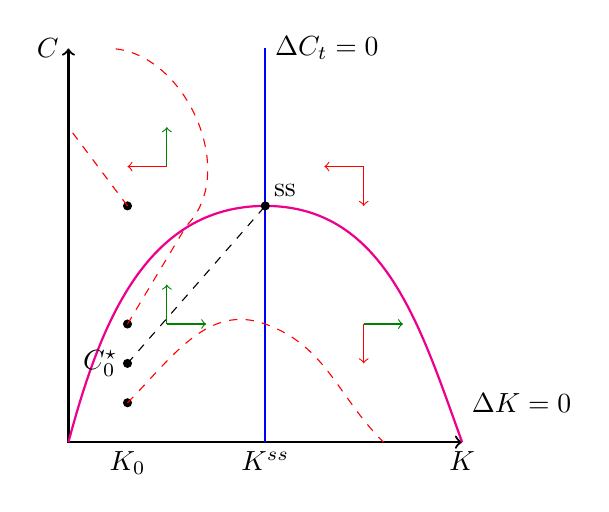
\begin{tikzpicture}[scale=0.5]
			\draw[thick, <->] (0,10)--(0,0)--(10,0);
			\node[below] at (10,0) {$K$};
			\node[left] at (0,10) {$C$};
			\node[below] at (5,0) {$K^{ss}$};
			\draw[thick, blue] (5,0)--(5,10);
			\node[right] at (5,10) {$\Delta C_t = 0$};
			
			\draw[->,Green] (2.5,7)--(2.5,8);
			\draw[->,Green] (2.5,3)--(2.5,4);
			\draw[->,red] (7.5,7)--(7.5,6);
			\draw[->,red] (7.5,3)--(7.5,2);
			
			\draw[thick, magenta] (0,0) to[out = 75, in = 180] (5,6);
			\draw[thick, magenta] (5,6) to[out = 0, in = 110] (10,0);
			
			\node[right] at (10,1) {$\Delta K = 0$};
			
			\draw[->,red] (2.5,7)--(1.5,7);
			\draw[->,Green] (2.5,3)--(3.5,3);
			\draw[->,red] (7.5,7)--(6.5,7);
			\draw[->,Green] (7.5,3)--(8.5,3);
			
			\node[above] at (5.5,6) {ss};
			\draw[fill] (5,6) circle(0.1);
			
			\node[below] at (1.5,0) {$K_0$};
			
			\draw[fill] (1.5,2) circle(0.1);
			\draw[fill] (1.5,3) circle(0.1);
			\draw[fill] (1.5,1) circle(0.1);
			\draw[fill] (1.5,6) circle(0.1);
			
			\node[left] at (1.5,2) {$C_0\opt$};
			
			\draw[dashed] (1.5,2)--(5,6);
			\draw[red,dashed] (1.5,3) to (3,5.5) to[in=0] (1,10);
			\draw[red,dashed] (1.5,1) to[in=160] (5,3) to[out=-20,in=135] (8,0);
			\draw[red,dashed] (1.5,6) to (0,8);
			
		\end{tikzpicture}
		\caption{Phase Diagram for RBC Model}
		\label{fig:rbc_phase}
	\end{figure}
	The steps to generating this are:
	\begin{enumerate}
		\item Find the line where $\Delta C_t = 0$, fix $K^{ss}$ at that level
		\item Suppose that $K_{t+1} = K_t$ ($\Delta K_t = 0$), so $C_t = K_t^\alpha - \delta_k K_t$
		\item Fix $K_0$, and see where the economy would go at any initial $C_0$. There exists a unique $C\opt_0$ such that $(K_0,C\opt_0)$ is \blue{saddle path stable}. It is the unique stable equilibrium.
	\end{enumerate}
\end{definition}

\begin{remark}
	Intuitively, we are thinking about testing every possible $C_0$, and figuring out which paths end up at the steady state (and satisfy the model equations). We can also work this out algorithmically.
\end{remark}

\begin{algorithm}
	\red{(Shooting Method)} Fix some $K_0$. Guess $C_0$, which gives you $K_1$ and $C_1$. Repeat this $T$ times for ``fairly large'' $T$, ending with $K_T,C_T$. We then check if the economy is close to the steady state. Imagine that we are making a function $K^T(K_0,C_0)$, and checking whether
	\[
	K^T(K_0,C_0) - K^{ss} \equiv 0
	\]
	Note well the concept of ``fairly large'' -- we need enough periods to get to the steady state, but not so many that we end with \texttt{Inf} or \texttt{NaN} or something like that. We will use \texttt{fsolve} in Matlab to work through this. This function implements Newton-Raphson to find the optimal guess of $C_0$. It will have issues around $T$, and the usual numerical issues for nonlinear equations, but is fairly consistent.
\end{algorithm}

\begin{remark}
	``This is \href{https://www.angrybirds.com/}{Angry Birds}!'' -- \href{https://www.chahrour.net/}{Ryan Chahrour}, Ph.D.
\end{remark}

We can also implement the opposite method!

\begin{algorithm}
	\red{(Reverse Shooting Method)} We will guess some $(K_T,C_T)$ close to the steady state, and reverse the logical process -- get $(K_{T-1},C_{T-1})$, then $(K_{T-2},C_{T-2})$, all the way to $(K_0,C_0)$. We now have a function $C_0(C_T)$, and solve the equation
	\[
	K_0^\alpha - C_0(C_T) + K_1 - (1-\delta_k)K_0 \Longleftarrow \texttt{fzero}
	\]
	This algorithm is nice because you tend to not have the \texttt{Inf} / \texttt{NaN} issues that the normal shooting method runs into.
\end{algorithm}

However, Ryan has his own preferred approach to shooting.

\begin{algorithm}
	\red{(Chahrour Shooting)} Fix $K_0$, and fix $C_T = C^{ss}$ (an initial and a terminal condition). We will guess an \emph{entire sequence} of $K$'s and $C$'s. We want to guess
	\[
	\matrixp{C_0 & C_1 & C_2 & \cdots & \boxed{C_T} \\\\ \boxed{K_0} & K_1 & K_2 & \cdots & K_t \\ }
	\]
	Where $K_0$ and $C_T$ are fixed. We will check the Euler equation and the resource constraint at every time $t$, and will solve $F(\{C\},\{K\})$ using (something similar to) \texttt{fsolve}. Intuitively, we are pinning down the starting and ending points, and we correct the path at every point -- rather than going through the whole path and seeing how correct it is, we make small changes every step. Since the starting point is precise, we know that it will not go to infinity or zero. It is \emph{very} numerically stable, though it is slow.
\end{algorithm}


\paragraph{Matching Models with Data: a short, somewhat unrelated comment} Imagine that you have a spectrum of how related the model is with the data. This might look something like

\begin{figure}[h]
	\centering
	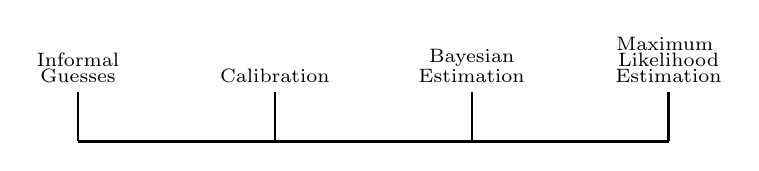
\begin{tikzpicture}[scale=1.25]
		\draw[thick] (0,0)--(6,0);
		
		\node[above] at (0,0.5) {$\substack{\text{Informal} \\ \text{Guesses}}$};
		\node[above] at (2,0.5) {$\substack{\\ \text{Calibration}}$};
		\node[above] at (4,0.5) {$\substack{\text{Bayesian} \\ \text{Estimation}}$};
		\node[above] at (6,0.5) {$\substack{\text{Maximum } \\ \text{Likelihood}\\ \text{Estimation}}$};
		
		\draw[thick] (0,0)--(0,0.5);
		\draw[thick] (2,0)--(2,0.5);
		\draw[thick] (4,0)--(4,0.5);
		\draw[thick] (6,0)--(6,0.5);
	\end{tikzpicture}
\end{figure}

Informal guesses are informal guesses. Calibration has some parameters based on outside evidence, and some chance to match a few moments of the data. Bayesian Estimation is more formal, uses a likelihood function, but naturally incorporates priors. Maximum likelihood estimation has no priors, and is all based on the data.


\subsection{Lagrangian Approach (Decentralized)}

\begin{model}
	\red{(Decentralized Labor Search)} Before this, we've been working on the social planner's problem. Often, we can reference the Welfare Theorems to say that this is equivalent to the decentralized model. We cannot do this here, so we will work through the households, firms, and market clearing conditions to find a solution.
	
	\paragraph{Households} Our households are relatively simple, because they don't make a labor choice. They solve the Lagrangian
	\[
	\max_{\{C_t,\Gamma_t\}} \expect \sum_{t=0}^\infty  \beta^t \curll \frac{C_t^{1-\sigma}}{1-\sigma} + \lambda_t \barl W_tN_t + \Gamma_{t-1} (D_t + P_t) - C_t - \Gamma_t P_t\barr \curlr
	\]
	where $C_t$ is consumption, $\sigma$ is the coefficient of relative risk aversion, $\lambda_t$ is the Lagrange multiplier on the budget constraint, $W_t$ is the wage rate, $N_t$ is the amount of labor supplied by the household, $\Gamma_t$ is the number of shares of the company owned, $D_t$ is the dividend per share, $P_t$ is the price of a share, and $\beta$ is the discount factor. Everything is indexed to time $t$.
	
	The household's first order conditions are
	\begin{align*}
		C_t^{-\sigma} &= \lambda_t &&(C) \\
		\lambda_t P_t &= \beta \expect \barl \lambda_{t+1} (D_{t+1} + P_{t+1})\barr &&(\Gamma)
	\end{align*}
	The second FOC becomes
	\[
	P_t = \beta \expect \barl \underbrace{\parl \frac{C_{t+1}}{C_t}\parr^{-\sigma}}_{\substack{ \text{Stochastic} \\ \text{Discount Factor}}}(D_{t+1} + P_{t+1})\barr
	\]
	Note that $\Gamma_t = 1$ for a representative agent model.
	
	\paragraph{Firms} The firm's problem assumes that they take wages and the probability that a vacancy gets filled as given. They solve the Lagrangian
	\begin{align*}
		\max_{\{Y_t,I_t,V_t,K_{t+1},N_{t+1}\}} \expect \sum_{t=0}^\infty \beta^t &\Bigg\{\frac{\lambda_t}{\lambda_0} \barl Y_t - W_t N_t - I_t - \phi_n V_t\barr \\
		&+ \frac{1}{\lambda_0} \Gamma_{1,t}\barl (1-\delta_n)N_{t-1} + V_tQ_t - N_t\barr  \\
		&+ \frac{1}{\lambda_0} \Gamma_{2,t}[(1-\delta_k)K_t + I_t - K_{t+1}] \\
		&+ \frac{1}{\lambda_0} \Gamma_{3,t} \barl AK_t^\alpha N_t^{1-\alpha} - Y_t \barr \Bigg\}
	\end{align*}
	The firm's first order conditions are
	\begin{align*}
		\lambda_t &= \Gamma_{3,t} &&(Y) \\
		\lambda_t &= \Gamma_{2,t} &&\;(I)\\
		\Gamma_{1,t} &= \lambda_t \frac{\phi_n}{Q_t} &&(V) \\
		\frac{\Gamma_{2,t}}{\lambda_0} &= \beta \expect \barl \frac{\Gamma_{3,t+1}}{\lambda_0} A_{t+1} \alpha \parl \frac{K_{t+1}}{N_{t+1}}\parr^{\alpha - 1} + \frac{1}{\lambda_0} \Gamma_{2,t+1} (1-\delta_k) \barr &&(K) \\
		0 &= -\frac{\lambda_t}{\lambda_0} W_t - \frac{1}{\lambda_0} \Gamma_{1,t} + \frac{1}{\lambda_0} \Gamma_{3,t} A_t \parl \frac{K_t}{N_t}\parr^\alpha (\alpha - 1) + \frac{\beta}{\lambda_0} \expect[\Gamma_{1,t+1}(1-\delta_n)] &&(N)
	\end{align*}
	We can reorganize these first order conditions as
	\begin{align*}
		\underbrace{\frac{\phi_n}{\textcolor{red}{Q_t}}}_{\text{Cost}} &= \underbrace{A_t \parl \frac{K_t}{N_t}\parr^\alpha (1-\alpha) - \textcolor{red}{W_t}}_{\text{Net Benefit, } MPL_t - W_t} + \beta \expect\barl \underbrace{\frac{\lambda_{t+1}}{\lambda_t} (1-\delta_n) \frac{\phi_n}{\textcolor{red}{Q_{t+1}}}}_{\text{Expected Savings Tomorrow}} \barr &&\text{(Decentralized)}
	\end{align*}
	Recall that the Social Planner's Problem gave:
	\begin{align*}
		\frac{\phi_n}{\textcolor{blue}{M_v(\cdot)}} &= A_t \parl \frac{K_t}{N_t}\parr^\alpha (1-\alpha) + \beta \expect\barl \frac{\lambda_{t+1}}{\lambda_t} (1-\delta_n) \frac{\phi_n}{\textcolor{blue}{M_v(\cdot)}}\barr  &&\text{(Social Planner)}
	\end{align*}
	where $M_v(\cdot) = \chi \varepsilon V_t^{\varepsilon - 1}S_t^{1-\varepsilon}$. Consider the differences in these two equations. We have that the probability of a vacancy being matched is defined as
	\[
	Q_t = \frac{\text{Matches}}{\text{Vacancies}} = \frac{\chi V_t^\varepsilon S_t^{1-\varepsilon}}{V_t} = \chi \parl \frac{S_t}{V_t}\parr^{1-\varepsilon}
	\]
	while the marginal increase in the number of jobs created by a marginal posting is
	\[
	M_v(V_t,S_t) = \chi\varepsilon\parl \frac{S_t}{V_t}\parr^{1-\varepsilon}
	\]
	If we plug these into our above Euler equations, we get that
	\begin{align*}
		\frac{\phi_n}{\chi}\parl \frac{V_t}{S_t} \parr^{1-\varepsilon} &= MPL_t \textcolor{red}{ - W_t} + \beta \expect \barl \frac{\lambda_{t+1}}{\lambda_t} (1-\delta_n) \frac{\phi_n}{\chi}\parl \frac{V_{t+1}}{S_{t+1}}\parr^{1-\varepsilon}\barr &&\text{(Decentralized)} \\
		\frac{\phi_n}{\chi\textcolor{blue}{\varepsilon}}\parl \frac{V_t}{S_t} \parr^{1-\varepsilon} &= MPL_t  + \beta \expect \barl \frac{\lambda_{t+1}}{\lambda_t} (1-\delta_n) \frac{\phi_n}{\chi\textcolor{blue}{\varepsilon}}\parl \frac{V_{t+1}}{S_{t+1}}\parr^{1-\varepsilon}\barr &&\text{(Social Planner)} 
	\end{align*}
The first difference is that the social planner can internalize the fact that the probability of a successful matching decreases when an additional vacancy is posted ($\textcolor{red}{\varepsilon}$), but the firm in the decentralized economy cannot do that.

The second difference is that in the decentralized economy, the firm gets lower benefits than the marginal social benefits ($\textcolor{red}{-W_t}$), as they only get to keep the marginal product after paying the wage, while the social planner just experiences the entire marginal product as a benefit.

These two models coincide only if
\[
\varepsilon MPL_t = MPL_t - W_t
\]

\paragraph{Market Clearing} In a market clearing setting, we will necessarily have that for the shares, $\Gamma_t = 1$. Treating $\Gamma_t$ as a choice variable is useful only for pricing the firm's shares. We will also have that the matching function from before holds when the market clears -- reprinting it, we have that
\[
Q_t = \frac{\text{Matches}}{\text{Vacancies}} = \frac{\chi V_t^\varepsilon S_t^{1-\varepsilon}}{V_t} = \chi \parl \frac{S_t}{V_t}\parr^{1-\varepsilon}
\]
We also technically have that output clears, meaning that $Y_t = C_t + I_t + \phi_n V_t$. The first and third of these conditions are largely trivial, the real relevant one is $Q_t$.
\end{model}

\paragraph{Nash Bargaining of Wages} Above, we identified that the decentralized economy coincides with the social planner's problem only if $\varepsilon MPL_t = MPL_t - W_t$. Let's think more about when this might happen. In general, in search models there is a surplus for a match, for both the worker and the firm. Let's assume that the worker gets zero earnings for not having a job. Any wage between 0 and $MPL_t \;(+ \text{ continuation})$ would be consistent with equilibrium. We have that the continuum of possible wages is

\begin{figure}[h]
	\centering
	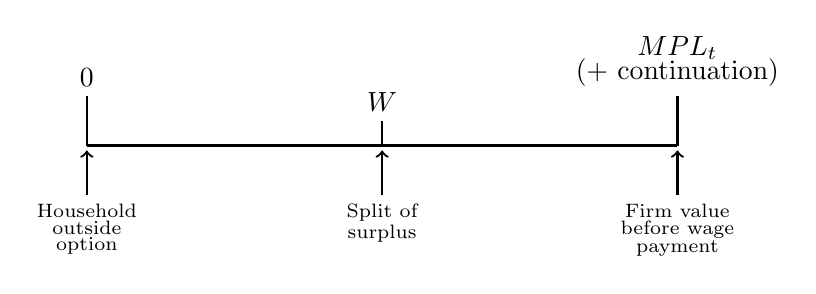
\begin{tikzpicture}[scale=1.25]
		\draw[thick] (0,0)--(6,0);
		
		\node[above] at (0,0.5) {0};
		\node[above] at (6,0.77) {$MPL_t$};
		\node[above] at (6,0.5) {$(+ \text{ continuation})$};
		
		\draw[thick] (0,0)--(0,0.5);
		\draw[thick] (6,0)--(6,0.5);
		
		\node[below] at (0,-0.5) {$\substack{ \text{Household} \\\text{outside} \\ \text{option}}$};
		\draw[->,thick] (0,-0.5)--(0,-0.05);
		\draw[->,thick] (6,-0.5)--(6,-0.05);
		\node[below] at (6,-0.5) {$\substack{ \text{Firm value} \\\text{before wage} \\ \text{payment}}$};
		
		\draw[thick] (3,0)--(3,0.25);
		\node[above] at (3,0.25) {$W$};
		\draw[->,thick] (3,-0.5)--(3,-0.05);
		\node[below] at (3,-0.5) {$\substack{\text{Split of} \\ \text{surplus}}$};
	\end{tikzpicture}
\end{figure}

We will think of a particular wage paradigm, known as \blue{Nash bargaining}, in which workers and firms bargain over the current wage, taking as given the wage that will be realized in future periods. 

First, we need to calculate the surplus that the firms and the workers receive for a given equilibrium wage. Denote $\bar{W}_t(w_t)$ to be the workers' surplus and $J_t(w_t)$ to be the firms' surplus. Given relative bargaining power $\eta$ and $(1-\eta)$ for both sides, the Nash bargaining solution maximizes:
\[
\max_{w_t} [\bar{W}_t(w_t)]^\eta [J_t(w_t)]^{1-\eta}
\]
which captures the idea that firms and workers share the surplus of a match according to their bargaining powers. 

Let's find closed forms for the worker and firm surplus. For the firm, their outside option is zero, because they will pay no wage and earn no profit. If they do make an agreement, their value is
\[
J_t(w_t) = \underbrace{MPL_t - w_t}_{\text{Today's profits}} + \underbrace{\beta (1-\delta_n) \expect \barl \parl \frac{C_{t+1}}{C_t}\parr^{-\sigma} J_{t+1} \barr}_{\text{Future value if not separated}}
\]

Note that the worker's benefits of not being matched should be zero -- we think that they get no wage and no dividends. We are assuming that $S_t = 1$, so the additional unemployed worker does not affect the stock tomorrow. Their benefits if they do get matched are
\[
\bar{W}_t(w_t) = \underbrace{w_t}_{\text{Today's wage}} + \underbrace{\beta (1-\delta_n)\expect \barl \parl \frac{C_{t+1}}{C_t}\parr^{-\sigma} \bar{W}_{t+1} \barr}_{\text{Future value if not separated}} + \underbrace{\beta \delta_n \expect\barl \parl \frac{C_{t+1}}{C_t}\parr^{-\sigma} \bar{U}_{t+1} \barr}_{\text{Unemployment benefits; } = 0}
\]
Taking first order conditions of the problem with respect to $w_t$, we get that
\[
\eta \bar{W}_t(w_t)^{\eta - 1} J_t(w_t)^{1 - \eta} +  \bar{W}_t(w_t)^{\eta} (1-\eta)J_t(w_t)^{-\eta} = 0
\]
which rearranges to
\[
\bar{W}_t(w_t) = \frac{\eta}{1-\eta} J_t(w_t)
\]
Substituting the analytic forms for $\bar{W}$ and $J$, and using this equation again, we get that
\[
\frac{\eta}{1-\eta} \curll MPL_t - w_t + \beta (1-\delta_n) \expect\barl \parl \frac{C_{t+1}}{C_t}\parr^{-\sigma} J_{t+1}(w_t)\barr \curlr = w_t + \beta (1-\delta_n) \expect \barl \parl \frac{C_{t+1}}{C_t}\parr^{-\sigma} \underbrace{\frac{\eta}{1-\eta} J_{t+1}(w_t)}_{\bar{W}_{t+1}(w_t)}\barr
\]
Simplifying, we get that
\[
\eta (MPL_t - w_t) = (1-\eta)w_t \Longrightarrow \boxed{w_t\opt = W_t = \eta \cdot MPL_t + (1-\eta) \cdot 0}
\]
which is the solution to the Nash bargaining problem. The decentralized problem and the social planner's problem coincide only if $\eta = 1-\varepsilon$, which we call the \blue{Hosios Condition} (after \href{https://academic.oup.com/restud/article-abstract/57/2/279/1551634}{Hosios (1990)}).

\paragraph{Intuition.} Remember that this is not a First Welfare Theorem (Theorem~\ref{thm:first_welfare}) economy. The fact that there can be efficiency here is actually somewhat strange -- we would not expect that. However, we can think about this as a sort of balancing act between the private benefit of hiring a worker and the social benefit of hiring a worker. We can think about the following conditions:

\begin{align*}
	\text{Private Benefit} &= MPL_t - W_t \qquad\qquad <  &&\text{Social Benefit} = MPL_t \\
	\text{Private Cost} &= \frac{\phi_n}{\chi}\parl \frac{V_t}{S_t}\parr^{1-\varepsilon} \qquad\quad\;\;\; <  &&\text{Social Cost}\;\;\;\; = \frac{\phi_n}{\chi\varepsilon} \parl \frac{V_t}{S_t}\parr^{1-\varepsilon}
\end{align*}

The first inequality would indicate that firms tend to under-hire, and the second would indicate that firms tend to over-hire. The Hosios Condition is the exact point where they exactly cancel out, and the firm hires at exactly at the social optimum. When $\eta > 1-\varepsilon$, firms under-hire (because worker bargaining power is too high), and when $\eta < 1-\varepsilon$, firms over-hire (because firm bargaining power is too high).


\subsection{Value Function Approach (Social Planner)}

\paragraph{Roadmap.} We have seen the same problem through the social planner's perspective and the decentralized perspective, using the same strategy -- solving the Lagrangian. We will now move to the same problem(s), solved through value function iteration. We've also seen two main techniques -- log-linearization, which is linear but allows for uncertainty, and the shooting method, which is nonlinear but assumes perfect foresight. Both of these techniques can solve both the planner's problem and the decentralized problem, but say nothing about the value function.

Value function iteration is both nonlinear and allows for uncertainty, but can only solve the planner's problem -- it works through the value function, which cannot be used in a decentralized way. 

After value function iteration, we will explore projection methods, which are nonlinear, allow for uncertainty, and work for both the planner's problem and the decentralized problem; at the cost of time of implementation. We will explore that through the Lagrangian approach.

\begin{model}
	\red{Value Function (Social Planner)} The social planner has the Bellman Equation:
	\[
	V(K_t,N_{t-1},A_t) = \max_{K_{t+1},N_t} U_t(C_t) + \beta \expect \barl V(K_{t+1},N_t,A_{t+1}) \barr
	\]
	subject to
	\begin{align*}
		C_t &= Y_t - I_t - \phi_n V_t \\
		&= A_tK_t^\alpha N_t^{1-\alpha} - (K_{t+1} - (1-\delta_k)K_t) - \phi_n \parl \frac{N_t - (1-\delta_n)N_{t-1}}{\chi}\parr^\frac{1}{\varepsilon}
	\end{align*}
	where the second equality uses the fact that $Y_t = A_tK_t^\alpha N_t^{1-\alpha}$, $I_t = K_{t+1} - (1-\delta_k)K_t$, and rearranging $N_t = (1-\delta_n)N_{t-1} + \chi V_t^\varepsilon S_t^{1-\varepsilon}$, we get that
	\[
	V_t = \parl \frac{N_t - (1-\delta_n)N_{t-1}}{\chi}\parr^\frac{1}{\varepsilon}
	\]
	Substituting into the planner's Bellman equation, it becomes
	\begin{align*}
		V(K_t,N_{t-1},A_t) = \max_{K_{t+1},N_t} &U_t\parl A_tK_t^\alpha N_t^{1-\alpha} - (K_{t+1} - (1-\delta_k)K_t) - \phi_n \parl \frac{N_t - (1-\delta_n)N_{t-1}}{\chi}\parr^\frac{1}{\varepsilon}\parr \\
		&+ \beta \expect \barl V(K_{t+1},N_t,A_{t+1}) \barr
	\end{align*}
	The first order conditions are:
	\begin{align*}
		(K_{t+1})\qquad 0 &= -U'(C_t) + \beta \expect[V_K(K_{t+1},N_t,A_{t+1}) ] \\
		(N_t) \qquad 0 &= U'(C_t)\barl - \frac{\phi_n}{\chi \varepsilon}\parl \frac{N_t - (1-\delta_n)N_{t-1}}{\chi}\parr^{\frac{1-\varepsilon}{\varepsilon}} + A_t \parl \frac{K_t}{N_t}\parr^\alpha (1-\alpha) \barr + \beta \expect[V_N(K_{t+1},N_t,A_{t+1}) ]
	\end{align*}
\end{model}

\paragraph{Envelope Theorem Aside.}

We need to take the derivatives of $V_K(\cdot)$ and $V_N(\cdot)$. The Envelope Theorem tells us that we can ignore the chain rule in taking these, and proceed with just the obvious terms. We will do a quick proof for $V_K(\cdot)$.

Suppose that we know the policy functions already, and call them $K_{t+1} = \textbf{K}(K_t,N_{t-1},A_t)$ and $N_t = \textbf{N}(K_t,N_{t-1},A_t)$. Our value function is now:
\begin{align*}
	V(K_t,N_{t-1},A_t) = &U\parl A_tK_t^\alpha \textbf{N}(\cdot)^{1-\alpha} - (\textbf{K}(\cdot) - (1-\delta_k)K_t) - \phi_n \parl \frac{\textbf{N}(\cdot) - (1-\delta_n)N_{t-1}}{\chi}\parr^\frac{1}{\varepsilon}\parr \\
	&+ \beta \expect[V(\textbf{K}(\cdot),\textbf{N}(\cdot),A_{t+1})]
\end{align*}
Note that we don't have the max operator anymore! We can take the derivative with respect to $K_t$, using all of the appropriate chain rules. We get that
\begin{align*}
	V_K(K_t,N_{t-1},A_t) &= U'(C_t) \cdot \barl A_t \parl \frac{K_t}{N_t}\parr^{\alpha - 1}\alpha + (1-\delta_k)\barr \\
	&- U'(C_t) \cdot \frac{\partial \textbf{K}}{\partial K_t} + \beta \expect \barl V_K(K_{t+1},N_t,A_{t+1}) \barr\frac{\partial \textbf{K}}{\partial K_t} \\
	&+ U'(C_t) \barl \frac{\phi_n}{\varepsilon\chi} \parl\frac{N_t - (1-\delta_n)N_{t-1}}{\chi} \parr^{\frac{1-\varepsilon}{\varepsilon}} + A_t \parl \frac{K_t}{N_t}\parr^\alpha (\alpha - 1)\barr \frac{\partial \textbf{N}}{\partial K_t} \\
	&+ \beta \expect\barl V_N(K_{t+1},N_t,A_{t+1})\barr \frac{\partial \textbf{N}}{\partial K_t}
\end{align*}
However, from our first order conditions above, if we are at an optimum, we have that the second line should evaluate to zero! Also, the third and fourth lines should evaluate to zero! We finally have that
\[
V_K(K_t,N_{t-1},A_t) = U'(C_t) \cdot \barl A_t \parl \frac{K_t}{N_t}\parr^{\alpha - 1}\alpha + (1-\delta_k)\barr
\]

\paragraph{Back to FOCs.} Using the Envelope Theorem, we have that
\begin{align*}
	V_K(K_t,N_{t-1},A_t) &=  U'(C_t) \cdot \barl A_t \parl \frac{K_t}{N_t}\parr^{\alpha - 1}\alpha + (1-\delta_k)\barr \\
	V_N(K_t,N_{t-1},A_t) &= U'(C_t) \cdot \barl \frac{\phi_n}{\varepsilon\chi} \parl \frac{N_t - (1-\delta_n)N_{t-1}}{\chi}\parr^\frac{1-\varepsilon}{\varepsilon}(1-\delta_n)\barr
\end{align*}

Combining the first order conditions and the Envelope Theorem results, we get that
\begin{align*}
	U_t'(\cdot) &= \beta \expect \barl U'_{t+1}(\cdot) \parl A_{t+1} \parl \frac{K_{t+1}}{N_{t+1}}\parr^{\alpha - 1} \alpha + (1-\delta_k) \parr \barr \\
	U_t'(\cdot) \barl \frac{\phi_n}{\varepsilon\chi} \parl \frac{N_t - (1-\delta_n)N_{t-1}}{\chi}\parr^\frac{1-\varepsilon}{\varepsilon} \barr &= U'_t(\cdot)\barl A_t \parl \frac{K_t}{N_t}\parr^{\alpha}(1-\alpha) \barr \\
	&\qquad \qquad+ \beta \expect\barl U'_{t+1}(\cdot) \parl \frac{\phi_n}{\varepsilon\chi} \parl \frac{N_{t+1} - (1-\delta_n)N_{t}}{\chi}\parr^\frac{1-\varepsilon}{\varepsilon}(1-\delta_n)\parr \barr
\end{align*}
Rearranging and imposing the functional form for the matching function, these clearly become the capital and labor Euler equations we found above in the planner's problem.



\subsection{Mathieu Interlude (Labor Search Formalities)}

\paragraph{Motivation.} We spent a lot of time last quarter on the neoclassical growth model. It has some distinct drawbacks: it assumes a unique labor market with a market clearing wage; it does not capture the process of finding a job particularly well (think search, vacancy posting, matching, bargaining, etc.); and there is no unemployment! We turn to a new class of models that take these details seriously, for which Peter Diamond, Christopher Pissarides, and Dale Mortensen won the \href{https://www.nobelprize.org/prizes/economic-sciences/2010/summary/}{2010 Nobel Prize}. 

For this section, we reference \href{https://mitpress.mit.edu/9780262038669/recursive-macroeconomic-theory/}{Ljundqvist and Sargent} chapters 6 and 26, as well as \href{https://www.aeaweb.org/articles?id=10.1257/002205105775362014}{Roger, Shimer, \& Wright (2005)} and \href{https://mitpress.mit.edu/9780262533980/equilibrium-unemployment-theory/}{Pissarides (2000)}.

\paragraph{Math preliminaries} Let $p$ be a random variable with CDF $F(P) = \prob\{p \le P\}$. Assume that $F(0) = 0$, $F(\infty) = 1$, and $F$ continuous from the right. Assume that $p$ is bounded above with probability 1 -- so $\exists B \st F(B) = 1$. Recall that the mean of $p$ is given by
\[
\expect[p] = \int_0^B pdF(p)
\]
Letting $u = 1- F(p)$ and $v = p$, we can integrate by parts and get that
\[
\expect[p] = \int_0^B pdF(p) = \int_0^B (1-F(p)) dp = B - \int_0^B F(p)dp
\]

Now consider two independent random variables $p_1,p_2 \sim F$ and consider the event $\{(p_1 \le p) \cap (p_2 \le p)\}$. This event happens with probability $(F(p))^2$, and this is equivalent to the event $\{\max\{p_1,p_2\} \le p\}$. Using our previous result, we have that
\[
\expect[\max\{p_1,p_2\}] = B - \int_0^B F(p)^2 dp
\]
Generalizing with $n$ independent draws, we get that
\[
M_n \equiv \expect[\max\{p_1,p_2,\dots,p_n\}] = B - \int_0^B F(p)^n dp
\]


\paragraph{Stigler Model}

\begin{model}
	\red{Stigler Search Model} (from \href{https://home.uchicago.edu/~vlima/courses/econ200/spring01/stigler.pdf}{Stigler (1961)}) This is a partial equilibrium model of an agent looking for a job. We have a risk-neutral agent who samples i.i.d. wages from some distribution $F(w)$ with the earlier assumptions. Their \emph{ex ante} decision of how many wages to gather is $n$, and getting a wage offer has cost $c$. How many offers should they ask for? 
	
	\begin{definition}
		The \blue{expected gain} from an additional draw is
		\begin{align*}
			G_n &= M_n - M_{n-1} = B - \int_0^B F(p)^n dp - \parl B - \int_0^B F(p)^{n-1}dp\parr \\
			&= \int_0^B F(p)^{n-1}dp - \int_0^B F(p)F(p)^{n-1}dp \\
			&= \int_0^B F(p)^{n-1}(1-F(p))dp
		\end{align*}
		Note that $G_n$ decreases with $n$, and $\lim_{n\to\infty}G_n = 0$. The optimal rule is to pick $n$ such that $G_n \ge c > G_{n+1}$. 
	\end{definition}
\end{model}
\begin{question}
		What's weird with this model? Static search. We tend to think of searching for a job as a sequential thing, not a single time drawing a large number of wages. \href{https://academic.oup.com/qje/article-abstract/84/1/113/1931495}{McCall (1970)} fixes this.
\end{question}

Consider a class of distributions $F(p,r) = \prob\{P_r \le p)$ indexed by $r \in \reals$. $F(p,r)$ is differentiable with regard to $r$ for all $p \in [0,B]$, and there exists $B \in \reals$ such that $F(B,r) = 1$, and $F(0,r) = 0 \forall r \in \reals$. Since $\expect[p] = B - \int_0^B F(p,r)dp$, two distributions with the same $\int_0^B F(p,r)dp$ have the same mean.

\begin{definition}
	We say that a distribution $r_2$ is a \blue{mean-preserving spread} of a distribution $r_1$ if
	\begin{enumerate}
		\item Identical means condition:
		\[
		\int_0^B (F(\theta,r_1) - F(\theta,r_2))d\theta = 0
		\]
		\item Single-crossing property: There exists $\hat{\theta} \in (0,B)$ such that
		\[
		F(\theta,r_2) - F(\theta,r_1) \le 0 \;(\ge 0) \text{ when } \theta \le \;(\ge)\; \hat{\theta}
		\]
		
	\end{enumerate}
	This is illustrated in Figure 2.
	\begin{figure}[h]
	\centering
	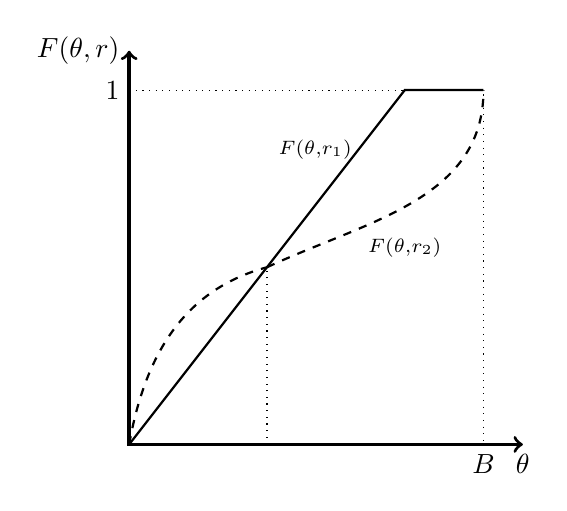
\begin{tikzpicture}[scale = 0.5]
		\draw[very thick, <->] (0,10)--(0,0)--(10,0);
		
		\node[left] at (0,10) {$F(\theta,r)$};
		\node[below] at (10,0) {$\theta$};
		\node [below] at (9,0) {$B$};
		\node[left] at (0,9) {$1$};
		\draw[dotted] (0,9)--(9,9)--(9,0);
		\draw[thick] (0,0)--(7,9)--(9,9);
		\draw[thick,dashed] (0,0) to[out=80,in=195] (3.5,4.5);
		\draw[thick,dashed] (3.5,4.5) to[out=25,in=-90] (9,9);
		
		\draw[dotted] (3.5,0)--(3.5,4.5);
		\node[left] at (5.9,7.5) {${\scriptstyle F(\theta,r_1)}$};
		\node[below] at (7,5.5) {${\scriptstyle F(\theta,r_2)}$};
	\end{tikzpicture}
	\caption{Mean-Preserving Spreads}
	
\end{figure}

	Properties 1 and 2 imply that 
	\[
	\int_0^y (F(\theta,r_2) - F(\theta,r_1))d\theta \ge 0 \forall y \in [0,B]
	\]
	For infinitesimal changes in $r$, an increase in $r$ is said to represent a \blue{mean-preserving increase in risk} if
		\[
		\int_0^B F_r(\theta,r) d\theta = 0 \qquad \text{ and } \qquad \int_0^y F_r(\theta,r) d\theta \ge 0 \forall \theta \in [0,B]
		\]
		where $F_r(\theta,r) = \frac{\partial F(\theta,r)}{\partial r}$.
\end{definition}




\begin{model}
	\red{McCall Labor Search} (from \href{https://academic.oup.com/qje/article-abstract/84/1/113/1931495}{McCall (1970)}) An agent searches for a job, taking market conditions as given. Each period the agent draws one offer $w \sim F(W)$, where $F(0) = 0$ and $F(B) = 1$ for some $B < \infty$. The agent can accept or reject the offer. If she rejects, she gets $c$ today and draws another offer tomorrow. If she accepts, she receives $w$ per period forever. 
	
	The agent maximizes
	\[
	\expect\barl \sum_{t=0}^\infty \beta^t y_t\barr
	\]
	where $y_t = c$ if she is unemployed and $y_t = w$ if she is employed at wage $w$. 
\end{model}
\paragraph{Solving the model.} Denote by $v(w)$ the expected value of an offer $w$ for an agent who is deciding whether or not to accept the offer or reject it. If she behaves optimally, we have 
\[
v(w) = \max \curll \frac{w}{1-\beta} , c + \beta \int v(w') dF(w')\curlr
\]
The solution of this Bellman equation is of the form
\[
v(w) = \begin{cases} \frac{\bar{w}}{1-\beta} = c + \beta \int v(w')dF(w')  & \text{ if } w \le \bar{w} \\ \frac{w}{1-\beta} & \text{ if }w > \bar{w} \end{cases}
\]
where $\bar{w}$ is called the \blue{reservation wage}. The agent's value function is illustrated in Figure 3.

\begin{figure}[H]\label{fig:value_mccall}
	\centering
	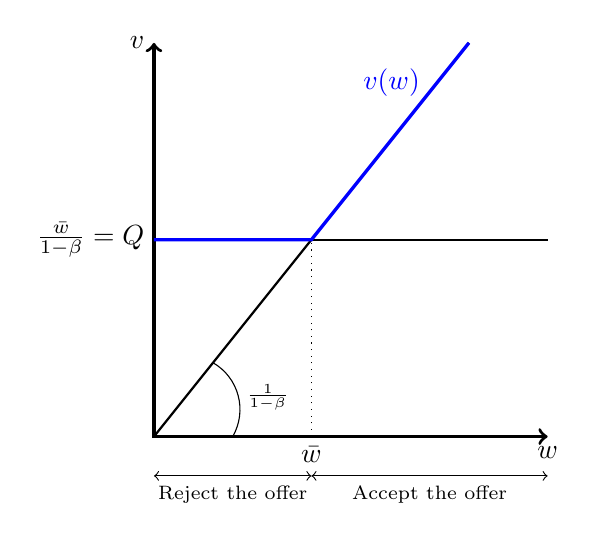
\begin{tikzpicture}[scale = 0.5]
		\draw[very thick, <->] (0,10)--(0,0)--(10,0);
		\node[left] at (0,10) {$v$};
		\node[left] at (0,5) {$\frac{\bar{w}}{1-\beta} = Q$};
		\node[below] at (4,0) {$\bar{w}$};
		\node[below] at (10,0) {$w$};
		
		\draw[black, thick] (0,5)--(10,5);
		\draw[black,thick](0,0)--(8,10);
		\draw[dotted] (4,0)--(4,5);
		\draw (2,0) to[out=60,in=-30] (1.5,15/8);
		\node[right] at (2.1,1) {${\scriptstyle \frac{1}{1-\beta}}$};
		\draw[blue, very thick] (0,5)--(4,5)--(8,10);
		\node[left] at (7,9) {\textcolor{blue}{$v(w)$}};
		
		\draw[<->] (0,-1)--(4,-1);
		\draw[<->] (4,-1)--(10,-1);
		
		\node[below] at (2,-1) {{\scriptsize Reject the offer}};
		\node[below] at (7,-1) {{\scriptsize Accept the offer}};
	\end{tikzpicture}
	\caption{Value per Wage Offer}
	
\end{figure}

 How do we find $\bar{w}$? At $w = \bar{w}$, the agent is indifferent, so
 \[
 \frac{\bar{w}}{1-\beta} = c + \beta \int_0^{\bar{w}} \frac{\bar{w}}{1-\beta}dF(w') + \beta \int_{\bar{w}}^B \frac{w'}{1-\beta}dF(w')
 \]
or
\[
 \frac{\bar{w}}{1-\beta} \int_0^{\bar{w}} dF(w') +  \frac{\bar{w}}{1-\beta}\int_{\bar{w}}^B dF(w') = c + \beta \int_0^{\bar{w}} \frac{\bar{w}}{1-\beta}dF(w') + \beta \int_{\bar{w}}^B \frac{w'}{1-\beta}dF(w')
\]
or
\[
\bar{w} \int_0^{\bar{w}} dF(w') - c = \frac{1}{1-\beta} \int_{\bar{w}}^B (\beta w' - \bar{w}) dF(w')
\]
Adding $\bar{w} \int_{\bar{w}}^B dF(w')$ to both sides, we get
\begin{align*}
\bar{w} - c &= \frac{\beta}{1-\beta} \int_{\bar{w}}^B (w' - \bar{w}) dF(w') \\
&= \beta \expect \barl \frac{w' - \bar{w}}{1-\beta} \midbar w' \ge \bar{w}\barr \prob\curll w' \ge \bar{w}\curlr
\end{align*}
where the left hand side is the cost of searching one more time with offer $\bar{w}$ in hand, and the right hand side is the surplus from searching one more time and getting a better offer. These two things must be equal if the agent is optimizing: $MR = MC$.

We can define the function
\[
h(w) \coloneqq \frac{\beta}{1-\beta} \int_{w}^B (w' - w) dF(w')
\]
Note that: 
\begin{align*}
	h(0) &= \expect\barl \frac{\beta w}{1-\beta} \barr \\
	h(B) &= 0 \\
	h(w) &\text{ is differentiable} \\
	h'(w) &= -\frac{\beta}{1-\beta} (1- F(w)) < 0 \\
	h''(w) &= \frac{\beta}{1-\beta} F'(w) > 0
\end{align*}
$h(w)$ is illustrated in Figure 4.

\begin{figure}[h]
	\centering
	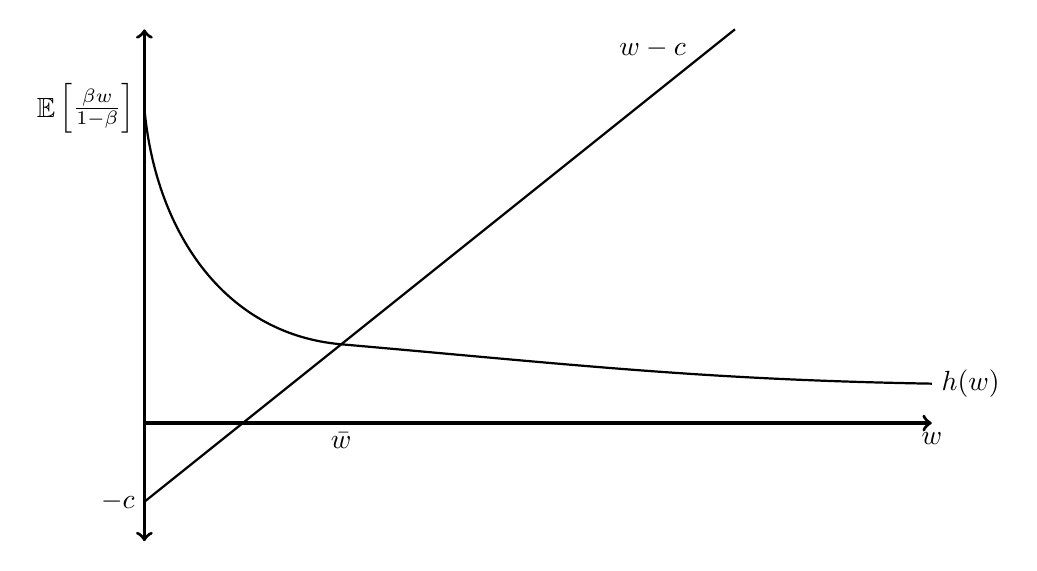
\begin{tikzpicture}[scale = 0.5]
		\draw[very thick, <->] (0,10)--(0,0)--(20,0);
		\draw[very thick, ->] (0,0)--(0,-3);
		\node[left] at (0,8) {$\expect\barl \frac{\beta w}{1-\beta}\barr$};
		\node[left] at (0,-2){$-c$};
		\node[below] at (5,0) {$\bar{w}$};
		\node[below] at (20,0) {$w$};
		\node[right] at (20,1) {$h(w)$};
		\node[left] at (14,9.5) {$w - c$};
		
		
		\draw[thick] (0,-2)--(15,10);
		\draw[thick] (0,8) to[out=-85,in=175] (5,2) to[out=-5,in=179] (20,1);
	\end{tikzpicture}
	\caption{Finding the Reservation Wage, part 1}
\end{figure}

\begin{question}
	What happens when the environment changes? Let's manipulate the equations a bit more.
\end{question}
\begin{align*}
	\bar{w} - c &= \frac{\beta}{1-\beta} \int_{\bar{w}}^B(w' - \bar{w})dF(w') + \frac{\beta}{1-\beta} \int_0^{\bar{w}}(w' - \bar{w}) dF(w') - \frac{\beta}{1-\beta} \int_0^{\bar{w}}(w' - \bar{w}) dF(w') \\
	&= \frac{\beta}{1-\beta} \expect[w]- \frac{\beta}{1-\beta} \bar{w} - \frac{\beta}{1-\beta} \int_0^{\bar{w}}(w' - \bar{w}) dF(w')
\end{align*}
or
\[
\bar{w} - (1-\beta)c = \beta \expect[w] - \beta \int_0^{\bar{w}}(w' - \bar{w}) dF(w')
\]
Integrating by parts, we get
\[
\bar{w} - c = \beta (\expect[w] - c) + \beta \int_0^{\bar{w}}F(w')dw' \equiv \beta(\expect[w] - c) + \beta g(\bar{w})
\]
This relationship is illustrated in Figure 5.

\begin{figure}[H]
	\centering
	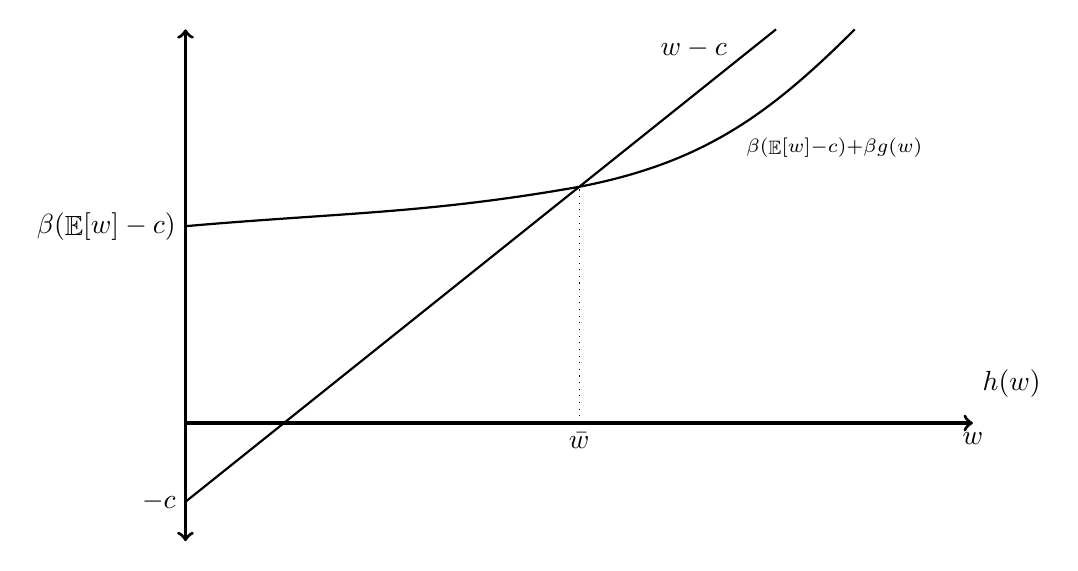
\begin{tikzpicture}[scale = 0.5]
		\draw[very thick, <->] (0,10)--(0,0)--(20,0);
		\draw[very thick, ->] (0,0)--(0,-3);
		\node[left] at (0,5) {$\beta (\expect[w] - c)$};
		\node[left] at (0,-2){$-c$};
		\node[below] at (10,0) {$\bar{w}$};
		\node[below] at (20,0) {$w$};
		\node[right] at (20,1) {$h(w)$};
		\node[left] at (14,9.5) {$w - c$};
		
		\draw[thick] (0,-2)--(15,10);
		\draw[thick] (0,5) to[out=5,in=190] (10,6) to[out=11,in=225] (17,10);
		\draw[dotted] (10,0)--(10,6);
		\node[right] at (14,7) {${\scriptstyle \beta (\expect[w]-c) + \beta g(w)}$};
	\end{tikzpicture}
	\caption{Finding the Reservation Wage, part 2}
\end{figure}

\begin{question}
	What happens when $c$ increases? Both curves move to the right, the reservation wage increases.
\end{question}

\begin{question}
	What happens when there is a mean-preserving increase in risk? $g(\bar{w})$ increases, meaning that the reservation wage increases. Intuition: there are more bad jobs, but we don't care about those. Instead, the agent sees the upside of the better jobs that are available.
\end{question}

\paragraph{Problems with the model.} Firm behavior isn't considered, but it gets weird. Workers follow a reservation wage strategy, so firms do not gain anything for posting $w > \bar{w}$. Firms also do not hire anyone when they post $w < \bar{w}$. Therefore, $F(w)$ will have a unit mass at $\bar{w}$ (\href{https://www.sciencedirect.com/science/article/pii/0022053174900660?via\%3Dihub}{Rothschild (1974)}). Moreover, from \href{https://www.sciencedirect.com/science/article/pii/0022053171900135}{Diamond (1971)},
\begin{align*}
	\bar{w}-c &= \beta(\expect[w] - c) + \beta \int_0^{\bar{w}} F(w')dw' \\
	\bar{w}-c &= \beta(\bar{w} - c) \\
	\bar{w} &= c
\end{align*}
Intuition? Firms know that they can post at $\bar{w}$ and get that everyone will accept. Then workers will re-optimize, and $\bar{w}$ will decrease, and the process will repeat. We will unravel, until $\bar{w} = c$, the theoretical minimum.



\subsection{Value Function Iteration}

Numerically, we are going to be finding a value function (and associated policy functions) that satisfy 
\[
V(K_t,N_{t-1},A_t) = \max_{K_{t+1},N_t} U_t(C_t) + \beta \expect \barl V(K_{t+1},N_t,A_{t+1}) \barr
\]
We need to make some choices:
\begin{enumerate}
\item How should we summarize the state space? Traditionally, we use a discrete grid. We will use an even grid for $K_t$ and $N_{t-1}$, and will use either the Tauchen process (from Mathieu's section) or the Rouwenhorst Method (in the sample code, and see \href{https://karenkopecky.net/Rouwenhorst_WP.pdf}{Kopecky and Suen (2009)} for more).

\item How should we compute expectations? Using the Rouwenhorst approximation weights, essentially.

\item How do we solve for the maximum? We simply optimize over the discrete grid.
\end{enumerate}


\subsection{Projection Methods}

We will begin talking about projection methods, a functional approximation of the problem. Projection methods, as talked about above, are slow but very precise, and deal with nonlinearities nicely. 

The theoretical object we are concerned with is $h(x)$, the continuous policy function. We will approximate it as 
\[
\hat{h}(x) = \sum_{n=1}^N \underbrace{a_n}_{\text{Weights}} \underbrace{b_n(x)}_{\text{Basis functions}}
\]
These basis functions will end up being simple functions in the mathematical sense as well, which is lovely! Mainly, we care about them being numerically simple. We will ideally solve the problem
\[
\min_{\{a_n\}} \int_\mathcal{X} (h(x) - \hat{h}(x))^2 dx
\]
Practically, we will minimize
\[
\min_{\{a_n\}} \sum_{i\in \mathcal{X}} w_i(h(x_i) - \hat{h}(x_i))^2
\]

\paragraph{Special Case.} When $|\mathcal{X}| = N$, we will often be able to find an exact solution, where the minimization problem goes to zero. This is called \blue{interpolation}.

We will make two key choices: the basis functions and the loss function (or interpolation points). We are assuming least squares above, but this would also include the weights $w_i$. 

\paragraph{Choosing Basis Functions.} We have three common choices for basis function:
\begin{enumerate}
	\item \href{https://en.wikipedia.org/wiki/Taylor_series}{Taylor Polynomial}. In the scalar case, we have:
	\[
	a_0 + a_1x + a_2x^2 + \cdots + a_N x^N
	\]
	Positives: this is differentiable. Negative: slow-spanning.
	\item \href{https://en.wikipedia.org/wiki/Chebyshev_polynomials}{Chebyshev Polynomials}. These are polynomials which are composed of trigonometric transformations. There's not a nice closed form for arbitrary $h$, but they have some nice properties generally.

	
	Positives: also differentiable, and quick-spanning. Negative: weird behavior off-grid.
	\item \href{https://www.geophysik.uni-muenchen.de/~igel/Lectures/NMG/08_finite_elements_basisfunctions.pdf}{Finite element basis functions}. These only have local support, and are represented with linear `hat' functions. They are functions which are linear, and a maximum of two of them are non-zero at any one time. We can imagine that we know $h(x)$ at $x = \{0,1,2,\dots,6\}$, and we define $h$ as a weighted average of the relevant basis functions $\omega_i$ with weights $b_i$:
	\[
	\min_{\{b_i\}} \sum_{x_j} \parl h(x_j) - \sum_{i=0}^6 a_i \omega_i(x_j)\parr^2
	\]
	where $\sum_{i=0}^6 a_i \omega_i(x_j) = \hat{h}(x_j)$. It's easiest to think of these graphically.
	\begin{figure}[H]
		\centering
		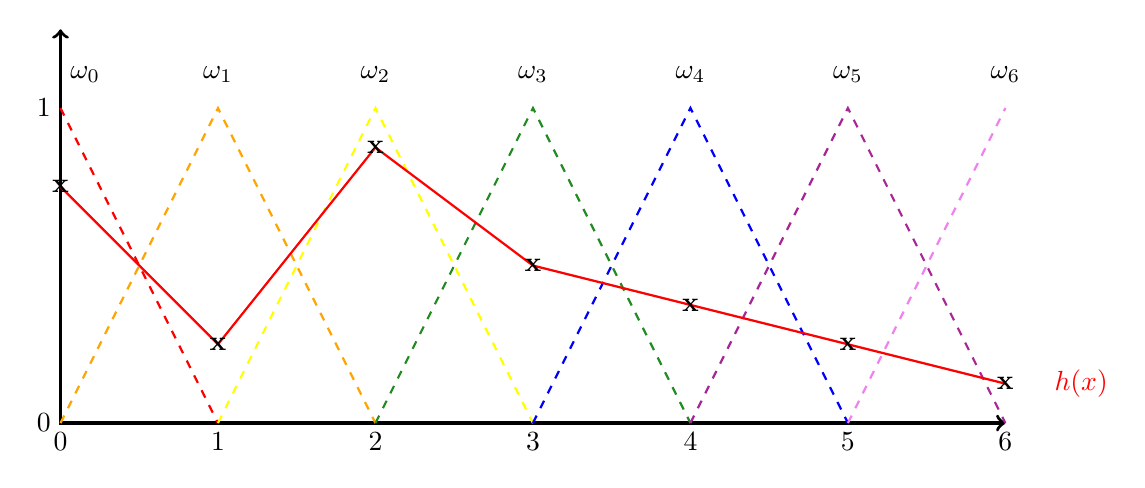
\begin{tikzpicture}
			\draw[very thick, <->] (0,5)--(0,0)--(12,0);
			\node[left] at (0,0) {0};
			\node[below] at (0,0) {0};
			\node[left] at (0,4) {1};
			\node[below] at (2,0) {1};
			\node[below] at (4,0) {2};
			\node[below] at (6,0) {3};
			\node[below] at (8,0) {4};
			\node[below] at (10,0) {5};
			\node[below] at (12,0) {6};
			
			\draw[Orange,dashed,thick] (0,0)--(2,4)--(4,0);
			\draw[Red,dashed,thick] (0,4)--(2,0);
			\draw[Yellow,dashed,thick] (2,0)--(4,4)--(6,0);
			\draw[ForestGreen,dashed,thick] (4,0)--(6,4)--(8,0);
			\draw[Blue,dashed,thick] (6,0)--(8,4)--(10,0);
			\draw[Mulberry,dashed,thick] (8,0)--(10,4)--(12,0);
			\draw[Violet,dashed,thick] (10,0)--(12,4);
			
			\node[above right] at (0,4.2) {$\omega_0$};
			\node[above] at (2,4.2) {$\omega_1$};
			\node[above] at (4,4.2) {$\omega_2$};
			\node[above] at (6,4.2) {$\omega_3$};
			\node[above] at (8,4.2) {$\omega_4$};
			\node[above] at (10,4.2) {$\omega_5$};
			\node[above] at (12,4.2) {$\omega_6$};
			
			\draw[thick,red] (0,3)--(2,1)--(4,3.5)--(6,2)--(8,1.5)--(10,1)--(12,0.5);
			\node at (0,3) {\textbf{x}};
			\node at (2,1) {\textbf{x}};
			\node at (4,3.5) {\textbf{x}};
			\node at (6,2) {\textbf{x}};
			\node at (8,1.5) {\textbf{x}};
			\node at (10,1) {\textbf{x}};
			\node at (12,0.5) {\textbf{x}};
			\node[right] at (12.5,0.5) {\textcolor{red}{$h(x)$}};
		\end{tikzpicture}	
	\end{figure}
	As you can see, with finite points we can easily solve the optimization problem by setting $a_i = h(x_i)$. Finding the weights $\{a_i\}$ for any basis function $w_i(x)$ on grid points $x_0,x_1,\dots,x_n$, where $n$ is not necessarily equal to the number of basis functions. We want that
	\[
	\matrixc{h(x_0) \\ h(x_1) \\ \vdots\\ h(x_n)} = \matrixc{w_0(x_0) & w_1(x_0) & \cdots \\ w_0(x_1) & w_1(x_1) & \cdots \\ \vdots & \cdots & \ddots \\ w_0(x_n) & w_1(x_n) & \cdots} \cdot \matrixc{a_0 \\ a_1 \\ a_2 \\ \vdots } + \matrixc{\varepsilon_0 \\ \varepsilon_1 \\ \varepsilon_2 \\ \vdots}
	\]
	where $\varepsilon_i$ represents the error. If this was an interpolation case, the matrix would be square and $\varepsilon_i$ would go to zero and we would have a unique fit. In the general case, this is a least squares problem.
\end{enumerate}

\bigskip

\begin{remark}
	(1) and (2) are global basis functions, that are non-zero for all $x$. (3) is local, and will only be non-zero for some $x$.
\end{remark}
\begin{remark}
	Ryan has a nice example in his sample code of doing this with a strange (sort of logistic?) function. 
\end{remark}

\paragraph{Some Thoughts on Projection.}

Recall our generic macro model function from before:
\[
\expect\barl f(X_t,Y_t,X_{t+1},Y_{t+1})\barr = 0
\]
Our goal is to find policy functions $Y_t = g(X_t)$, $X_{t+1} = h(X_t, \varepsilon_{t+1})$. These functions are smooth, infinite-dimensional (actually, uncountably dimensional) objects. However, they do satisfy
\[
\expect\barl f(X_t,g(X_t),h(X_t,\varepsilon_{t+1}),g(h(X_t,\varepsilon_{t+1})))\barr = 0
\]
meaning that we can convert the model into terms of just the state variables and the shocks. The idea of the projection strategy is that we will replace $g(\cdot)$ and $h(\cdot)$ with approximations:
\[
\hat{g}(\cdot) = \sum a_n^g b_n(X_t) \qquad \text{ and } \qquad \hat{h}(\cdot) = \sum a_n^h b_n(X_t)
\]
Thus,
\[
\expect\barl f(X_t,\hat{g}(X_t),\hat{h}(X_t,\varepsilon_{t+1}),(\hat{g} \circ \hat{h})(X_t,\varepsilon_{t+1}))\barr = 0
\]
Our goal is to find $\{a_n^g,a_n^h\}$ such that this is satisfied \emph{as well as possible}.

We need to think about a few things:
\begin{enumerate}
	\item Unlike above, we now do not know the true $h(\cdot)$, $g(\cdot)$. Instead, they are implicitly defined by the macro model function above. We want to use that equation to get feedback on how good our approximations are.
	\item We need a metric to actually get any feedback. Ryan proposes least squares on some grid of states -- note that we need to declare a grid here! This choice of metric is where the term \emph{projection} is coming from.
	\begin{enumerate}
		\item We can't use OLS, since the problem is nonlinear. Instead we will use the function lsqnonlin in Matlab.
		\item If $n(\text{states}) = n(\text{parameters})$, then this is often called \blue{collocation}. Note that the states is the number of grid points, and the number of parameters is the subscript on $a$.
	\end{enumerate}
	\item Computing $\expect[ \;\cdot\; ]$ is \emph{hard}. Ryan proposes we use \href{https://en.wikipedia.org/wiki/Gauss\%E2\%80\%93Hermite_quadrature}{Gaussian-Hermite Quadrature}.
	\item We know the part of $h(\cdot)$ that corresponds to exogenous processes (\eg $A_t$). We will just use the ``true'' exogenous process for $A_t$ and only find $\hat{h}(\cdot)$ for endogenous states.
\end{enumerate}

\begin{definition}
	\blue{Gaussian-Hermite Quadrature} (GHQ, \href{https://en.wikipedia.org/wiki/Gauss\%E2\%80\%93Hermite_quadrature}{link}) is a method to compute expected values. Thinking back, we would ideally want to integrate $f$ with respect to the density of the exogenous shocks. However, that would be incredibly hard to do -- it's a complicated object. GHQ is a way of approximating that integral, especially when the density of the shocks is a Gaussian density. It will take a grid over $\varepsilon$, and evaluate the integral over those points. Generically, the approximation for 
	\[
	\int f(\varepsilon) \phi(\varepsilon) d\varepsilon
	\]
	is essentially a Riemann sum, or a trapezoidal integration approximation. The Gaussian-Hermite strategy will (cleverly) choose the grid such that the integral is exact for polynomials of order $2N-1$ (or less) if $N$ is the number of grid points. Ryan has code that does this.
\end{definition}

\subsection{Projection Methods Application (RBC Model)}

Recall that the Real Business Cycle model is described by $\log(C_t) - \chi h_t$. This can be reduced to the equations:
\begin{align*}
	C_t^{-1} &= \beta \expect\barl C_{t+1}^{-1}\parl A_{t+1} \alpha \parl \frac{K_{t+1}}{h_{t+1}}\parr^{\alpha - 1} + 1-\delta_k\parr \barr &&\text{(Capital FOC)} \\
	C_t &= A_t(1-\alpha)\parl \frac{K_t}{h_t}\parr^{\alpha} \chi^{-1} &&\text{(Labor FOC)}
\end{align*}

Our goal is to find the policy functions $h(A_t,K_t)$ and $K(A_t,K_t)$. Consider the following (pseudocode) algorithm:
\begin{algorithm} The process is as follows:
	\begin{enumerate}
		\item \textbf{Initialization:} We first choose a grid on the state space $\{A^i\}$ and $\{K^i\}$. We will use the basis functions, and guess initial weights $a_n^h, a_n^K$ to compute $\hat{h}(\cdot) = \sum a_n^h b_n(A,K)$ and $\hat{K}(\cdot) = \sum a_n^K b_n(A,K)$. We will then use Gaussian-Hermite Quadrature to get $\{\varepsilon^m\}$ and weights $\{p^m\}$.
		\item \textbf{Residual Function:} We will introduce a function computing the residuals based on $\{a_n^h\}$, $\{a_n^K\}$, and other fixed parameters. 
		\begin{enumerate}
			\item This function will loop over $i$, which indexes all possible combinations of $A$ and $K$, and for each point in the initial state grid we will compute $h_i = \hat{h}(A^i,K^i)$ and $(K^{i})' = \hat{K}(A^i,K^i)$. 
			\item Then, we will compute $C^i$ using the resource constraints, and we can move on to potential futures, with our computed present values. Still in the initial loop, we will loop over $m$, which indexes the integration nodes from GHQ. We will have $(A^{i,m})' = \exp(\rho \log(A^i) + \varepsilon^m)$, $(K^{i,m})' = (K^i)'$, and $(h^{i,m})' = \hat{h}((A^{i,m})',(K^{i,m})')$. Finally, we will compute $(C^{i,m})'$ using the resource constraints, and end the $m$ loop.
			\item Now, back in the $i$ loop, we will compute expectations from the Capital and Labor FOC. We will compute the following:
			\[
			\text{RHS}^i_1 = \beta \sum_m p^m \barl (C^{i,m})' \parl (A^{i,m})' \alpha \parl \frac{(K^{i,m})'}{(h^{i,m})'}\parr^{\alpha - 1} + 1-\delta_k\parr \barr 
			\]
			and we have that the computed residuals are $r_1^i$ and $r_2^i$, which are defined as:
			\begin{align*}
				r_1^i &\coloneqq (C^i)^{-1} - \text{RHS}_1^i \\
				r_2^i &\coloneqq C^i - A^i (1-\alpha) \parl \frac{K^i}{h^i}\parr^\alpha \chi^{-1}
			\end{align*}
			\item Finally, we will end the loop, and return the vectors $\{r_1^i\}$, $\{r_2^i\}$.
		\end{enumerate}
		\item \textbf{Solve:} Use a function solver (in Matlab, fsolve) to find the $\{a_n^h,a_n^K\}$ that solve the residual function.
	\end{enumerate}
\end{algorithm}

\subsection{Business Cycles and Macroeconomic News}

Consider the following quote, from Robert Lucas: ``One is led by the facts to conclude that, with respect to the qualitative behavior of comovements among series, \emph{business cycles are all alike}.''

Going back in time, for the 1980s and 1990s, `surprise technology' was the main business cycle shock. \href{https://academic.oup.com/qje/article-abstract/99/4/817/1896484?redirectedFrom=fulltext}{Barro \& King (1984)} consider the planner's problem of the real business cycle model, and solve
\[
\max \expect\barl \sum_{t=0}^\infty \beta^t \parl \log(C_t) - \chi L_t + \lambda_t (r_tK_t + w_tL_t - C_t - I_t)\parr \barr
\]
The first order conditions give us
\begin{align*}
	\frac{1}{C_t} &= \lambda_t &&(C_t) \\
	\chi &= \lambda_t w_t = \lambda_t A_t(1-\alpha)K_t^{\alpha} L_t^{-\alpha} &&(L_t) 
\end{align*}
Combining, we get
\begin{align*}
C_t &= \frac{1}{\chi} A_t (1-\alpha) K_t^\alpha L_t^{-\alpha} &&(\text{FOC Constraint})
\end{align*}
This equation is a very powerful argument for considering technology shocks as business cycle shocks. Note that $K_t$ is predetermined. If we wanted $C_t$ and $L_t$ to go in the same direction is by changing $A_t$ -- everything else is exogeneous. If $A_t$ increases, then $L_t$ could increase and $C_t$ would still increase.

We want $C$ and $L$ to move together -- from Lucas above (and also just qualitative intuition). The only way to do that in rational expectations models is by technology changing.

In the 1980s and early 1990s, macroeconomics was mostly about calibrating the process by which $A_t$ changed, and seeing if that could explain elements such as the variance, covariance, etc. of $C_t$, $L_t$, and $I_t$. Breaking the first order condition is hard, because we can't do it in a microfounded way -- this is our straitjacket, and it very much limits how we think about business cycles.

In 1994, John Cochrane wrote \href{https://www.nber.org/papers/w4698}{Shocks}, in which he talks about being unhappy with macroeconomics. His argument is that (i) technology is precisely measurable, and there is no empirical evidence that $A_t$ moves at the same time as $C_t,L_t,I_t$; and (ii) all of the other candidate shocks (monetary policy, oil prices, government spending, etc.) that we could measure have their own issues. His conclusion is that maybe something like macroeconomic `news' could do the trick -- anticipation of future changes. There are two main issues with this: it's incredibly hard to measure the news, and doing so would still necessitate changing the models.

In the late 1990s, there is the development of \blue{New Keynesian Macroeconomics}. The really big innovation is that new Keynesianism breaks the FOC constraint in a (at least somewhat) micro-founded way: sticky prices. In the New Keynesian literature, at least one of the following holds:
\[
w \ne \text{marginal product of labor} \qquad \text{ or } \qquad w \ne \text{marginal disutility of labor}
\]
Sticky wages lead to the first, and sticky prices lead to the second. Next semester, Chris Neimark will go through this. This literature tends to focus on monetary policy shocks which, ironically, means that surprise $A_t$ shocks generally do not give comovement the way we want. The culmination of this is \href{https://faculty.wcas.northwestern.edu/yona/research/CEE2005.pdf}{Christiano, Eichenbaum, and Evans (2005)}, which matched a lot of shocks and frictions. This paper is extremely important and successful, and also a strawman for people arguing against this literature.

Another paper is \href{https://www.aeaweb.org/articles?id=10.1257/aer.96.4.1293}{Beaudry and Portier (2006)}, which uses structural autoregression to identify evidence of news shocks. They are using stock prices, and essentially looking for news that moves stock prices today, as evidence for macroeconomic movement tomorrow. This provides some optimism for Cochrane's measurement challenge.


\begin{model}
	\red{(Jaimovich and Rebelo Model)} (\href{https://www.aeaweb.org/articles?id=10.1257/aer.99.4.1097}{Jaimovich and Rebelo (2009)}) This model showed how to get comovement from productivity news for the first time outside of the new Keynesian models -- they show it in a \emph{real} model. They use \href{https://www.jeremygreenwood.net/papers/ghh88.pdf}{Greenwood-Herkowitz-Huffman} (like) preferences, which break the separability between labor and consumption as follows:
\[
U(C,L) = \frac{(C - \psi L)^{1-\sigma}}{1-\sigma}
\]
They also include in their model variable capacity utilization, where they add a variable $\mu_t$ representing the household's choice of depreciation -- essentially, you can work your capital harder, causing faster depreciation. The production function becomes $A_t (\mu_tK_t)^\alpha L_t^{1-\alpha}$.

Finally, they have investment adjustment costs, where
\[
K_{t+1} = (1-\delta_k)K_t + I_t\parl 1 - \phi\parl \frac{I_t}{K_t} - \delta_k\parr \parr
\]
Essentially, in this model we learn about productivity ahead of time, anticipate the technology growth, and the economy responds. 

Taking first order conditions, we get that
\begin{align*}
	\lambda_t &= (C_t - \psi L_t)^{-\sigma} &&(C_t) \\
	\lambda_t w_t &= \underbrace{(C_t - \psi L_t)^{-\sigma}}_{\substack{\text{Marginal} \\ \text{disutility} \\ \text{of } L_t}}\psi &&(L_t)
\end{align*}
Combining, using the marginal product of labor, we get
\[
(C_t-\psi L_t)^{-\sigma} \psi = (C_t - \psi L_t)^{-\sigma} A_t (1-\alpha) (\mu_t K_t)^\alpha L_t^{-\alpha} \Longrightarrow \psi =  A_t (1-\alpha) (\mu_t K_t)^\alpha L_t^{-\alpha}
\]
Since we are eliminating consumption, we are no longer in our straitjacket! Additionally, we can actually change $\mu_t$ at time $t$, and we are no longer bound by our predetermined capital.
\end{model}

\paragraph{Intuition.} We no longer have a direct inverse relationship between $C_t$ and $L_t$. We hold $A_t$ fixed today, but imagine that at some point in the future it will increase. Suppose that $A_{t+h}$ will increase, and further suppose that this is public information. We will have $C_t$ increase because of consumption smoothing. Can we argue why $L_t$ would also increase? Our investment adjustment costs do two things: they make $I_t$ rise, so that the increase in investment for time $h$ is smooth rather than a large discrete jump; and they make the value of existing capital $K_t$ fall -- since we will be raising investment in the future, people will be raising investment today, but not storing more capital. Instead, they will raise the `burn rate' of capital $\mu_t$; making it worth less today. Higher $\mu_t$ implies higher marginal product of labor, implies an increase in $L_t$.

\paragraph{Other ways productivity news shocks can matter.} (in particular, drive a business cycle).

\begin{enumerate}
	\item New Keynesian frictions can do this (talked about above)
	\item Labor search model can also do this! Consider the model we've been thinking about this whole class:
	\[
	\frac{\phi_n}{M_V(V_t)} = \text{MPL}_t + \beta \expect\barl \parl \frac{C_{t+1}}{C_t}\parr^{-\sigma} \frac{\phi_n}{M_V(V_{t+1})} (1 - \delta_n)\barr
	\]
	This has some really nice features! Namely, there's no straitjacket here. We could do recursive substitution, and get that
	\[
	\frac{\phi_n}{M_v(\cdot)} = \sum_{h=0}^\infty \beta^t  \parl \frac{C_{t+h}}{C_t}\parr^{-\sigma} \text{MPL}_{t+h} (1-\delta_n)^h
	\]
	Instead of an impossibility theorem, we have a race: the discount factor will decrease as the marginal product of labor (in the future) increases. Whether $A_{t+h}$ drives $N_t$ up depends on parameters. In principle, this can absolutely work! Unfortunately, in most calibrations, it's a very small effect.
	\item \emph{Decentralized} labor search model (with some source of sticky wage) can solve many of the above problems -- it can attain some fairly large effects from an expected productivity shock. To do this, replace $\text{MPL}_{t+h}$ with $\text{MPL}_{t+h} - w_{t+h}$ (\ie internalize the externality). Ryan showed this recently in \href{https://onlinelibrary.wiley.com/doi/full/10.3982/QE2029}{Chahrour, Chough, and Potter (2023)}.
\end{enumerate}

\subsection{Modern Topics: Climate Change}

\begin{remark}
	Macroeconomics is really good at thinking about general equilibrium effects, and aggregate effects. With regard to climate change, this should be extremely useful, but there hasn't been much research on climate change and macroeconomics.
\end{remark}

First, just note that atmospheric carbon dioxide has increased rapidly recently (last $\approx50-100$ years). This is very correlated with emissions, and is a signal of human effects on climate change. We will focus on carbon here.

A very relevant quote from Ryan: ``When you have little data, you need more model.''
 Broadly, there are three keys to evaluating the \emph{macroeconomic} effects of climate change. We need (i) a model of how carbon dioxide accumulates in the world, (ii) a damage function, and (iii) discounting (specifically, precise measures of discounting). All of these things are controversial, especially (i) and (ii). Our goal is to provide some evidence on each element.
	
	First, we think about the carbon cycle. Like our unemployment model, we will think about flows (and specifically sources and sinks). The path we will think about most is water -- human activity sends water into the atmosphere, which is then absorbed by plants, soil, and specifically water. There is some more controversy here, people are not so convinced that water absorbs as much carbon as it once did -- Ryan believes it may be essentially saturated. We should, for our lifetimes, think about carbon released into the atmosphere as being there (practically) forever.
	
	The other key input into the classical model is a damage function, which maps carbon admissions into economic outcomes. We will answer the broad question of how do changes in atmospheric carbon affect global output (\ie well-being). This admits two sub-questions: how does carbon affect temperature, and how does temperature affect economic activity? There is an historical relationship for the first sub-question:
	\[
	T_t = \lambda \log_2 (S_t / \bar{S})
	\]
	where $\lambda \approx 3.0^\circ C$. The implications are that carbon has an immediate effect on temperature, where doubling of atmospheric carbon will increase global temperature by $3.0^\circ C$. There's lots of uncertainty about this relationship -- \href{https://www.nber.org/papers/w29064}{Barnett, Brock, and Hansen (2021)} talk about this uncertainty. 
	
	The second sub-question is very difficult. We're fairly sure it's convex, so the first degree increase is less harmful than the fifth, for example. We will look at a basically linear damage function (really, an exponential over a very small range, which is practically linear).
	
	Finally, we will think about the discount rate. Today, we'll set it to 0, so today and tomorrow are worth the same. This is unusual, but thinking about the exact discount rate is kind of philosophical and not so well-posed.
	
\begin{model}
	\red{Climate Change} (from \href{http://hassler-j.iies.su.se/PAPERS/ecta.pdf}{Golosov et al. (2014)}) We have some assumptions: The usual utility function: $\expect_t \sum_{t=0}^\infty \beta^t U(C_t)$, intermediate goods $E$ as well as one final good, and a standard resource constraint: $C_t + K_{t+1} - (1-\delta)K_t = Y_t$. We have sectors, with the final sector denoted by $i = 0$, so
		\[
		Y_t = F_{0,t}(K_{0,t},N_{0,t},\textbf{E}_{0,t},S_t)
		\]
		where $E_{0,t}$ is a vector of energy use, and $S_t$ is the temperature. For all $i > 0$ intermediate (or energy) sectors, we split those sectors into groups $i = 1,\dots,I_g - 1$ `brown' energy sectors and $y = I_g,\dots,I$ `green' energy sectors. For all of the brown sectors, we will have a finite stock of that energy source, so $R_{i,t+1} = R_{i,t} - E_{i,t} \ge 0$. Classically, this is a cake eating problem. For both sectors, we will have a production function where 
		\[
		E_{i,t} = F_{i,t}(K_{i,t},N_{i,t}, \underbrace{\bf{E}_{i,t}}_{\{E_{ij,t}\}}, R_{i,t})
		\] 
		In the green sectors, we have no dependence on $R_{i,t}$. The brown sectors use only $R_{i,t}$. Note that one baked-in assumption is that there is no technological progress to creating green energy. As we use brown energy, it will get \emph{relatively} cheaper, but not \emph{absolutely} cheaper. We have the following market clearing conditions:
		\begin{align*}
			\sum_{i=0}^I K_{i,t} &= K_t \\
			\sum_{i=0}^I N_{i,t} &= N_t \\
			\sum_{i=0}^I E_{ij,t} &= E_{j,t} \text{ (an element of } \bf{E}_{i,t})
		\end{align*}
		
		We have some special assumptions for the applied version of this model. First, we assume that 
		\[
		F_0(\cdot) = [1 - D_t(S_t)]\tilde{F}_0 (K_{0,t},N_{0,t},\bf{E}_{0,t})
		\]
		where $1 - D_t(S_t) = \exp(-\gamma (S_t - \bar{S}))$, where $\bar{S}$ is the carbon concentrations pre-industry -- think of it as the carbon concentrations when we use no brown energy. We have a resource constraint for $S_t$:
		\[
		S_t - \bar{S} = \underbrace{\sum_{i=0}^t (1 - d_t) \sum_{i=0}^{I_g - 1}  E_{i,t}}_{\substack{ \text{Discounted sum of total} \\\text{brown energy usage} \\ \text{until time } t}}
		\]
		Finally, we have that
		\[
		\Lambda_t = Y_t \expect\barl \sum_{j=0}^\infty \beta^j \gamma_{t+j}\underbrace{(1 - d_j)}_{\substack{\text{Decay rate of} \\ \text{emissions}}} \barr
		\]
		where this equation captures the three key factors we talked about above. $\Lambda_t$ is essentially the marginal cost of additional pollution (in the paper, they call it the \blue{marginal externality}). This is relevant to the social planner, but not to the household. Imagine that we are not internalizing this externality today, but if the economy were to decide to emit one more unit of carbon dioxide, what would that cost the social planner in the future.
\end{model}

\paragraph{Conclusions of Golosov et al.} The authors calibrated the model and identified / estimated parameters. They conclude that (i) the Laissez-faire economy uses \emph{way} too much carbon, (ii) coal is a bigger problem than oil -- there's so much of it in stock!, and (iii) carbon tax is one solution (\$25 per ton for a ``standard'' discount, \$220 for a ``low'' discount, and \$2,000 for a ``worst case'' scenario). The second point is fascinating, and it might be overstated by their model, but it should qualitatively hold. 

Note that with optimal taxes, the optimal taxed versus non-taxed is barely different. However, coal massively rises when not taxed, while when taxed it is essentially zero. The damage path looks very similar to the coal plot -- if we take the optimal tax path it will cost $\approx 1.5\%$ of GDP versus $\approx 10\%$ of GDP in 100 years. This seems low, and it might not be capturing the most relevant channels, but it does provide a sort of lower bound.

There's a lot more to be studied here. A big challenge is that energy producers actually stand to gain from climate change -- think Canada, Russia, northern European countries. Also, incorporating technological change may boost the benefits of a carbon tax, but it may also reduce the costs of climate change. Interacting those two seems interesting. Migration may also play a role. All in all, there's a lot that economists can do here.



\subsection{Modern Topics: Machine Learning and Neural Networks}

\begin{definition}
	Ryan's definition of what we can describe as \blue{artificial intelligence}:
	\begin{enumerate}
		\item A particular approach to functional approximation. This approach is described below, but specifically is extremely good at handling lots of states, and lots of parameters. This class of approximators is called \blue{neural networks}.
		\item These procedures use some sort of \blue{stochastic optimization technique}, meaning that they handle lots of parameters well (and often are relatively fast). This is the training step.
	\end{enumerate}
\end{definition}

\begin{model}
	We have a true function $h(x)$, which we will attempt to approximate with $\hat{h}(x;\theta)$. We define $\{x_\ell\}$ as the set of points where we know $h(x_\ell) + \varepsilon_\ell$, where $\varepsilon_\ell$ represents observational noise. For now, assume that $\varepsilon_\ell = 0$. We look to solve
	\[
	\min_{\theta} \underbrace{\sum_{\ell = 1}^L \parl h(x_\ell) - \hat{h}(x_\ell;\theta\parr^2}_{\varepsilon(\theta)}
	\]
	In the basis function case, we could solve this solution using ordinary least squares. In general, we won't have the nice convexity features we need for that to hold. Most of the techniques we'd use to solve this involve \blue{gradient descent}\footnote{See \href{https://web.stanford.edu/~boyd/cvxbook/}{Boyd and Vandenberghe} for extensive treatment of these techniques.}, on $\nabla \varepsilon(\theta)$. Here, we will essentially take a subsample $\tilde{\ell}$ from the $\ell$'s, compute $\nabla \varepsilon_{\tilde{\ell}}(\theta)$ for the subsample, and update using that as an approximation for $\nabla \varepsilon(\theta)$. Note that we have (necessarily) randomization here. 
	
	\begin{remark}
		Some advantages of this approach: It's less likely to get stuck on local optima, as the randomization will mean we try directions that do not `look' optimal, but may be closer to global optima. When we have lots of data, this approach can be significantly faster than computing the gradient at each point. However, this approach can be `wobbly' -- hard to reproduce, sensitive to choice of $\tilde{\ell}$. 
	\end{remark}
\end{model}

\begin{algorithm}
	We have $h(X)$, where $X = [X_1,\dots,X_n,\dots,X_{N_0}]$. We have $N_0$ state variables. Recall that in the basis function approach, we had that
	\[
	\hat{h}(x;a) = \sum_{i=1}^I a_i b_i(x)
	\]
	A challenge of that approach is coming up with good basis functions in a principled way. The neural network approach is similar, but different -- we will perform an affine transformation of $X$, plug it into an activation function, and then repeat the process some number of times. Mathematically, for a single layer, we will have 
	\[
	\hat{h}(X;\theta,\beta) =\theta^2_1 + \sum_{n_1 = 1}^{N_1} g(\theta^1_{n_1} + X\beta^1_{n_1})
	\]
	where $N_12$ is the number of nodes in the (hidden) layer. We can think of this like follows:
	\begin{align*}
		\text{Node 1:} \qquad &g(\theta_1^1 + X\beta_1^1) \\
		\text{Node $n_1$:} \qquad &g(\theta_{n_1}^1 + X\beta_{n_1}^1) \\
		\text{Node $N_1$:} \qquad &g(\theta_{N_1}^1 + X\beta_{N_1}^1) 
	\end{align*}
	In OLS, for example, Node 1 would be the only one, and $g(\cdot)$ would be he sum of squares function. Here is an illustration of what a larger neural net would look like, in Figure~\ref{fig:neural_net}
	
	\begin{figure}[H]
		\centering
		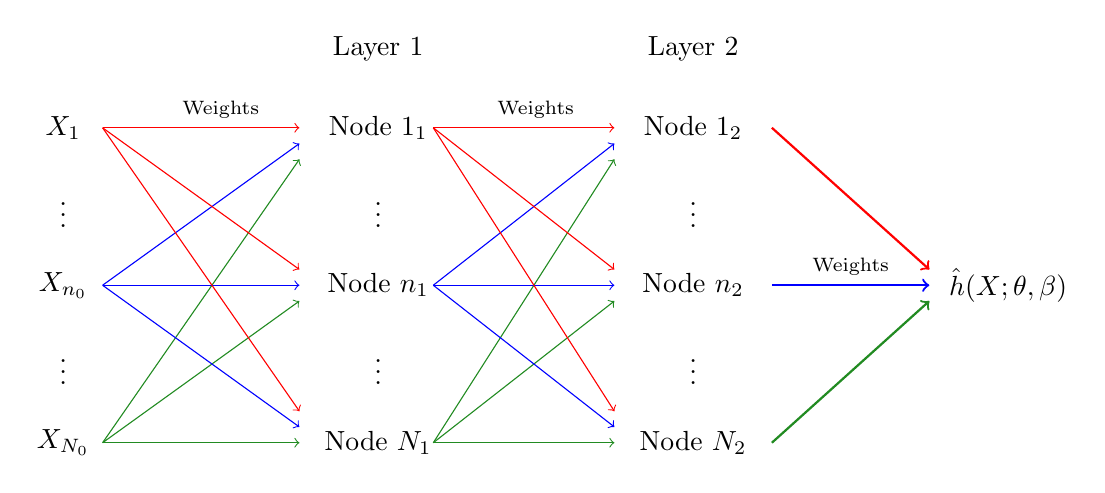
\begin{tikzpicture}[scale=1]
			\node at (0,8) {$X_1$};
			\node at (-0,7) {$\vdots$};
			\node at (0,6) {$X_{n_0}$};
			\node at (-0,5) {$\vdots$};
			\node at (0,4) {$X_{N_0}$};
			
			\node at (4,9) {Layer 1};
			\node at (4,8) {Node $1_1$};
			\node at (4,7) {$\vdots$};
			\node at (4,6) {Node $n_1$};
			\node at (4,5) {$\vdots$};
			\node at (4,4) {Node $N_1$};
			
			\node at (8,9) {Layer 2};
			\node at (8,8) {Node $1_2$};
			\node at (8,7) {$\vdots$};
			\node at (8,6) {Node $n_2$};
			\node at (8,5) {$\vdots$};
			\node at (8,4) {Node $N_2$};
			
			\node at (12,6) {$\hat{h}(X;\theta,\beta)$};
			
			\node[above] at (2,8) {\scriptsize Weights};
			\node[above] at (6,8) {\scriptsize Weights};
			\node[above] at (10,6) {\scriptsize Weights};
			
			\draw[->,red] (0.5,8)--(3,8);
			\draw[->,blue] (0.5,6)--(3,7.8);
			\draw[->,ForestGreen] (0.5,4)--(3,7.6);
			
			\draw[->,red] (0.5,8)--(3,6.2);
			\draw[->,blue] (0.5,6)--(3,6);
			\draw[->,ForestGreen] (0.5,4)--(3,5.8);
			
			
			\draw[->,red] (0.5,8)--(3,4.4);
			\draw[->,blue] (0.5,6)--(3,4.2);
			\draw[->,ForestGreen] (0.5,4)--(3,4);
			
			\draw[->,red] (4.7,8)--(7,8);
			\draw[->,blue] (4.7,6)--(7,7.8);
			\draw[->,ForestGreen] (4.7,4)--(7,7.6);
			
			\draw[->,red] (4.7,8)--(7,6.2);
			\draw[->,blue] (4.7,6)--(7,6);
			\draw[->,ForestGreen] (4.7,4)--(7,5.8);
			
			
			\draw[->,red] (4.7,8)--(7,4.4);
			\draw[->,blue] (4.7,6)--(7,4.2);
			\draw[->,ForestGreen] (4.7,4)--(7,4);
			
			\draw[->,red,thick] (9,8)--(11,6.2);
			\draw[->,blue,thick] (9,6)--(11,6);
			\draw[->,ForestGreen,thick] (9,4)--(11,5.8);
		\end{tikzpicture}
		\caption{A Two-Layer Neural Network}
		\label{fig:neural_net}
	\end{figure}
\end{algorithm}

\begin{remark}
	Ryan has a really lovely example of this in the Real Business Cycle model, you can work through the code yourself.
\end{remark}

\begin{remark}
	Andrew Ng's \href{https://cs229.stanford.edu/lectures-spring2022/main_notes.pdf}{CS 229 Lecture Notes} have an excellent treatment of this in particular and machine learning in general. See Chapter 7.2.
\end{remark}

\end{document}